\chapter{SIBench Architecture Details}
what is the purpose of providing the default ontology and data?
the full document of the ontology of derived LUBM ontology
how did you convert the lubm data into stream? 
what is the rule of assigning the expiration timestamp, and trust score?
how did you simulate the stream so that it has constant/various streaming rate? 

why cannot I create a strategy in run time?
I have updated the lubm ontology
I have converted the lubm streaming data
how did I allocate the expiration timestamp
how did I allocate the trustscore

The probability is taken from the real life observation on the traffic.
Normally there are two rush periods in a day, one in morning and one in afternoon, each of the rush hour lasts approximately 2 hours. 
So the peak probability of 4/24 = 1/6. 
22:00 to 2:00 next day is quietest period where minimum traffic flow will be, so P{rate = 0} = 4/24 = 1/6. 
The rest of the probability is for an in-between rate. 

\chapter{SIGenBench Benchmark Results Visualization}
This chapter lists the results visualizations of all the experiments in Chapter 6. 
The visualizations provide a more intuitive and detailed view of each strategy's performance, which makes it easy to analyze the advantages and disadvantages for each strategy in different scenarios. 
%%%%%%%%%%%%%%%%%%%%%%%%%
%%%%%%%%%%%%%%%%%%%%%%%%%
%%   query relevance %%%%
%%%%%%%%%%%%%%%%%%%%%%%%%
%%%%%%%%%%%%%%%%%%%%%%%%%
\begin{figure}[!htbp]
    \centering
    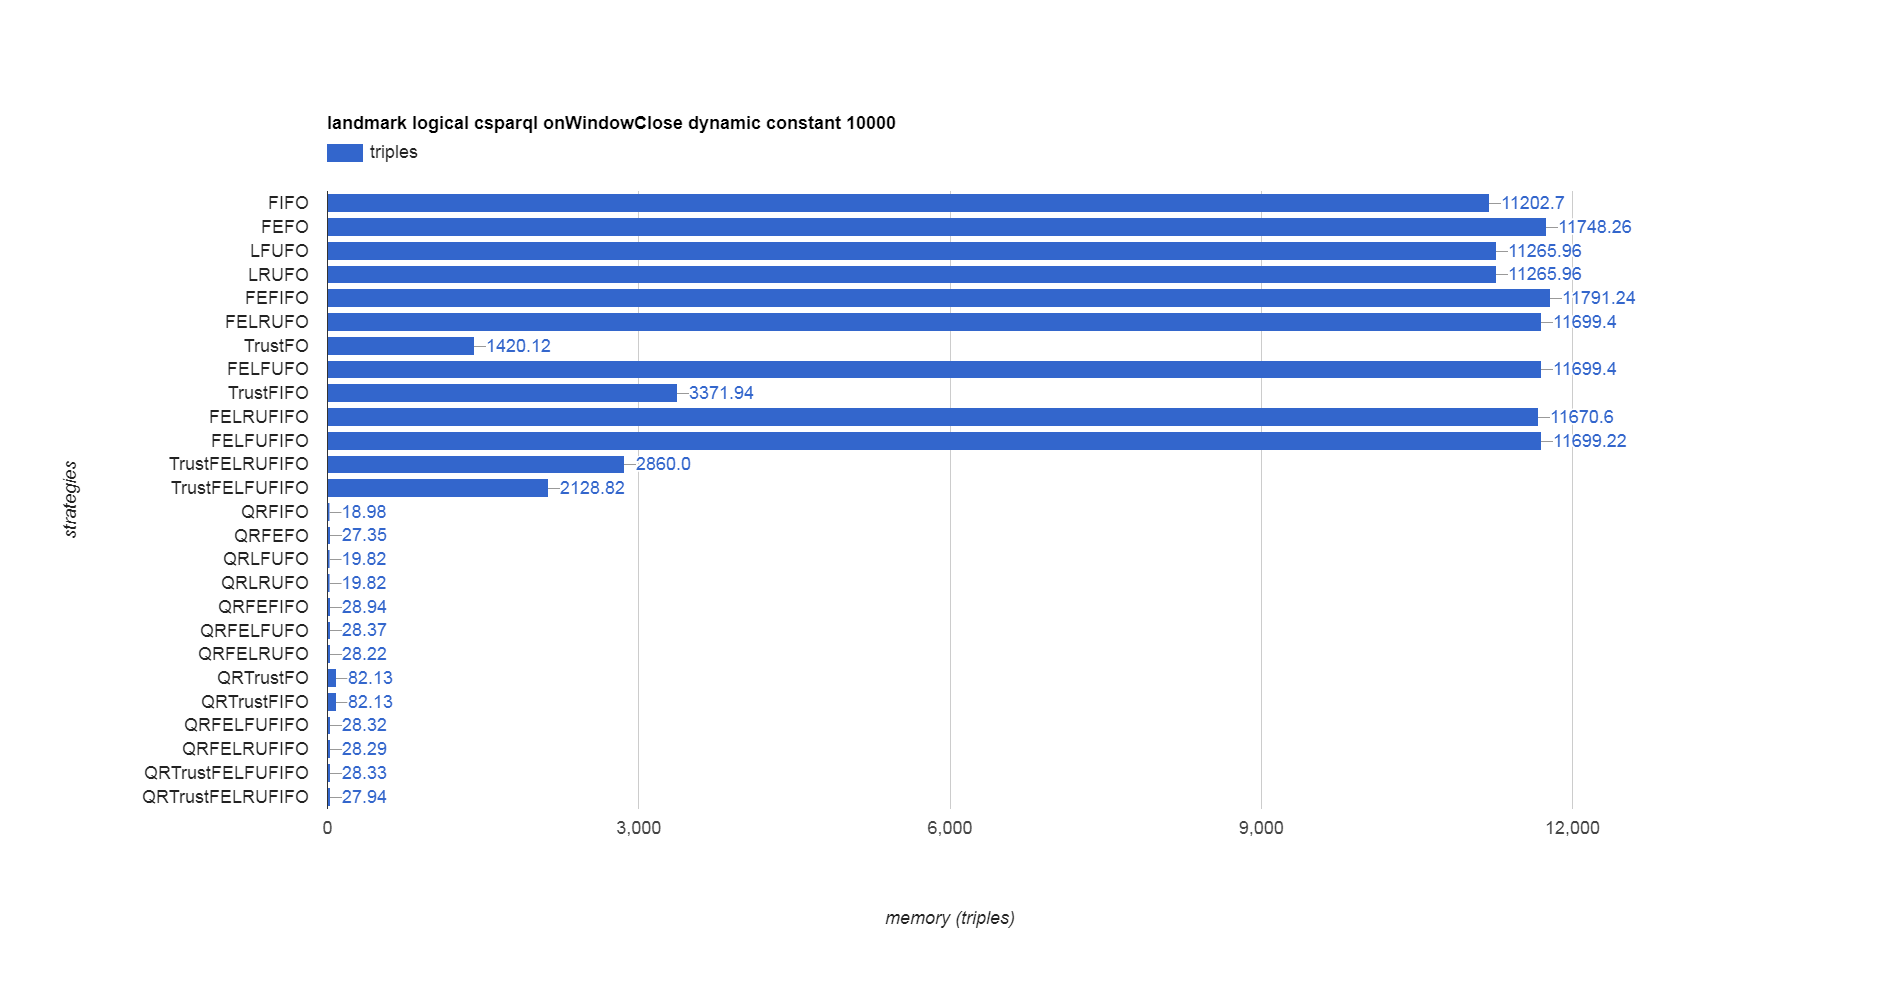
\includegraphics[width=\textwidth]{img/app3-gqr-m.png}
    \caption{Good Query Relevance Filter Query Memory Consumption}
\end{figure}
\begin{figure}[!htbp]
    \centering
    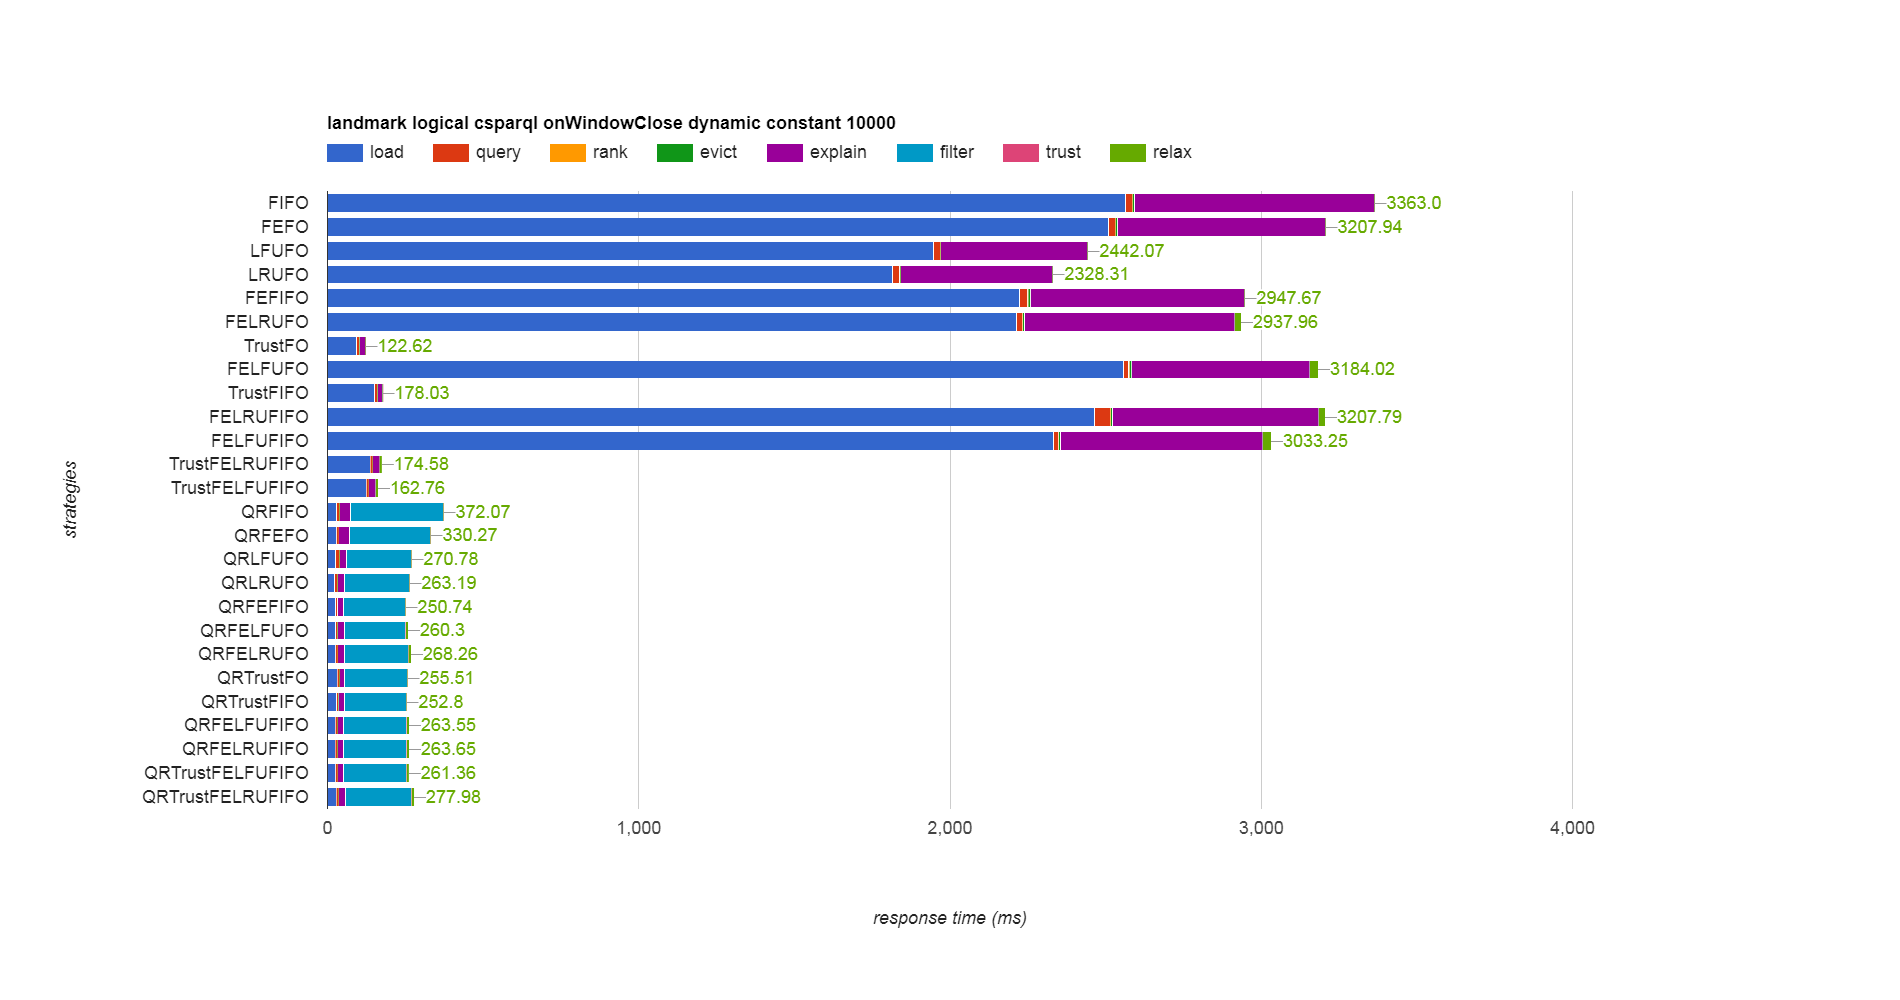
\includegraphics[width=\textwidth]{img/app3-gqr-r.png}
    \caption{Good Query Relevance Filter Query Response Time}
\end{figure}
\begin{figure}[!htbp]
    \centering
    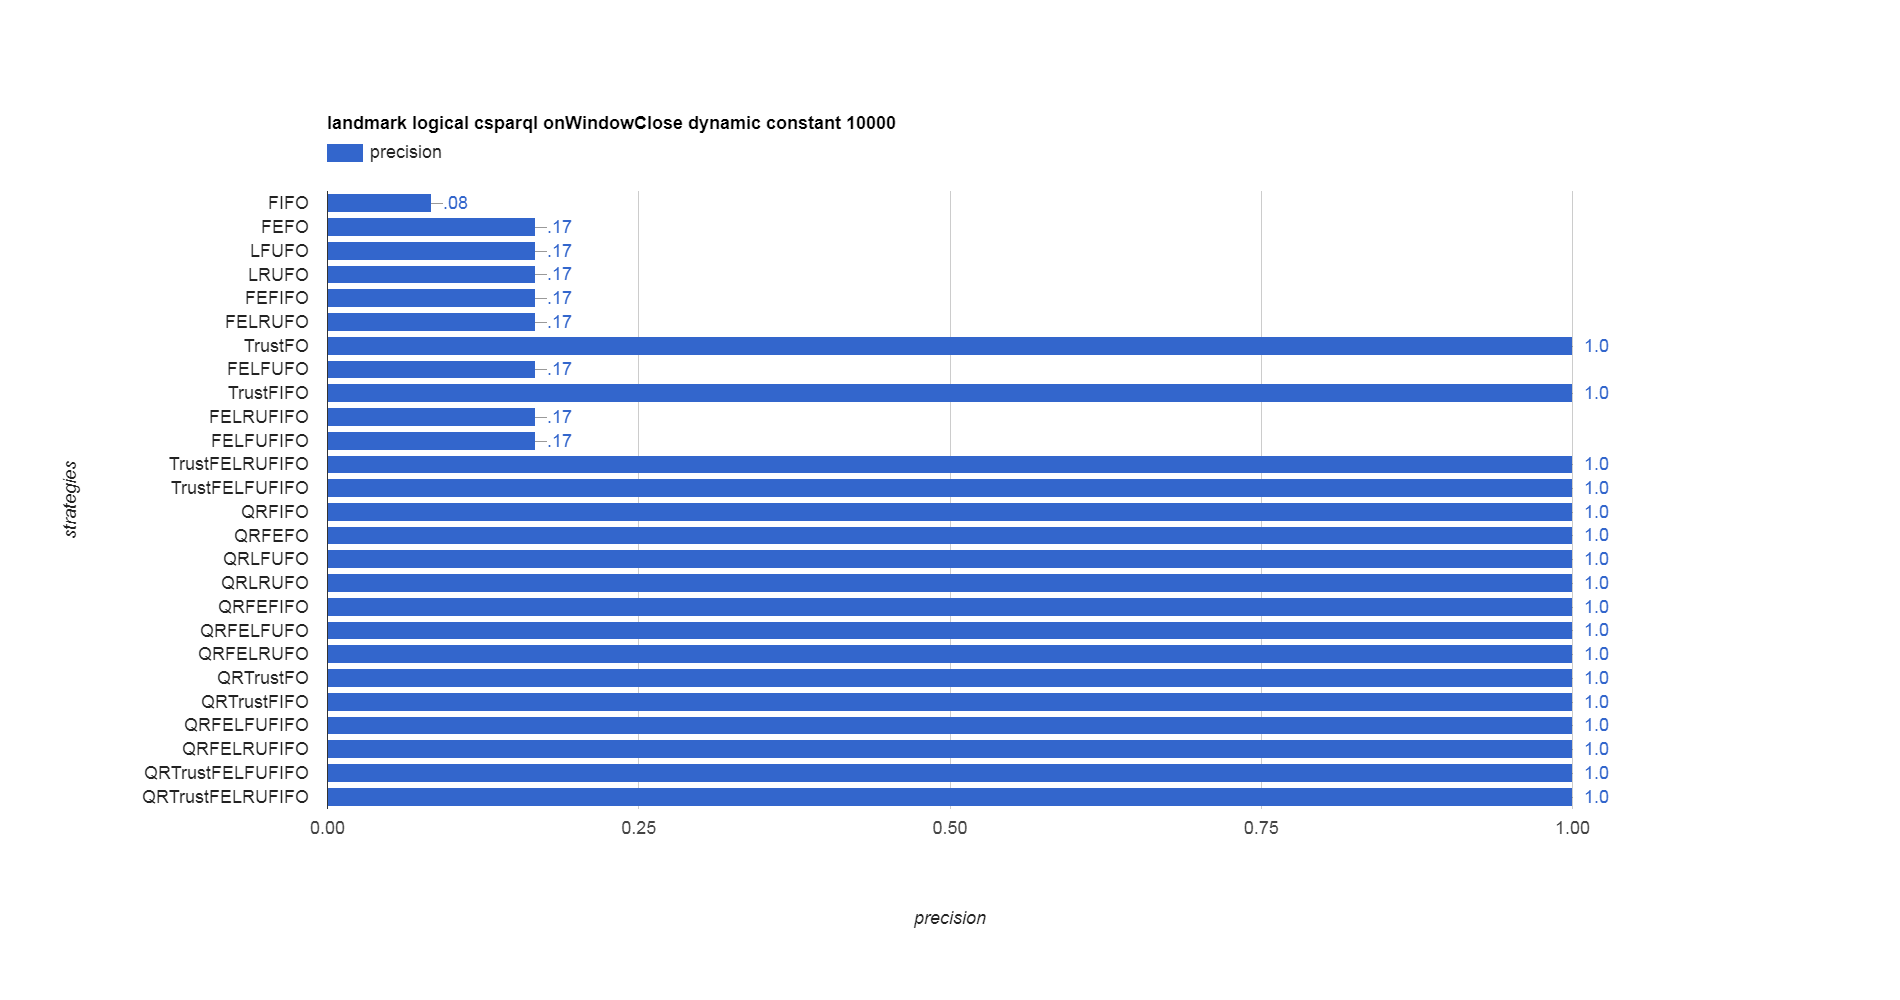
\includegraphics[width=\textwidth]{img/app3-gqr-p.png}
    \caption{Good Query Relevance Filter Query Precision}
\end{figure}
\begin{figure}[!htbp]
    \centering
    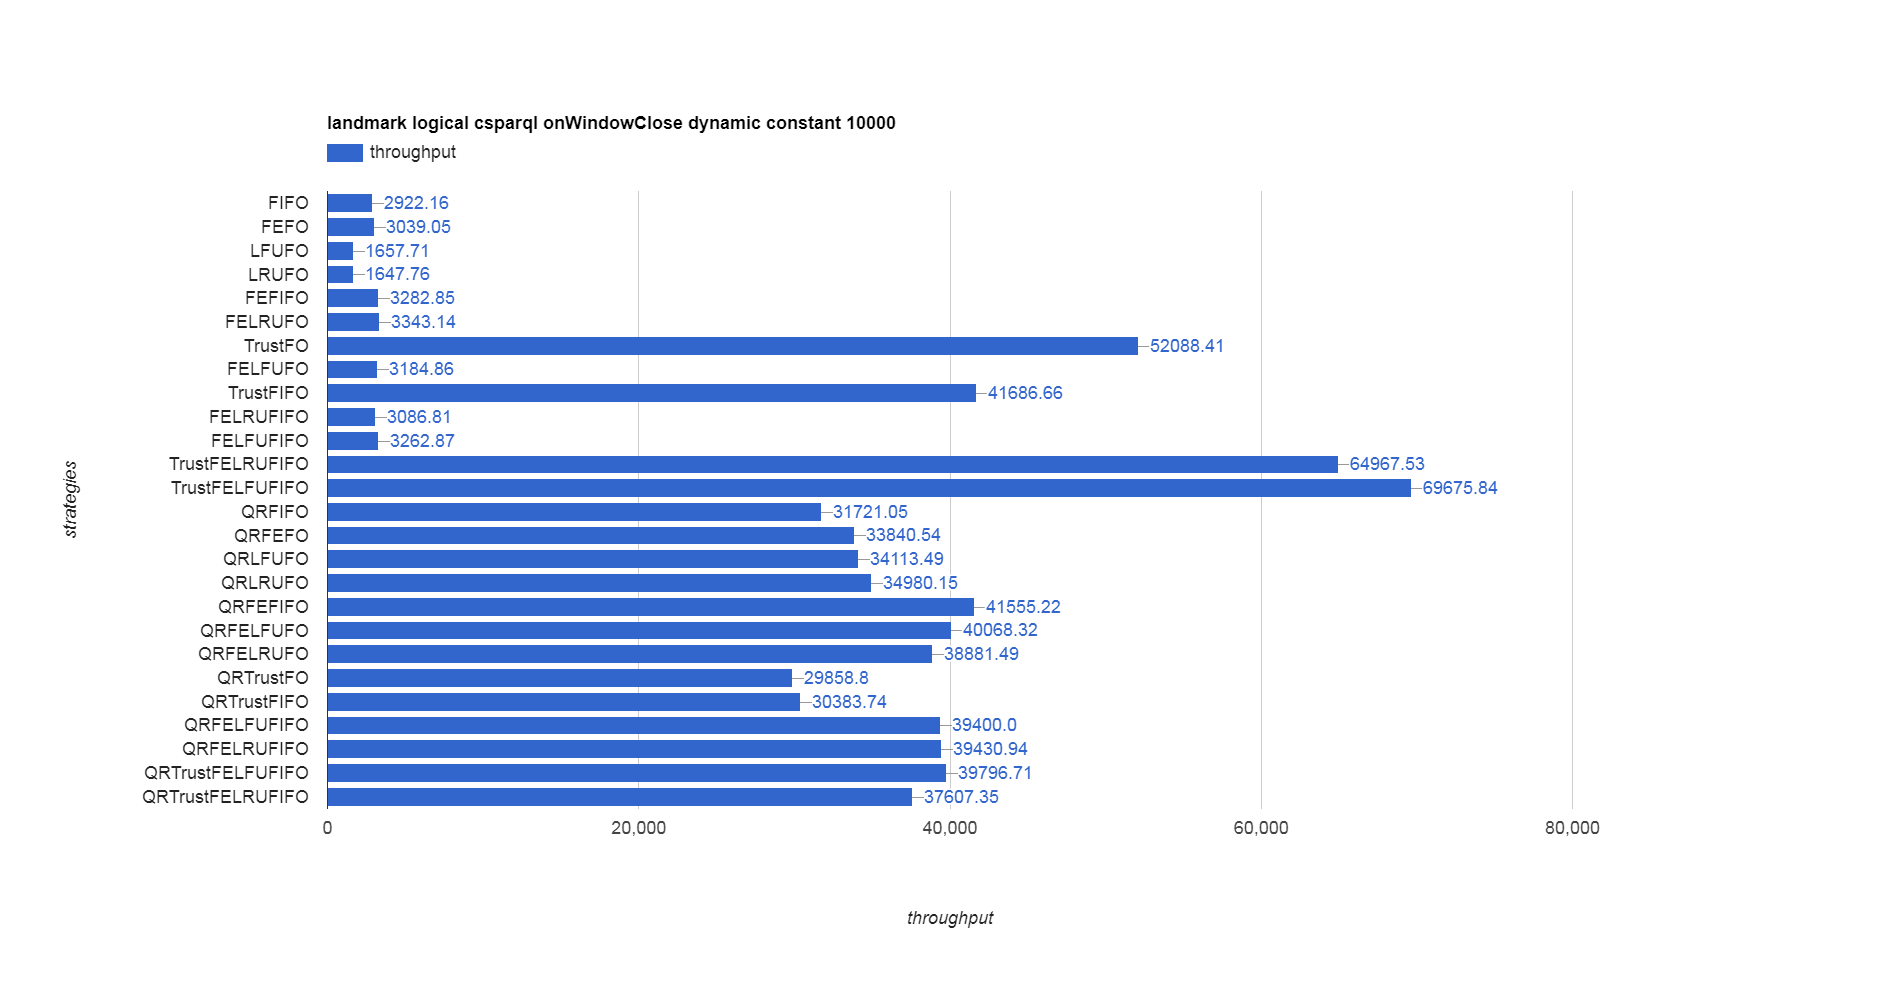
\includegraphics[width=\textwidth]{img/app3-gqr-t.png}
    \caption{Good Query Relevance Filter Query Throughput}
\end{figure}
\begin{figure}[!htbp]
    \centering
    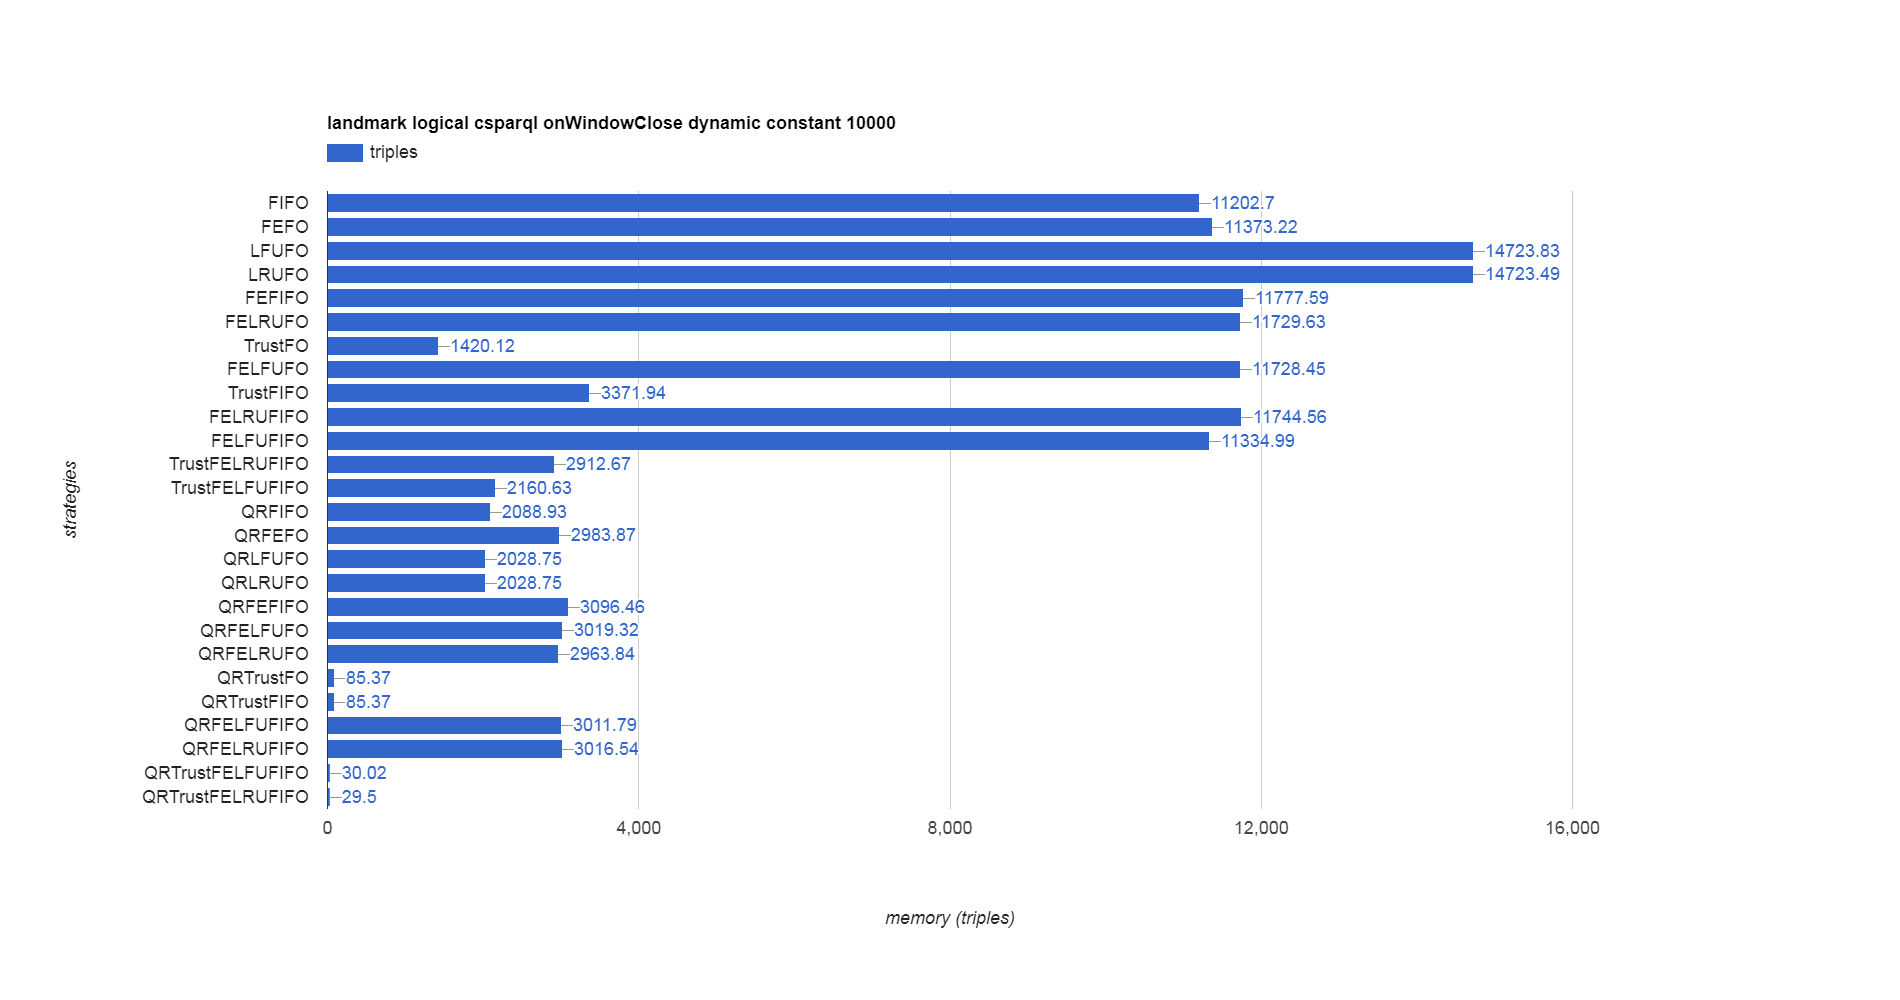
\includegraphics[width=\textwidth]{img/app3-oqr-m.png}
    \caption{OK Query Relevance Filter Query Memory Consumption}
\end{figure}
\begin{figure}[!htbp]
    \centering
    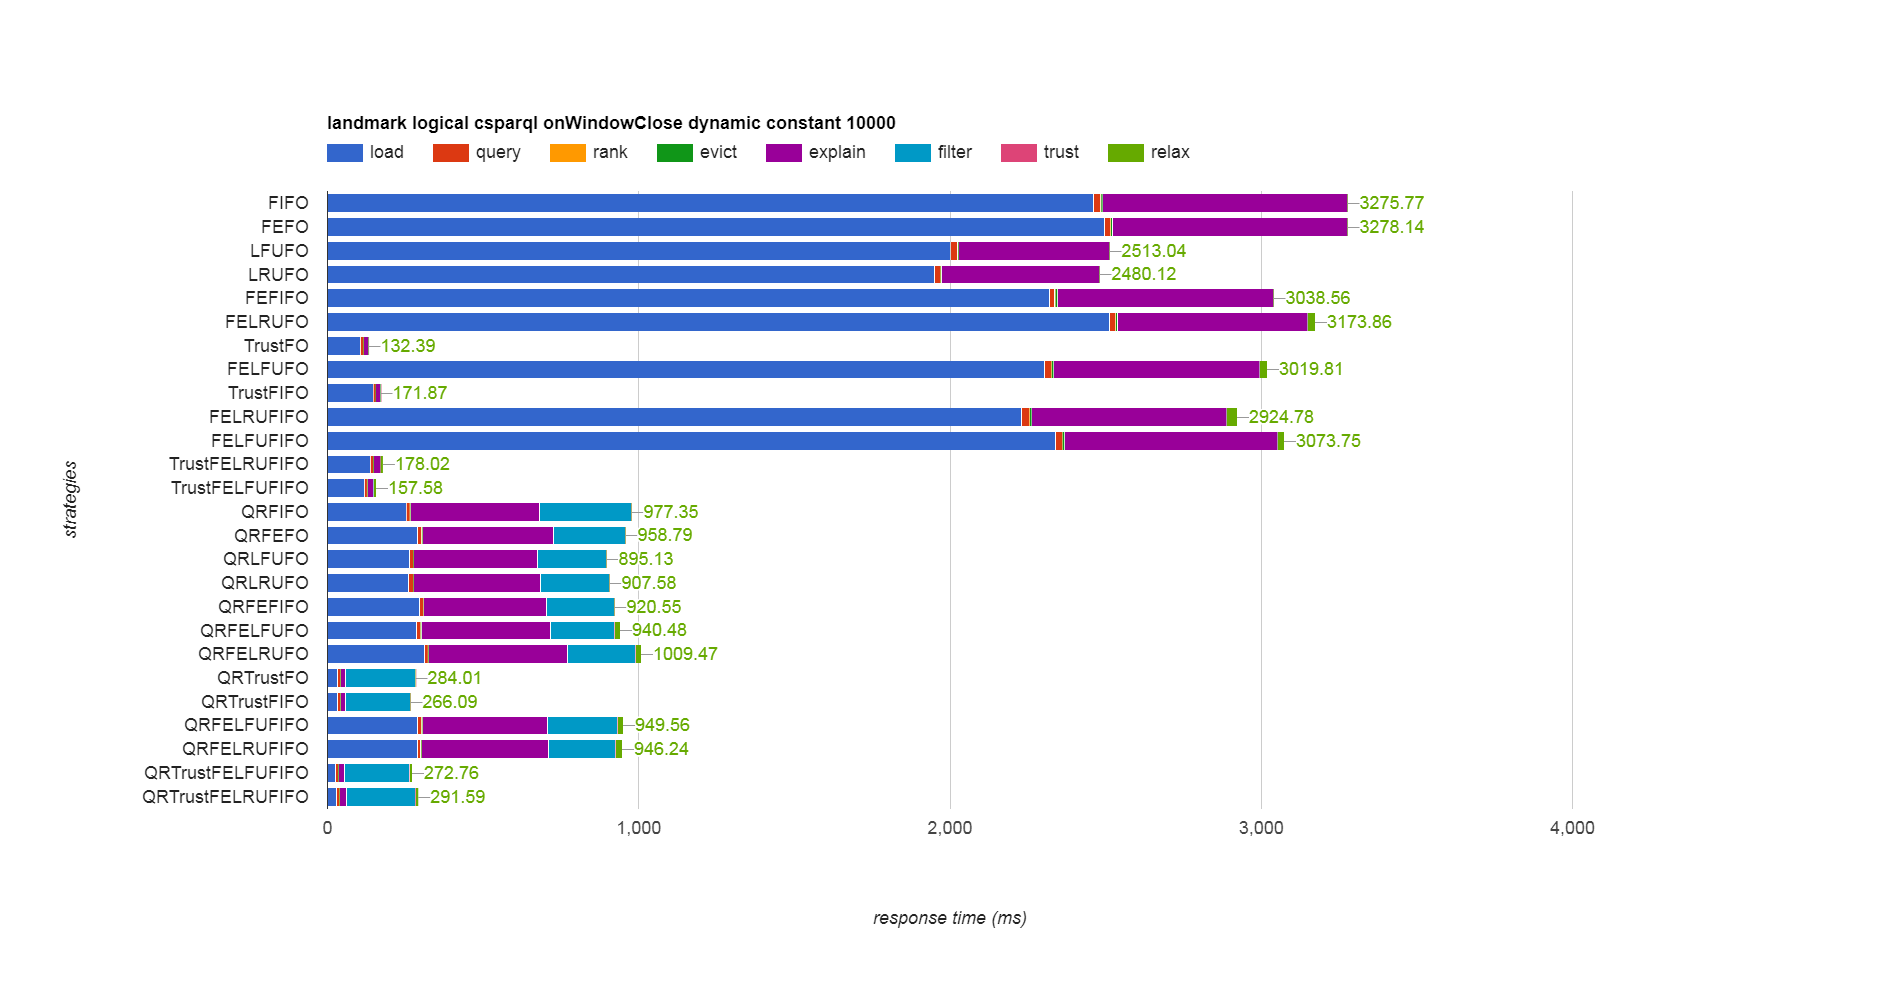
\includegraphics[width=\textwidth]{img/app3-oqr-r.png}
    \caption{OK Query Relevance Filter Query Response Time}
\end{figure}
\begin{figure}[!htbp]
    \centering
    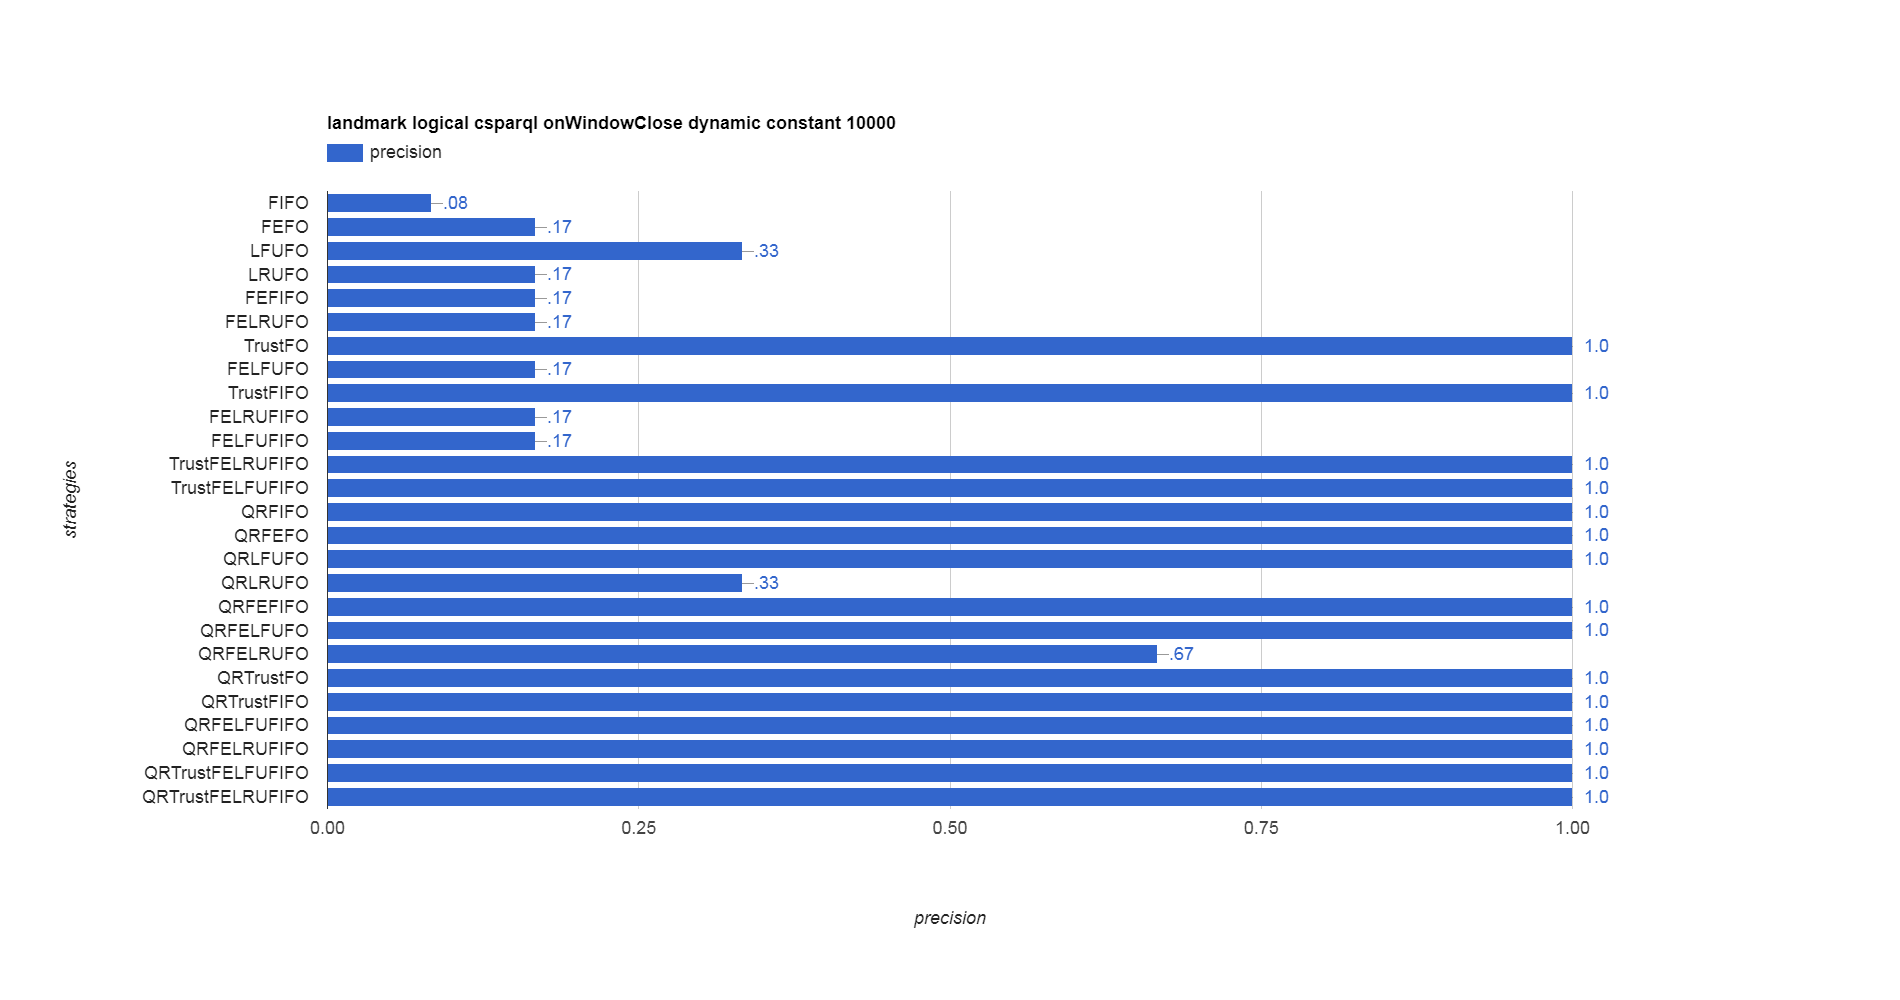
\includegraphics[width=\textwidth]{img/app3-oqr-p.png}
    \caption{OK Query Relevance Filter Query Precision}
\end{figure}
\begin{figure}[!htbp]
    \centering
    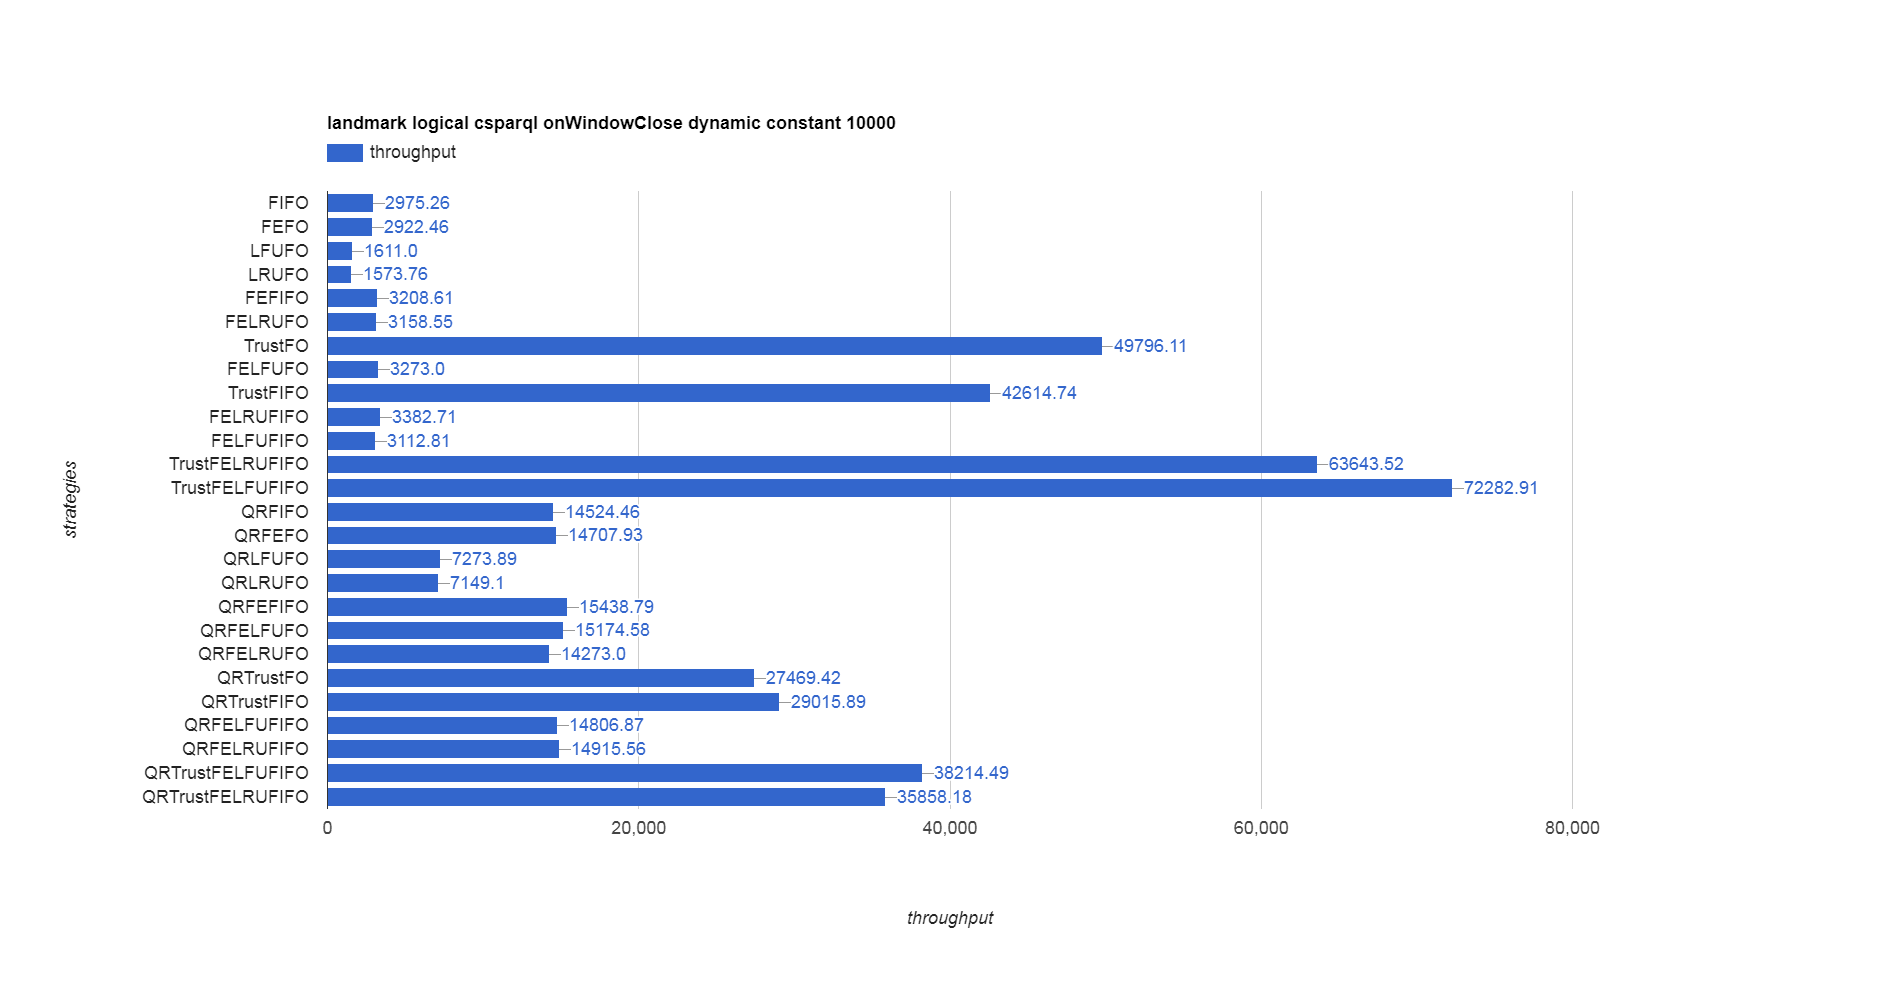
\includegraphics[width=\textwidth]{img/app3-oqr-t.png}
    \caption{OK Query Relevance Filter Query Throughput}
\end{figure}
\begin{figure}[!htbp]
    \centering
    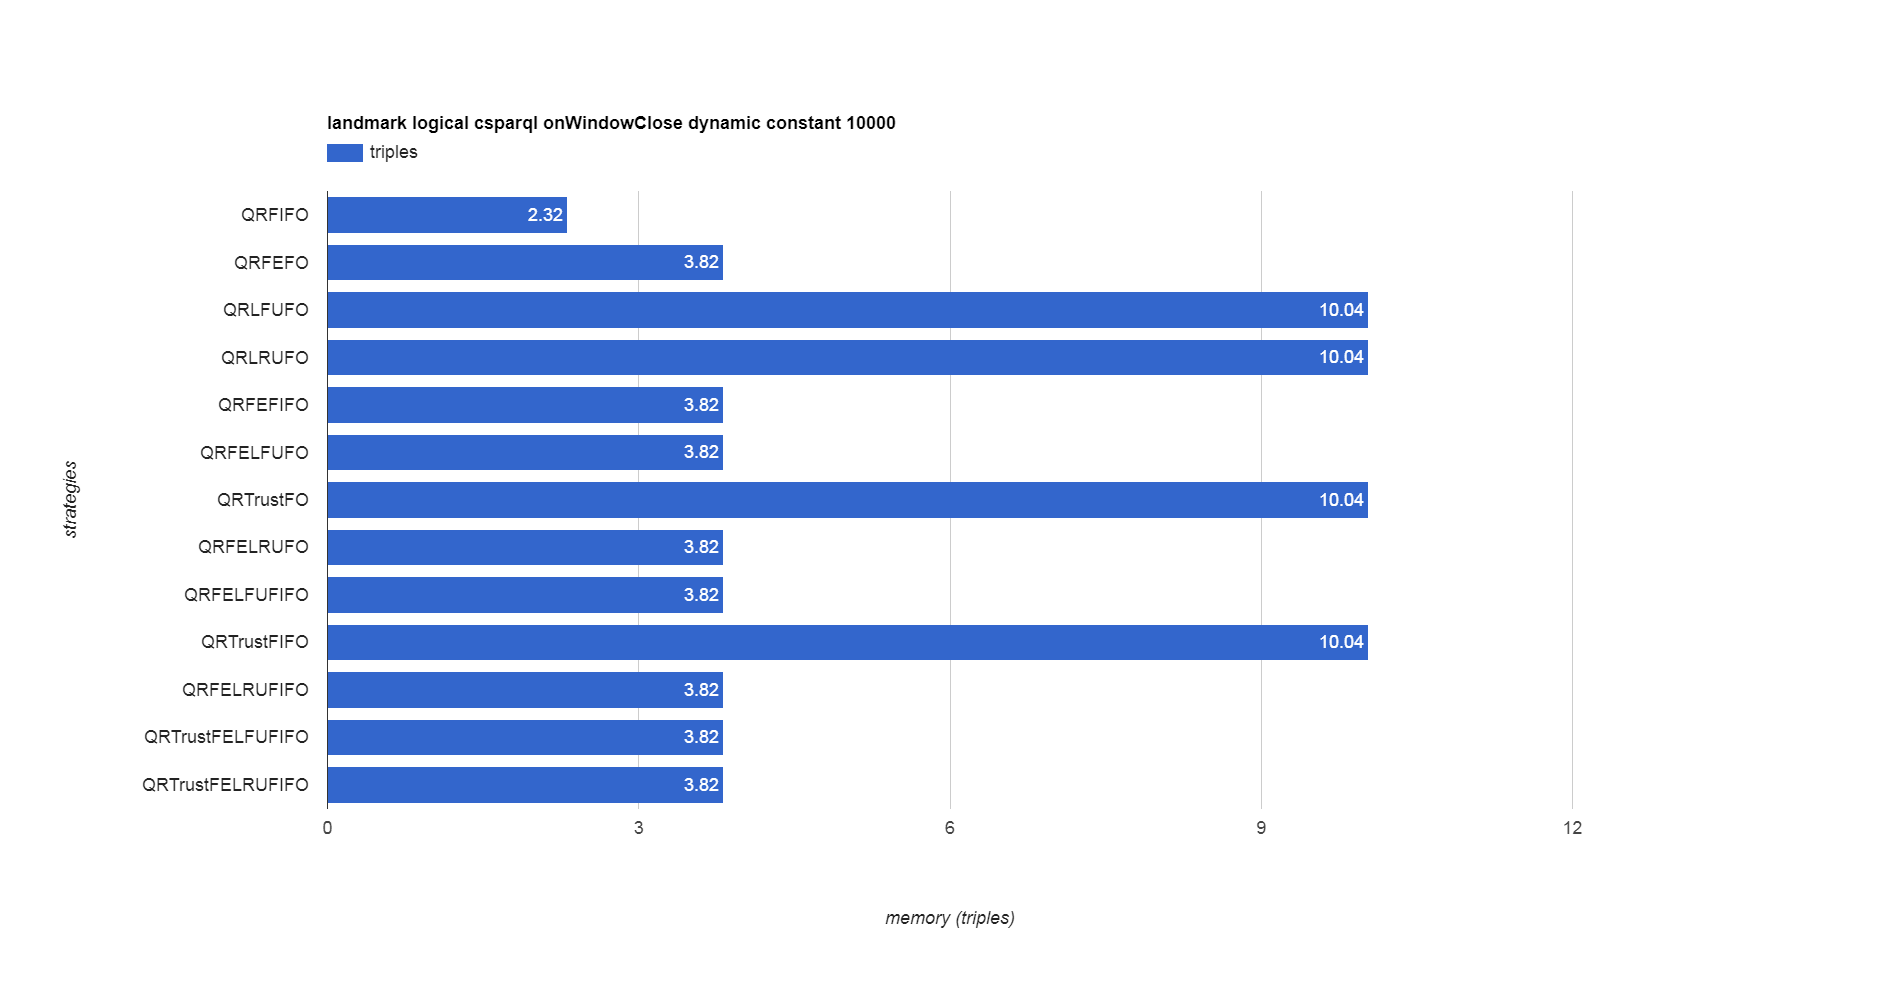
\includegraphics[width=\textwidth]{img/app3-bqr-m.png}
    \caption{Bad Query Relevance Filter Query Memory Consumption}
\end{figure}
\begin{figure}[!htbp]
    \centering
    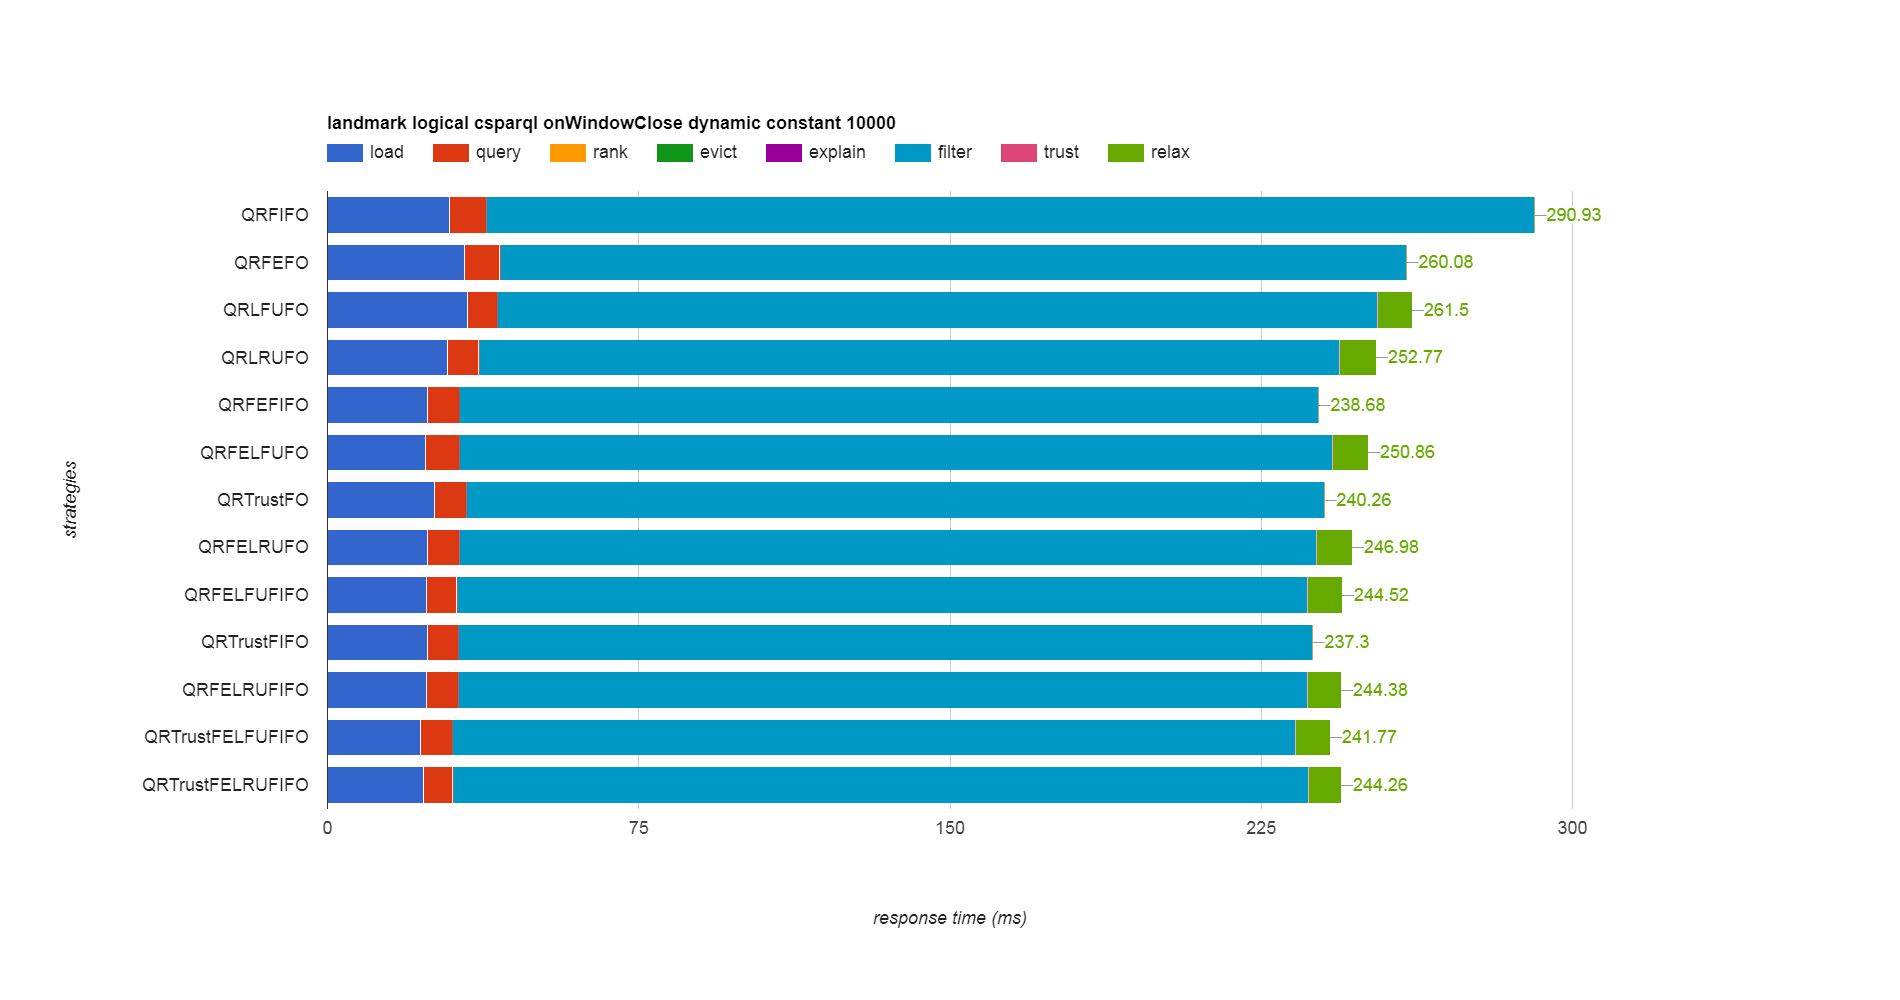
\includegraphics[width=\textwidth]{img/app3-bqr-r.png}
    \caption{Bad Query Relevance Filter Query Response Time}
\end{figure}
\begin{figure}[!htbp]
    \centering
    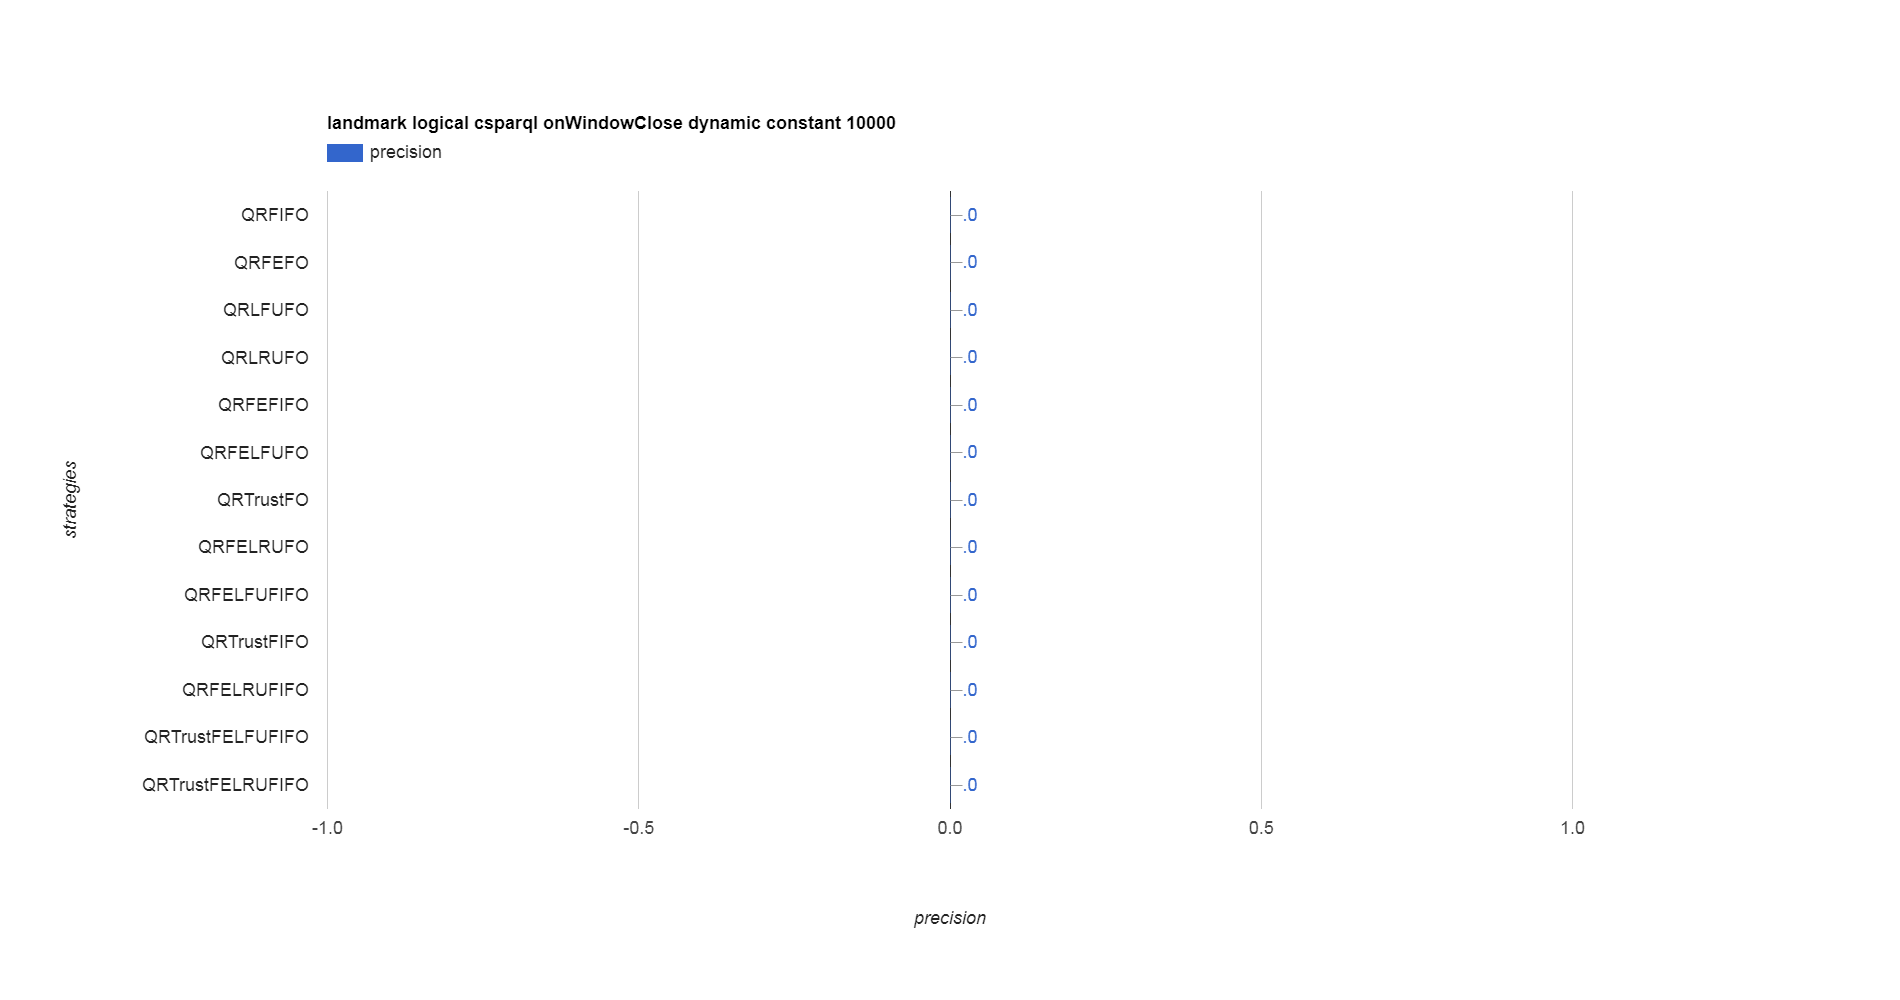
\includegraphics[width=\textwidth]{img/app3-bqr-p.png}
    \caption{Bad Query Relevance Filter Query Precision}
\end{figure}
\begin{figure}[!htbp]
    \centering
    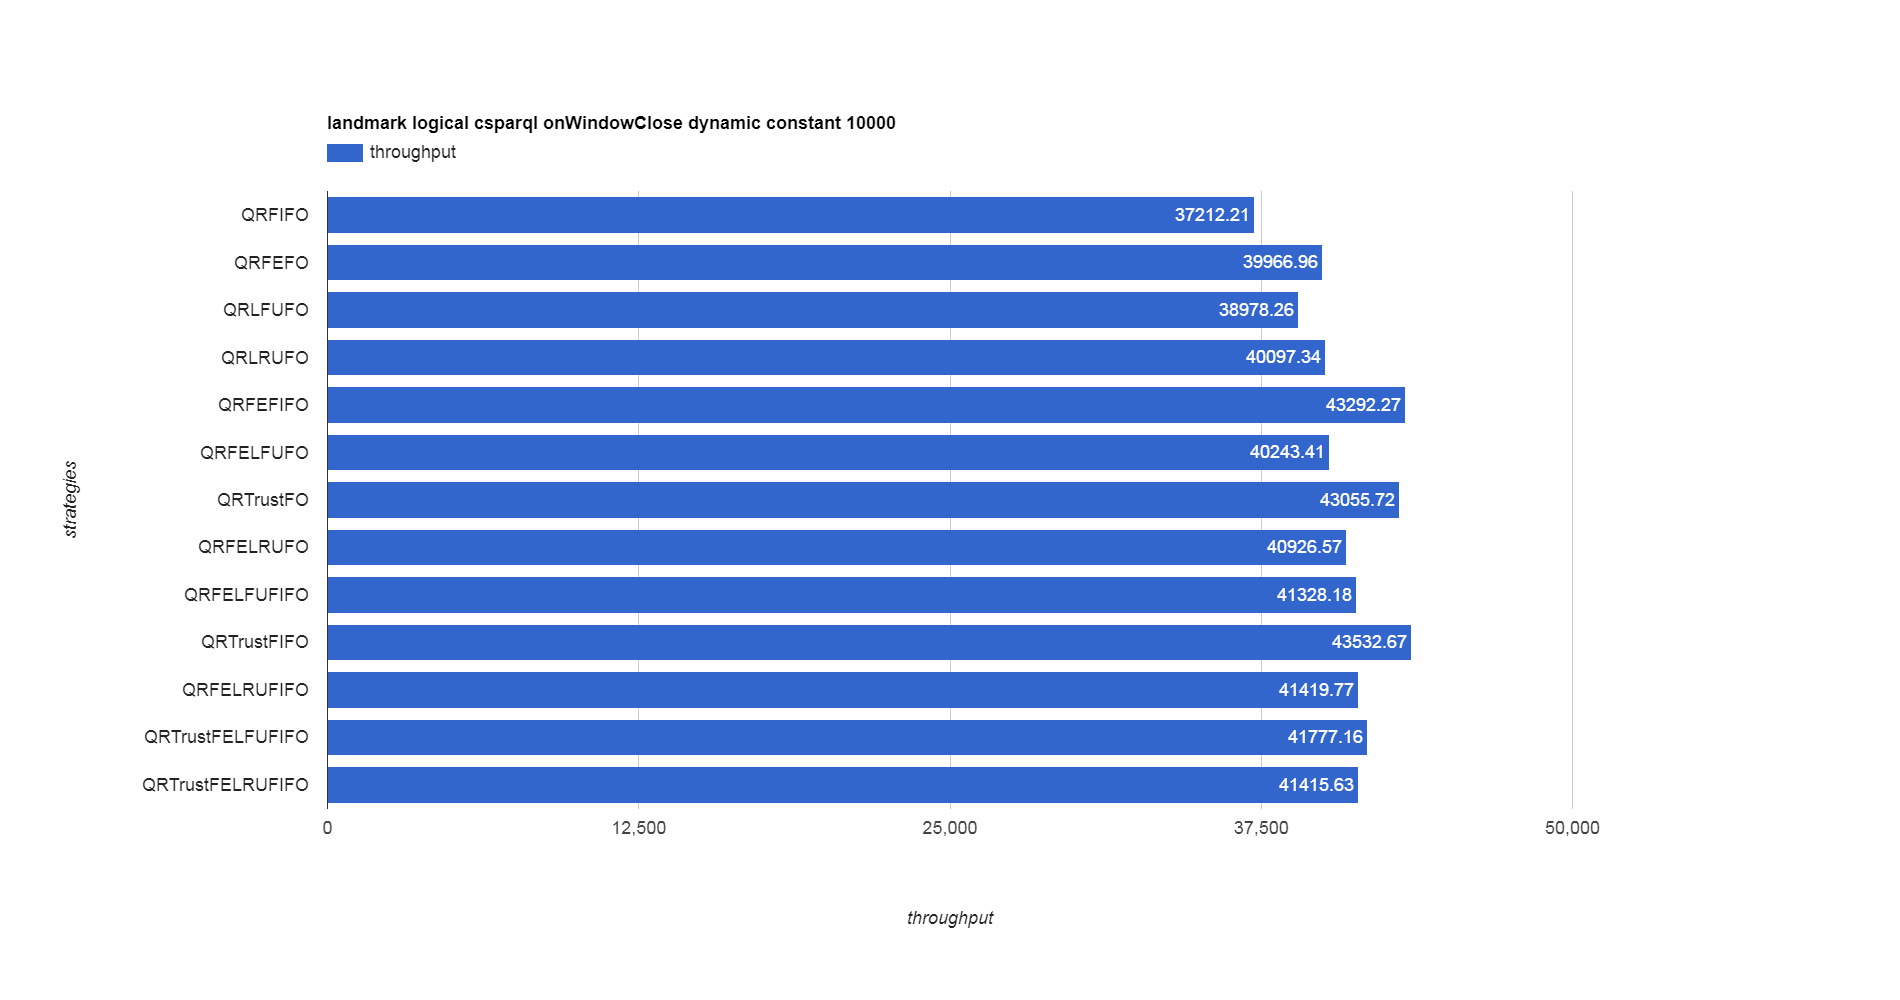
\includegraphics[width=\textwidth]{img/app3-bqr-t.png}
    \caption{Bad Query Relevance Filter Query Throughput}
\end{figure}
%%%%%%%%%%%%%%%%%%%%%%%%%
%%%%%%%%%%%%%%%%%%%%%%%%%
%% temporal provenance %%
%%%%%%%%%%%%%%%%%%%%%%%%%
%%%%%%%%%%%%%%%%%%%%%%%%%
\begin{figure}[!htbp]
    \centering
    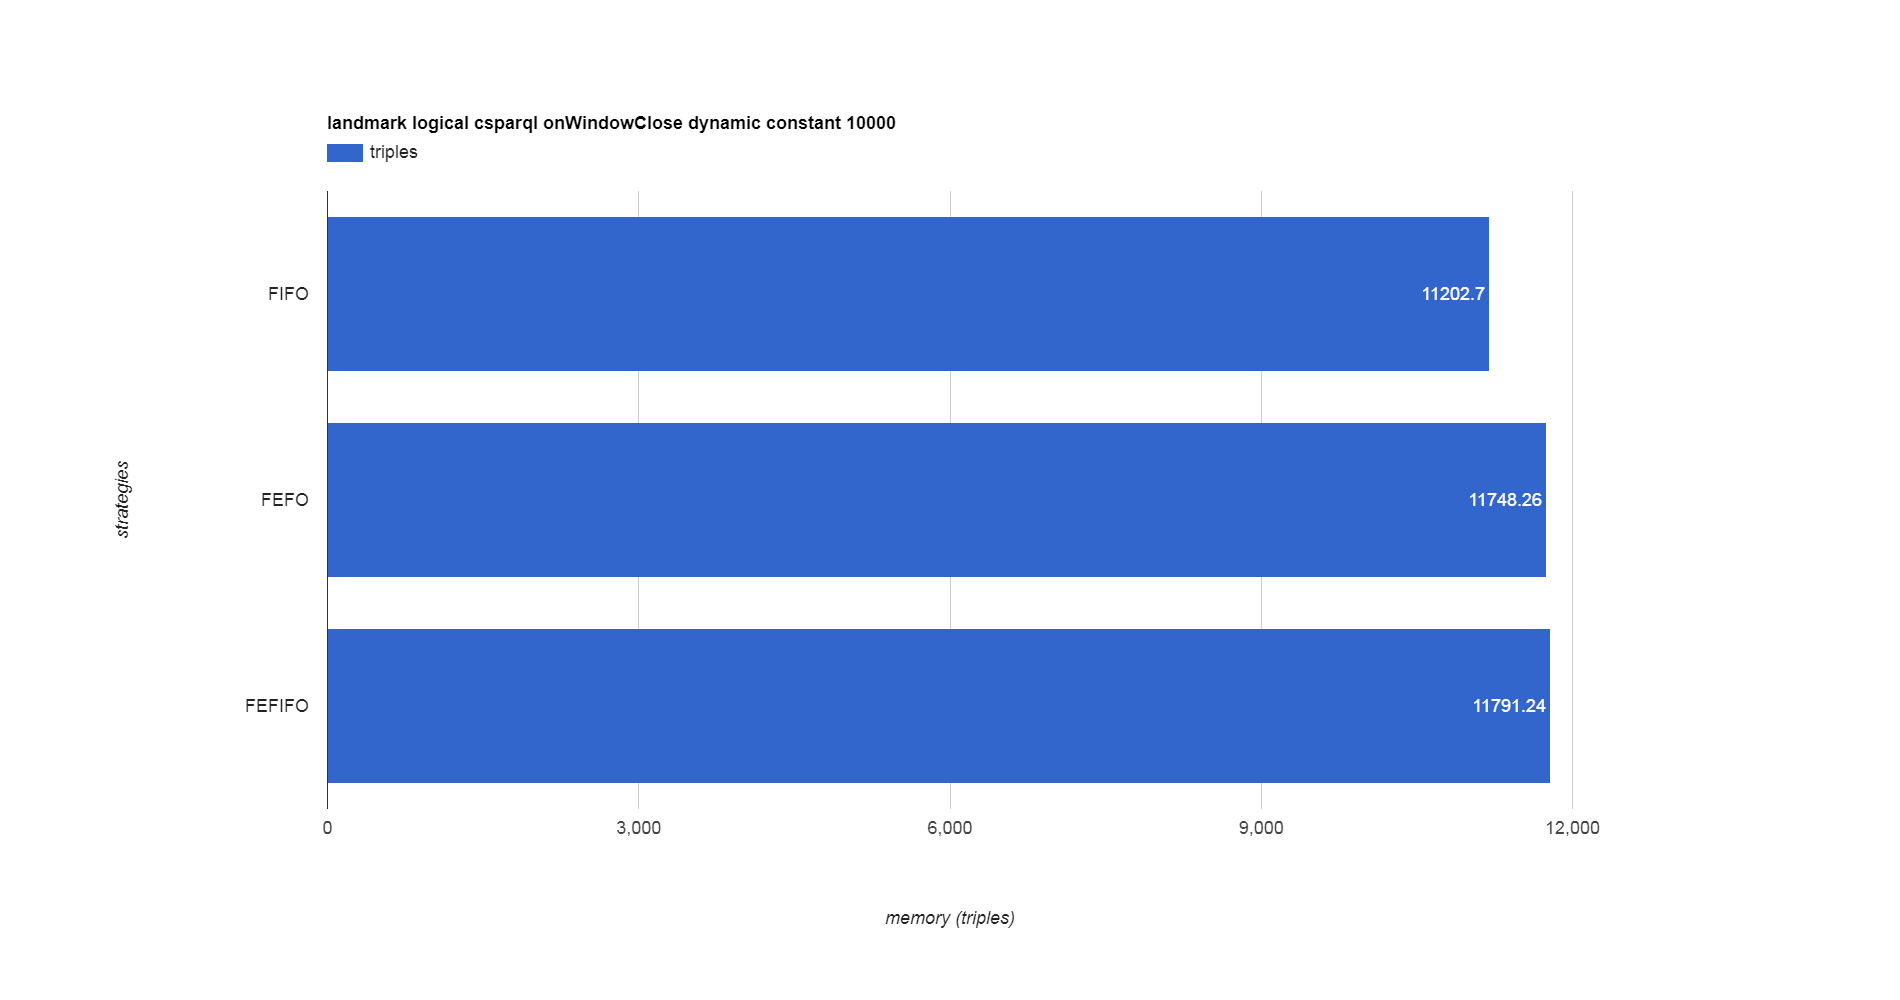
\includegraphics[width=\textwidth]{img/app3-ets-quick-m.png}
    \caption{Quick Data Expiration Memory Consumption}
\end{figure}
\begin{figure}[!htpb]
    \centering
    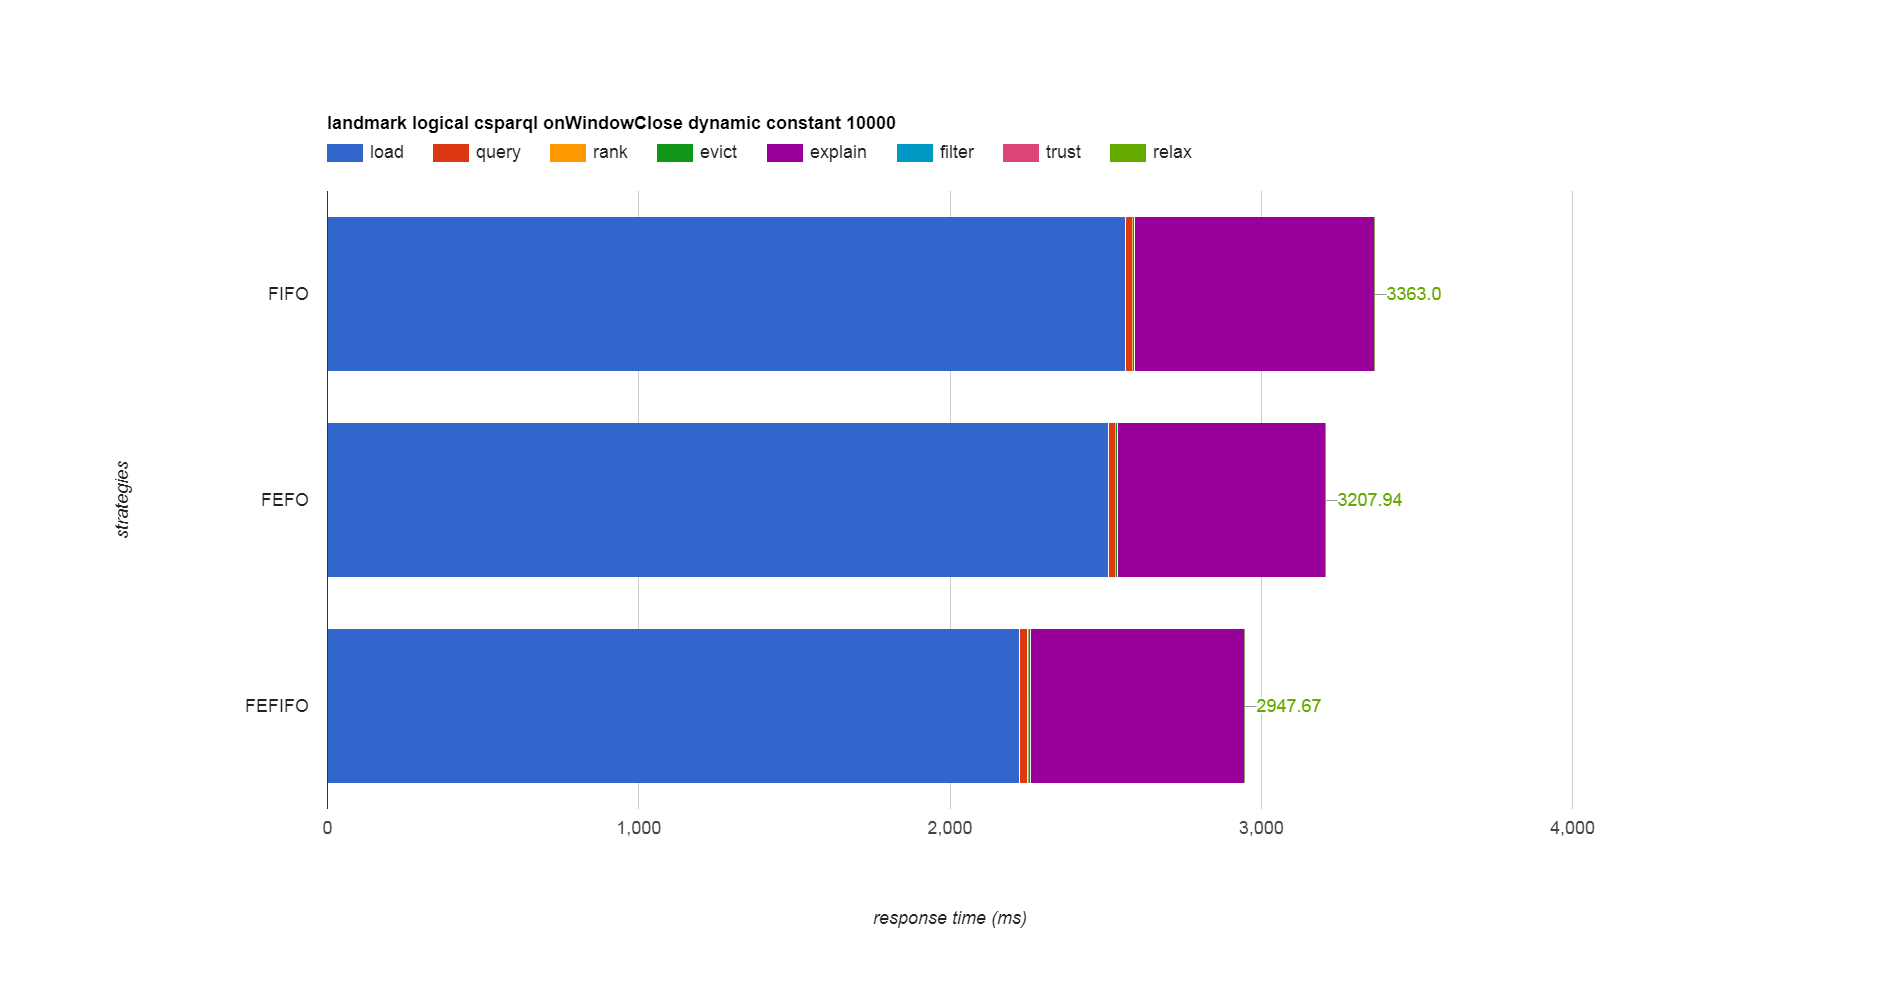
\includegraphics[width=\textwidth]{img/app3-ets-quick-r.png}
    \caption{Quick Data Expiration Response Time}
\end{figure}
\begin{figure}[!htbp]
    \centering
    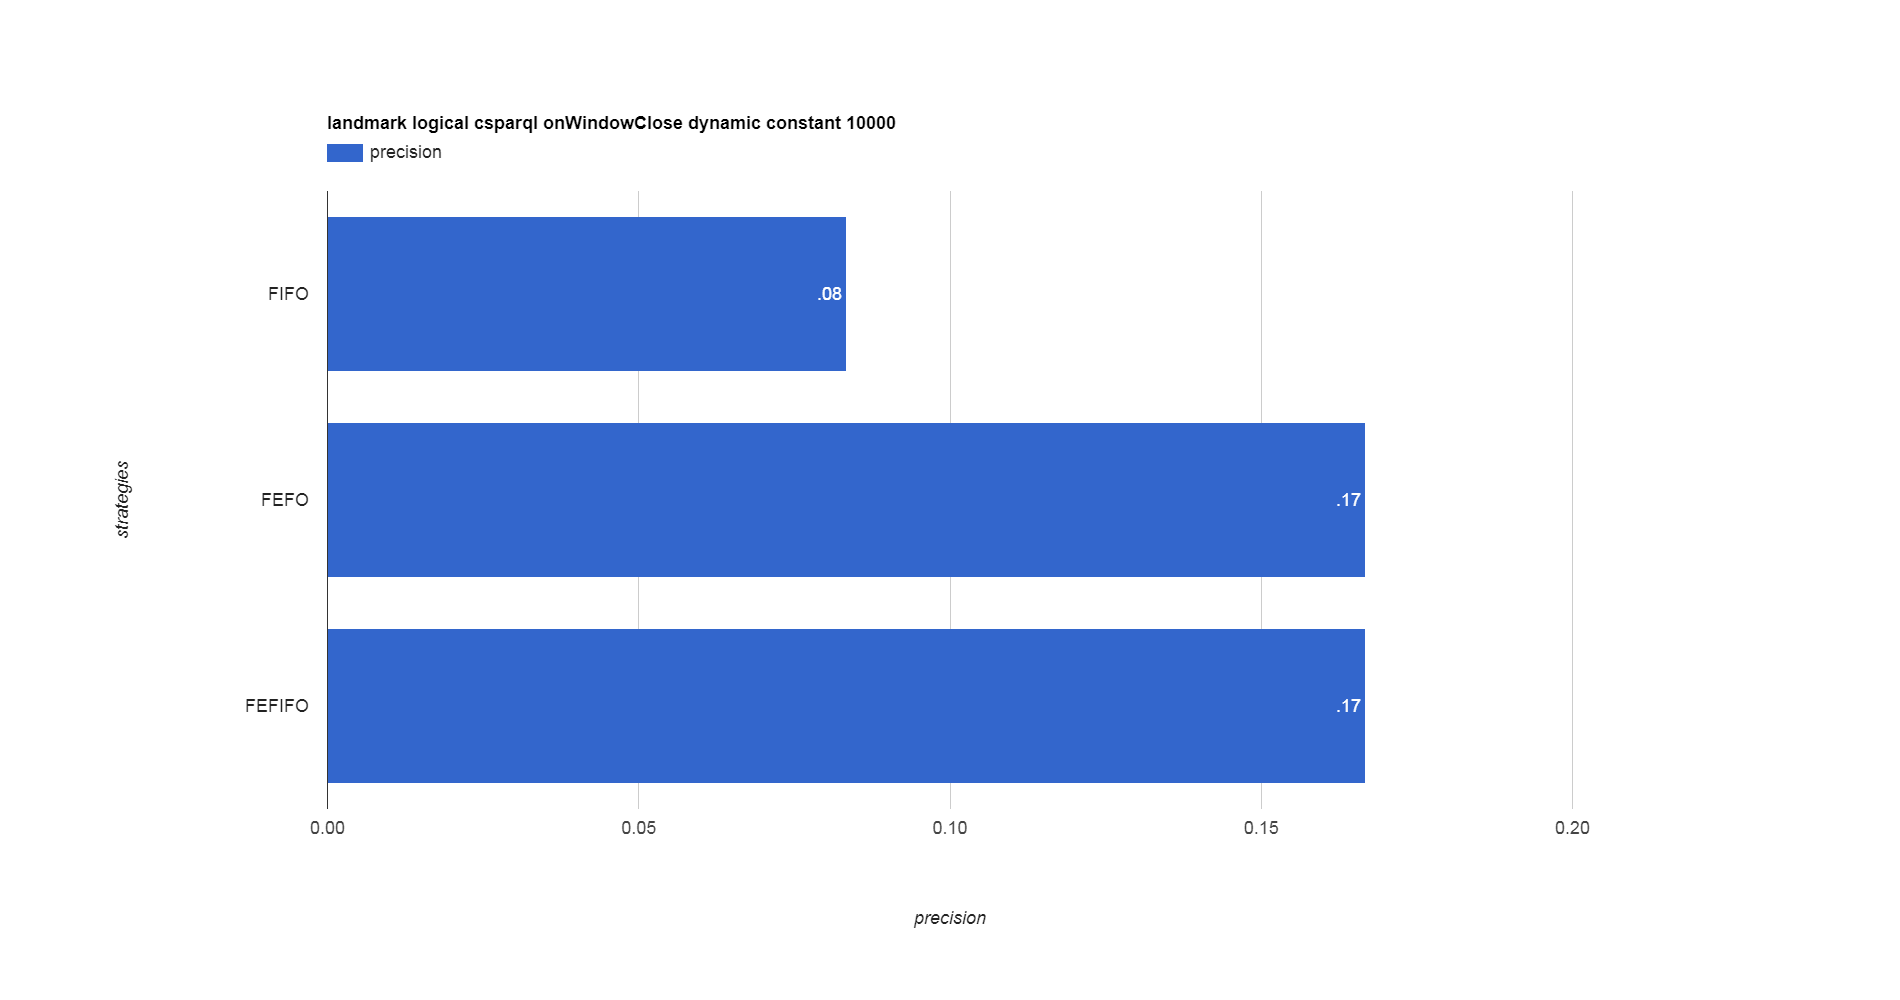
\includegraphics[width=\textwidth]{img/app3-ets-quick-p.png}
    \caption{Quick Data Expiration Precision}
\end{figure}
\begin{figure}[!htbp]
    \centering
    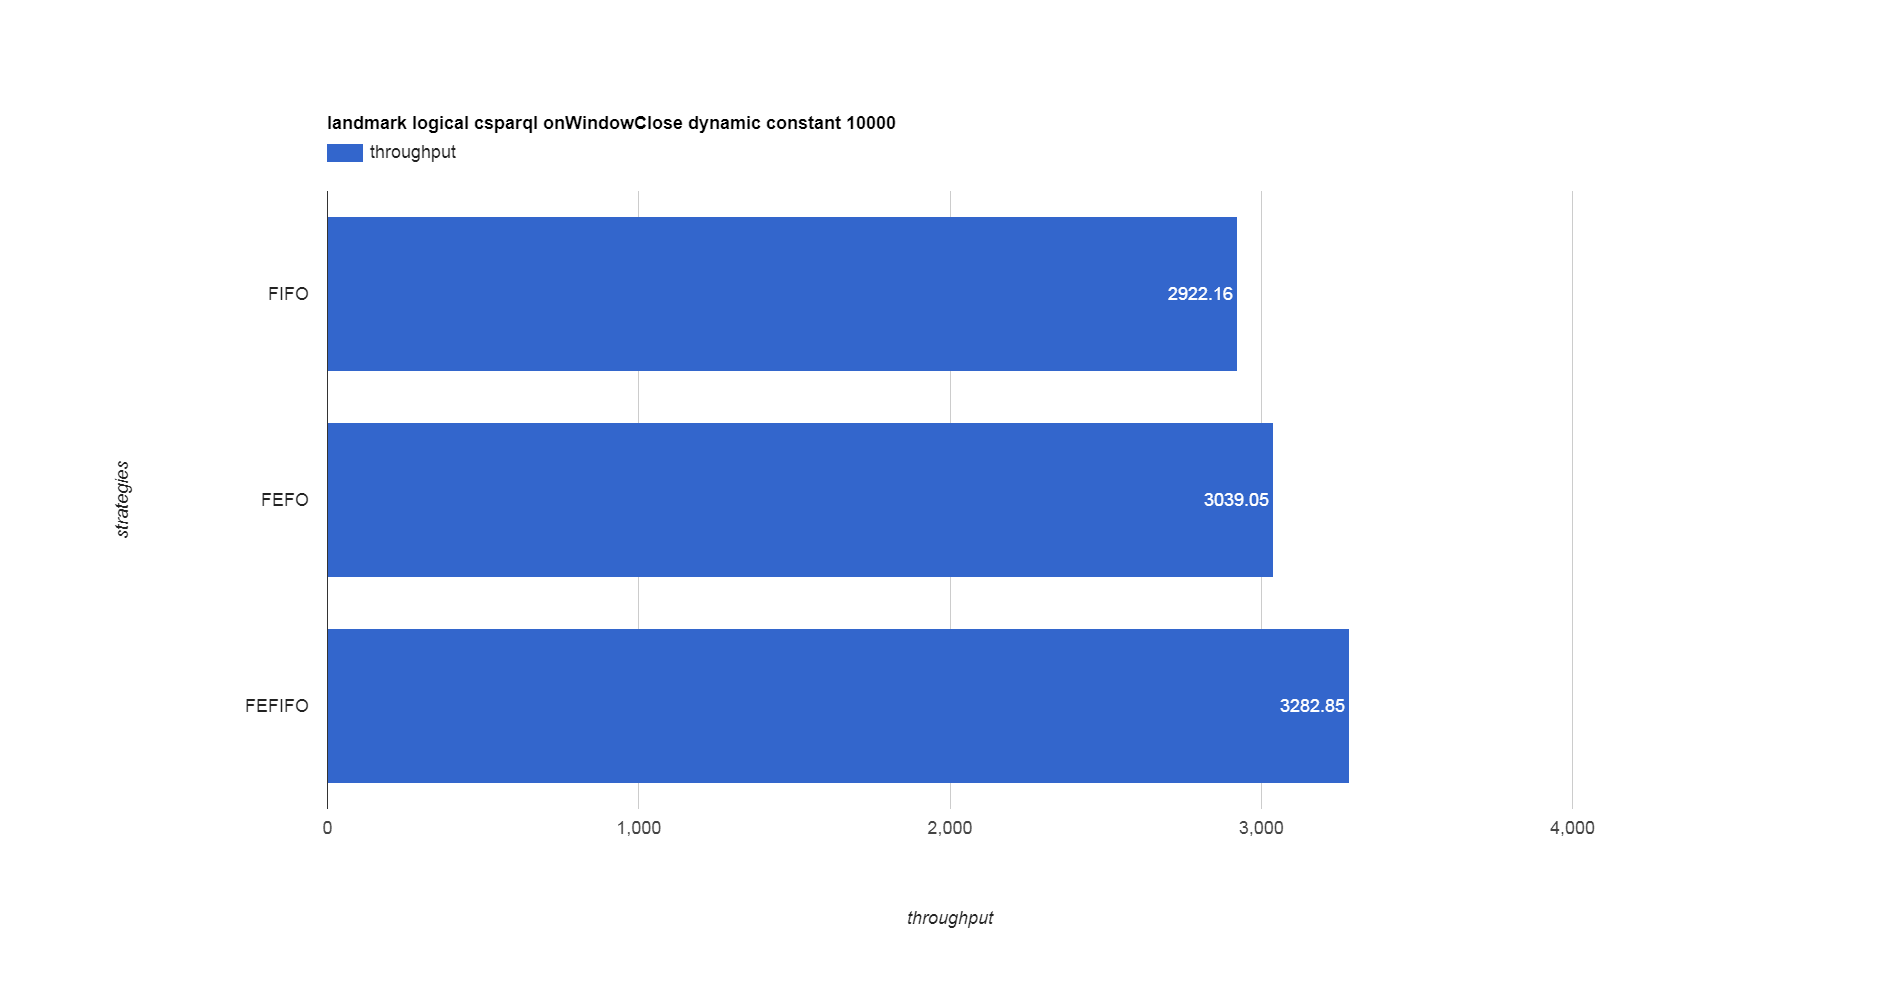
\includegraphics[width=\textwidth]{img/app3-ets-quick-t.png}
    \caption{Quick Data Expiration Throughput}
\end{figure}
\begin{figure}[!htbp]
    \centering
    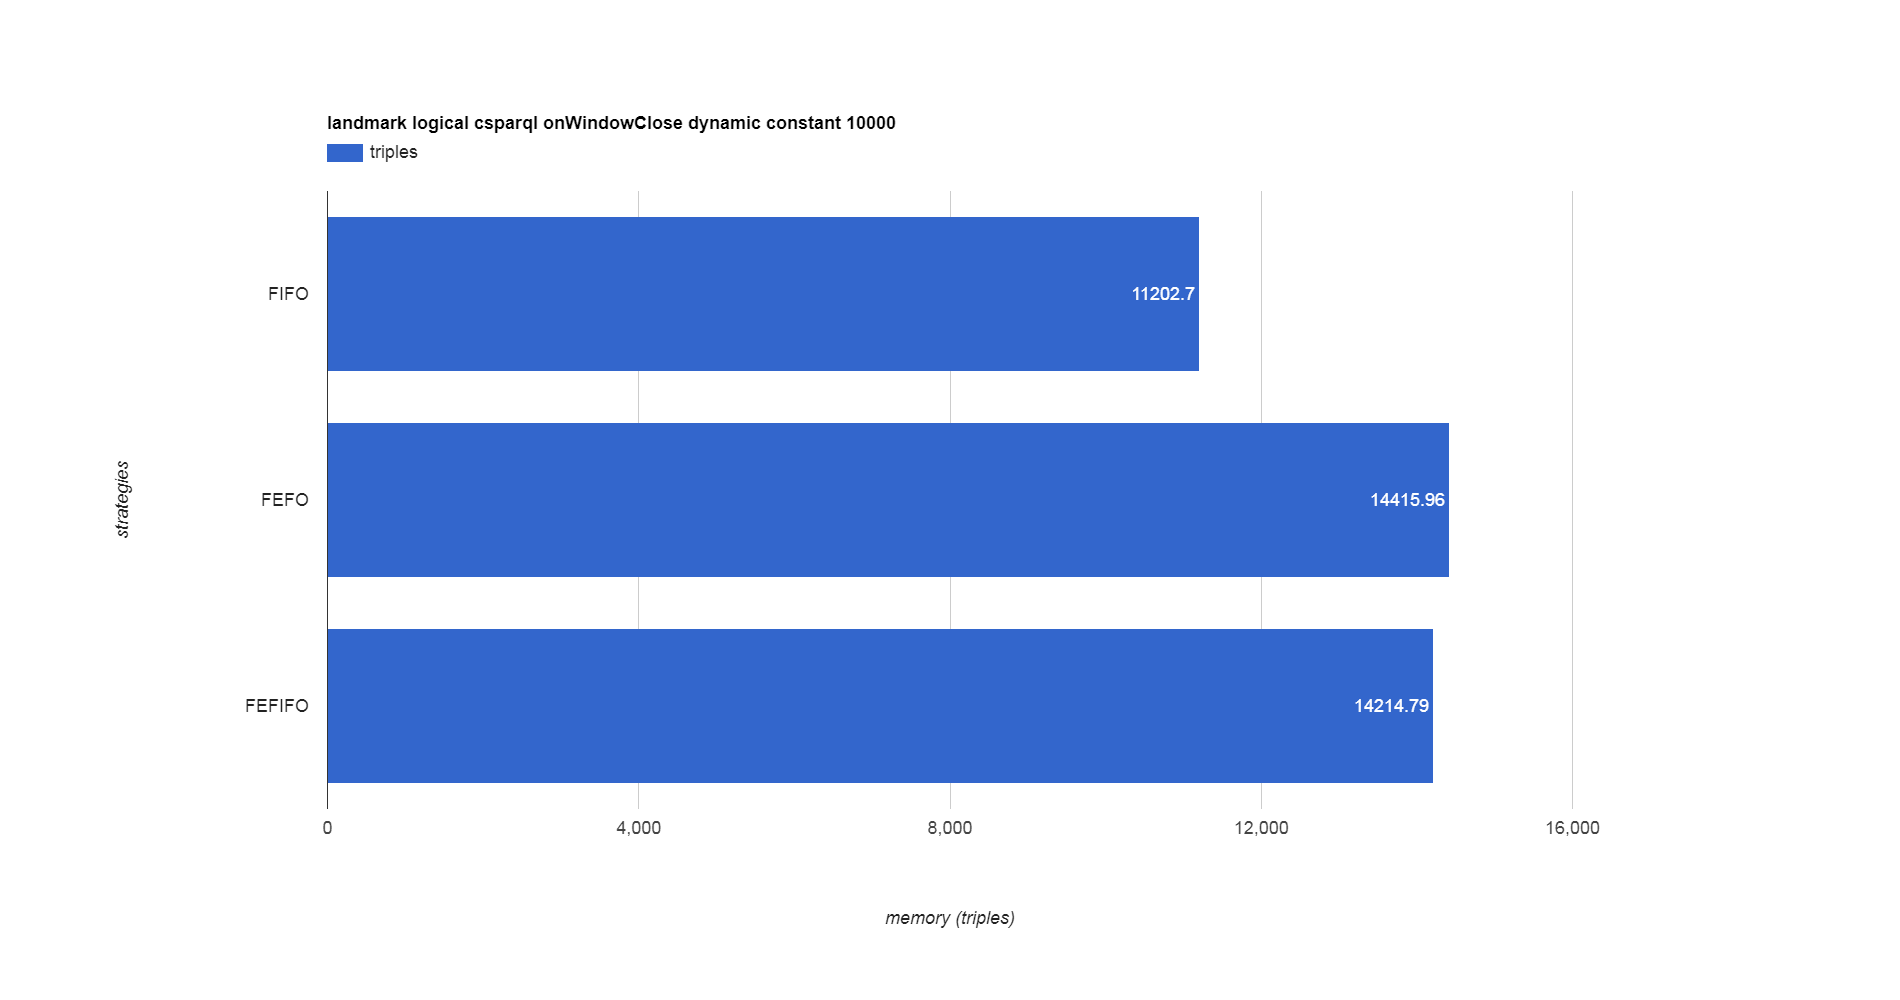
\includegraphics[width=\textwidth]{img/app3-ets-normal-m.png}
    \caption{Normal Data Expiration Memory Consumption}
\end{figure}
\begin{figure}[!htbp]
    \centering
    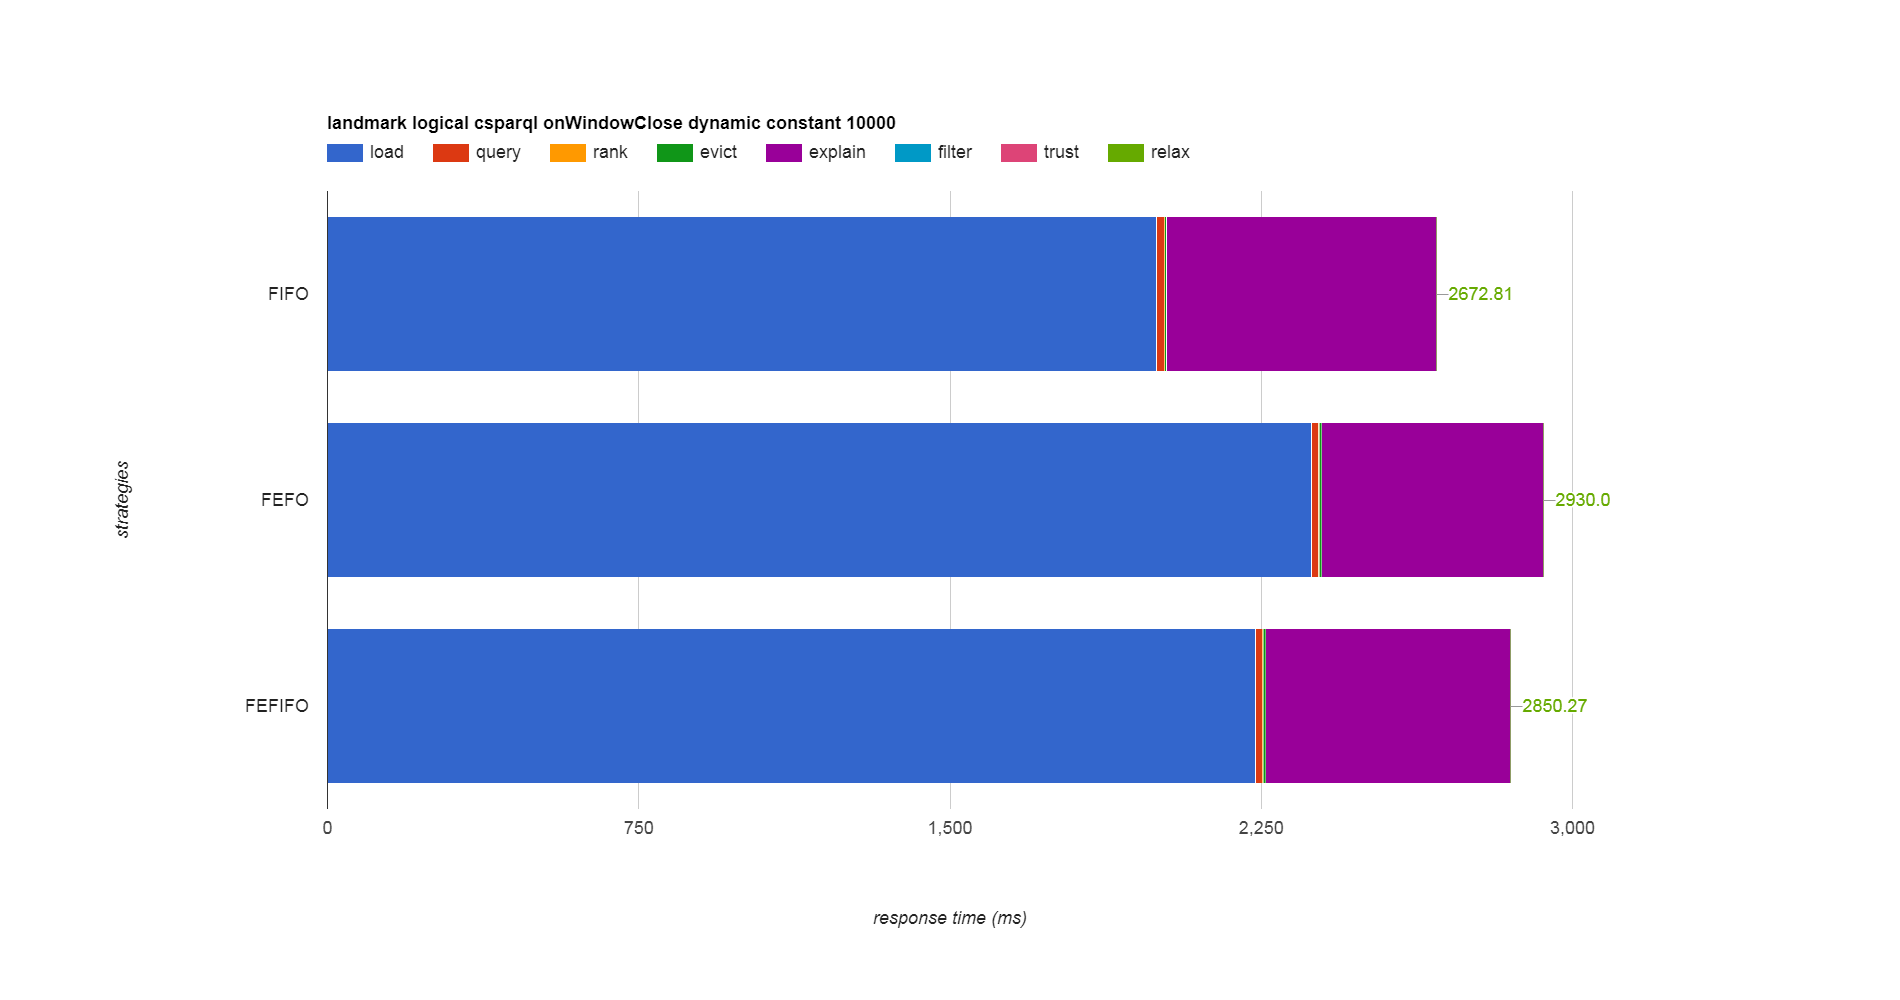
\includegraphics[width=\textwidth]{img/app3-ets-normal-r.png}
    \caption{Normal Data Expiration Response Time}
\end{figure}
\begin{figure}[!htbp]
    \centering
    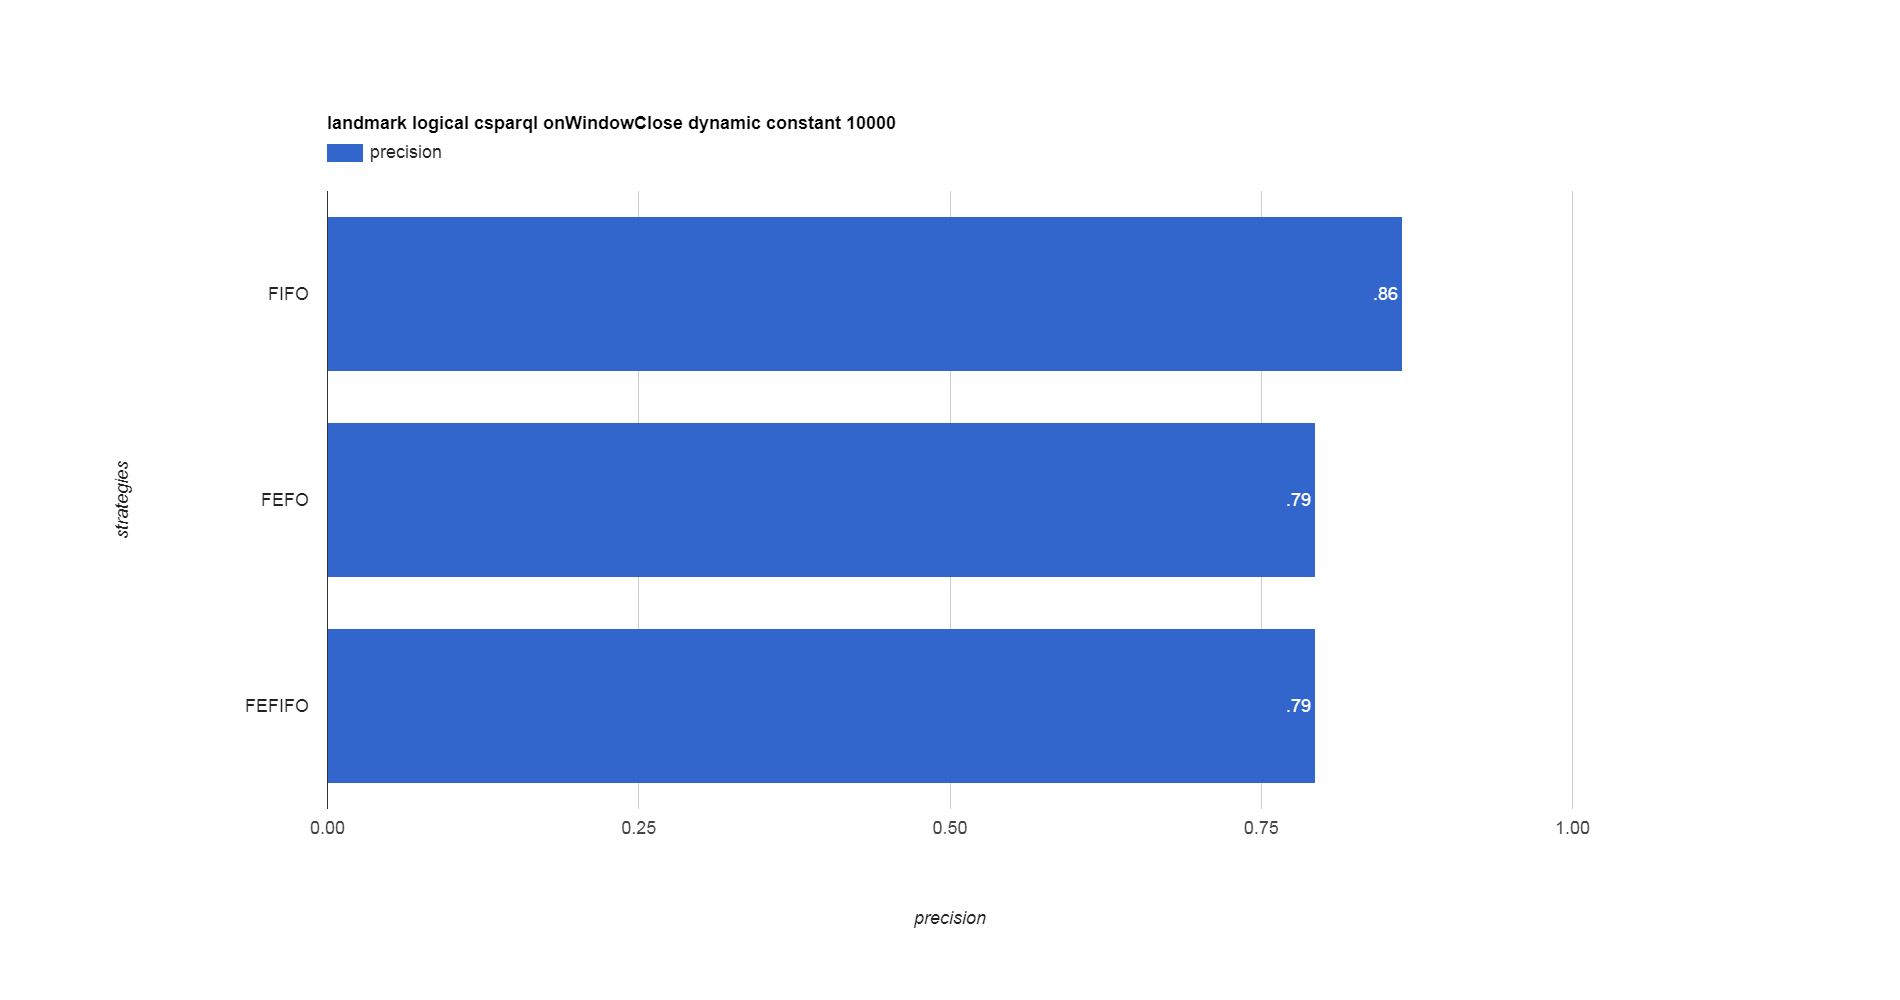
\includegraphics[width=\textwidth]{img/app3-ets-normal-p.png}
    \caption{Normal Data Expiration Precision}
\end{figure}
\begin{figure}[!htbp]
    \centering
    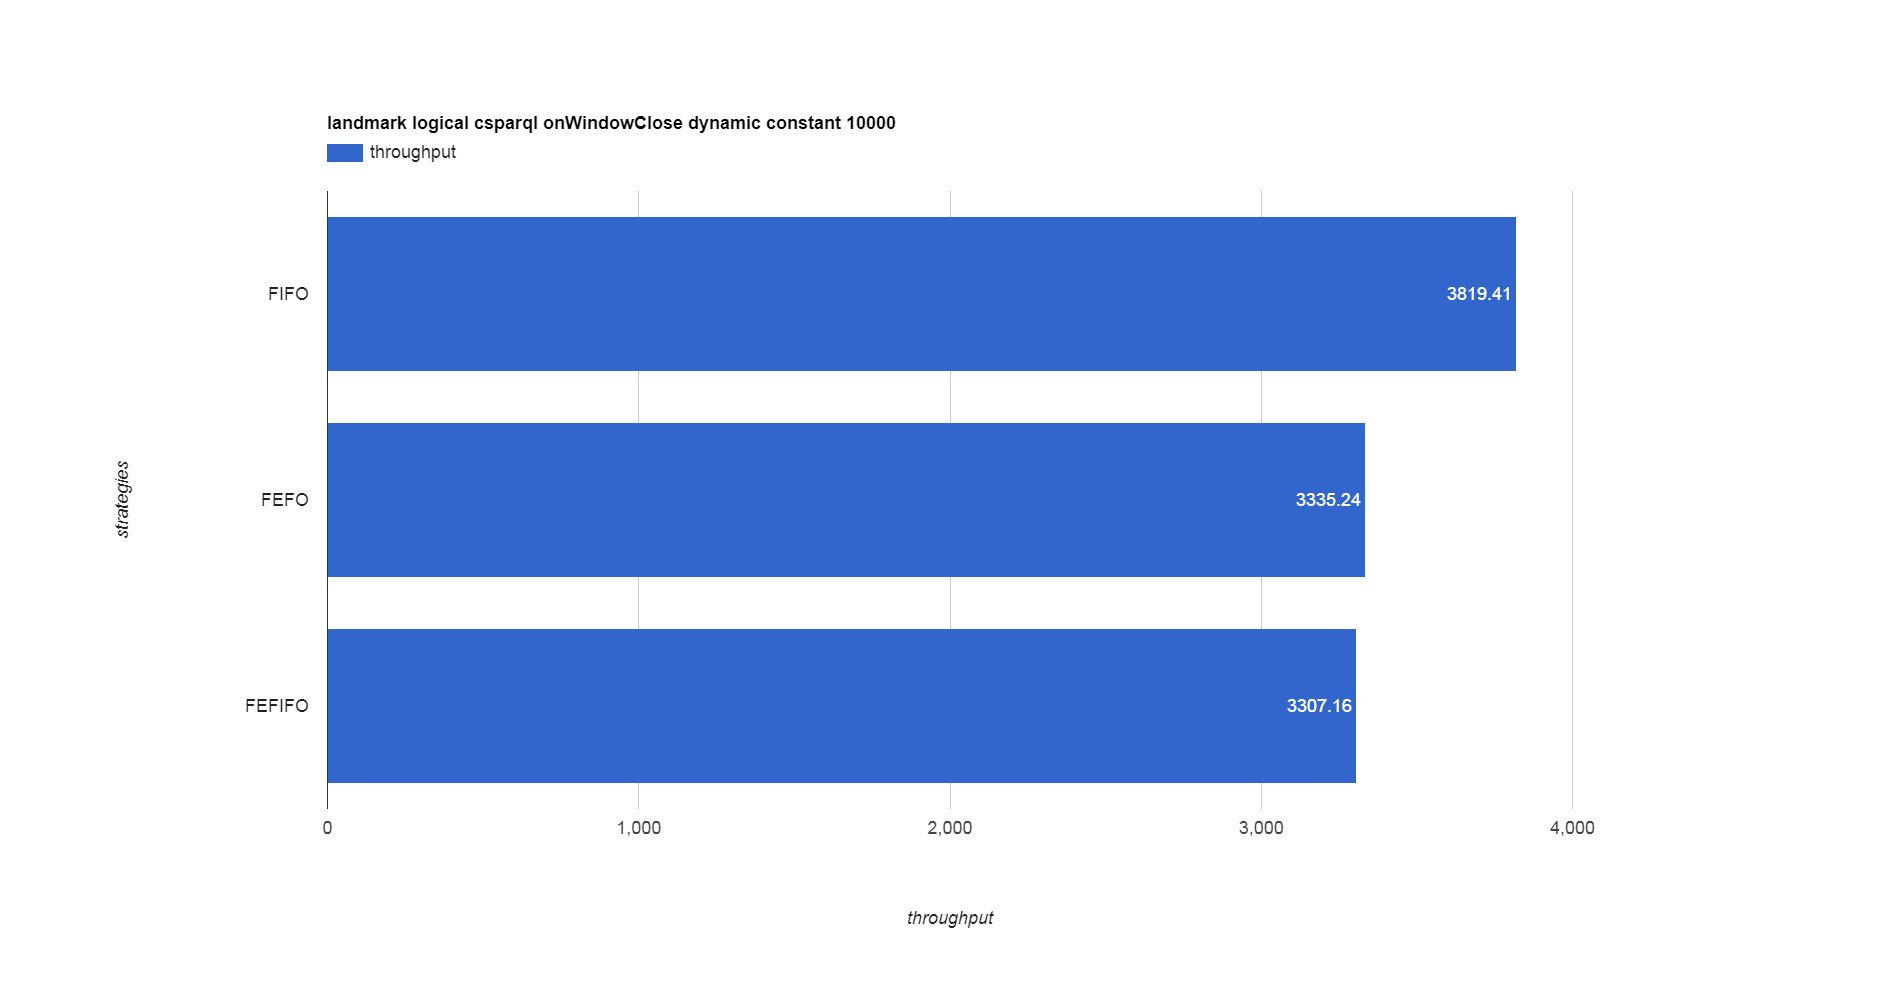
\includegraphics[width=\textwidth]{img/app3-ets-normal-t.png}
    \caption{Normal Data Expiration Throughput}
\end{figure}
\begin{figure}[!htbp]
    \centering
    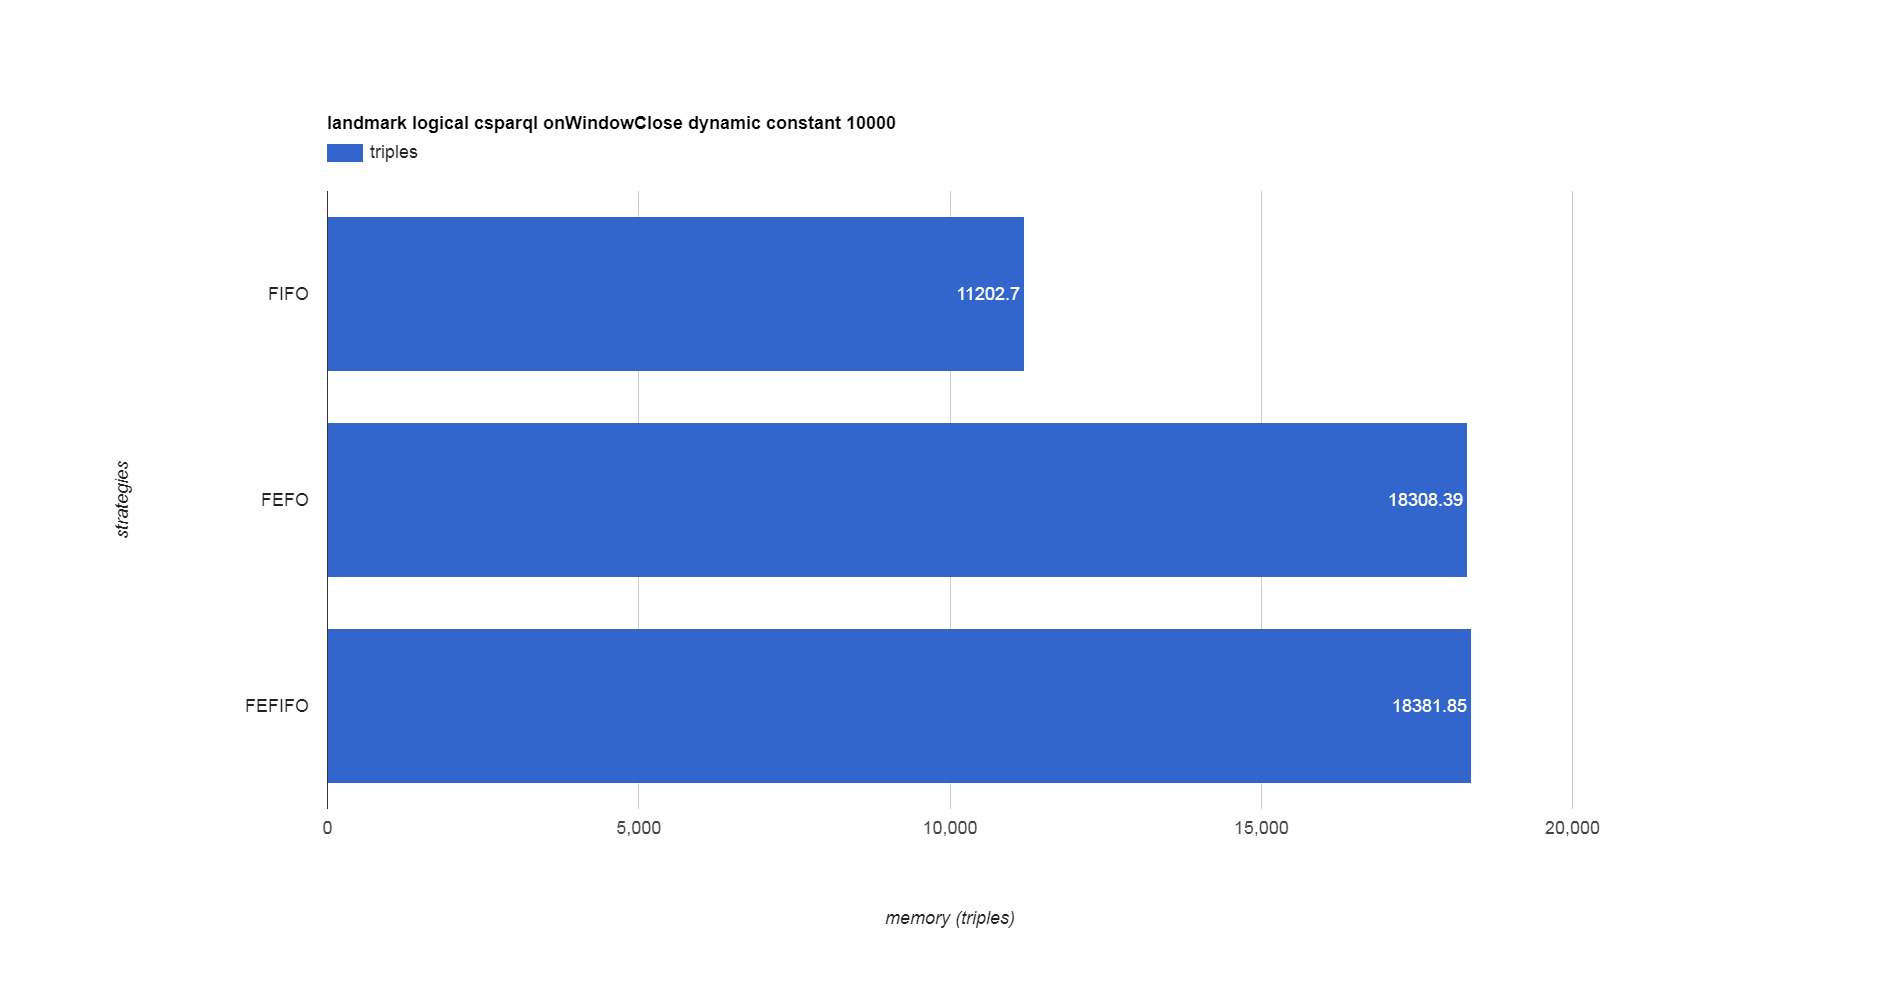
\includegraphics[width=\textwidth]{img/app3-ets-slow-m.png}
    \caption{Slow Data Expiration Memory Consumption}
\end{figure}
\begin{figure}[!htbp]
    \centering
    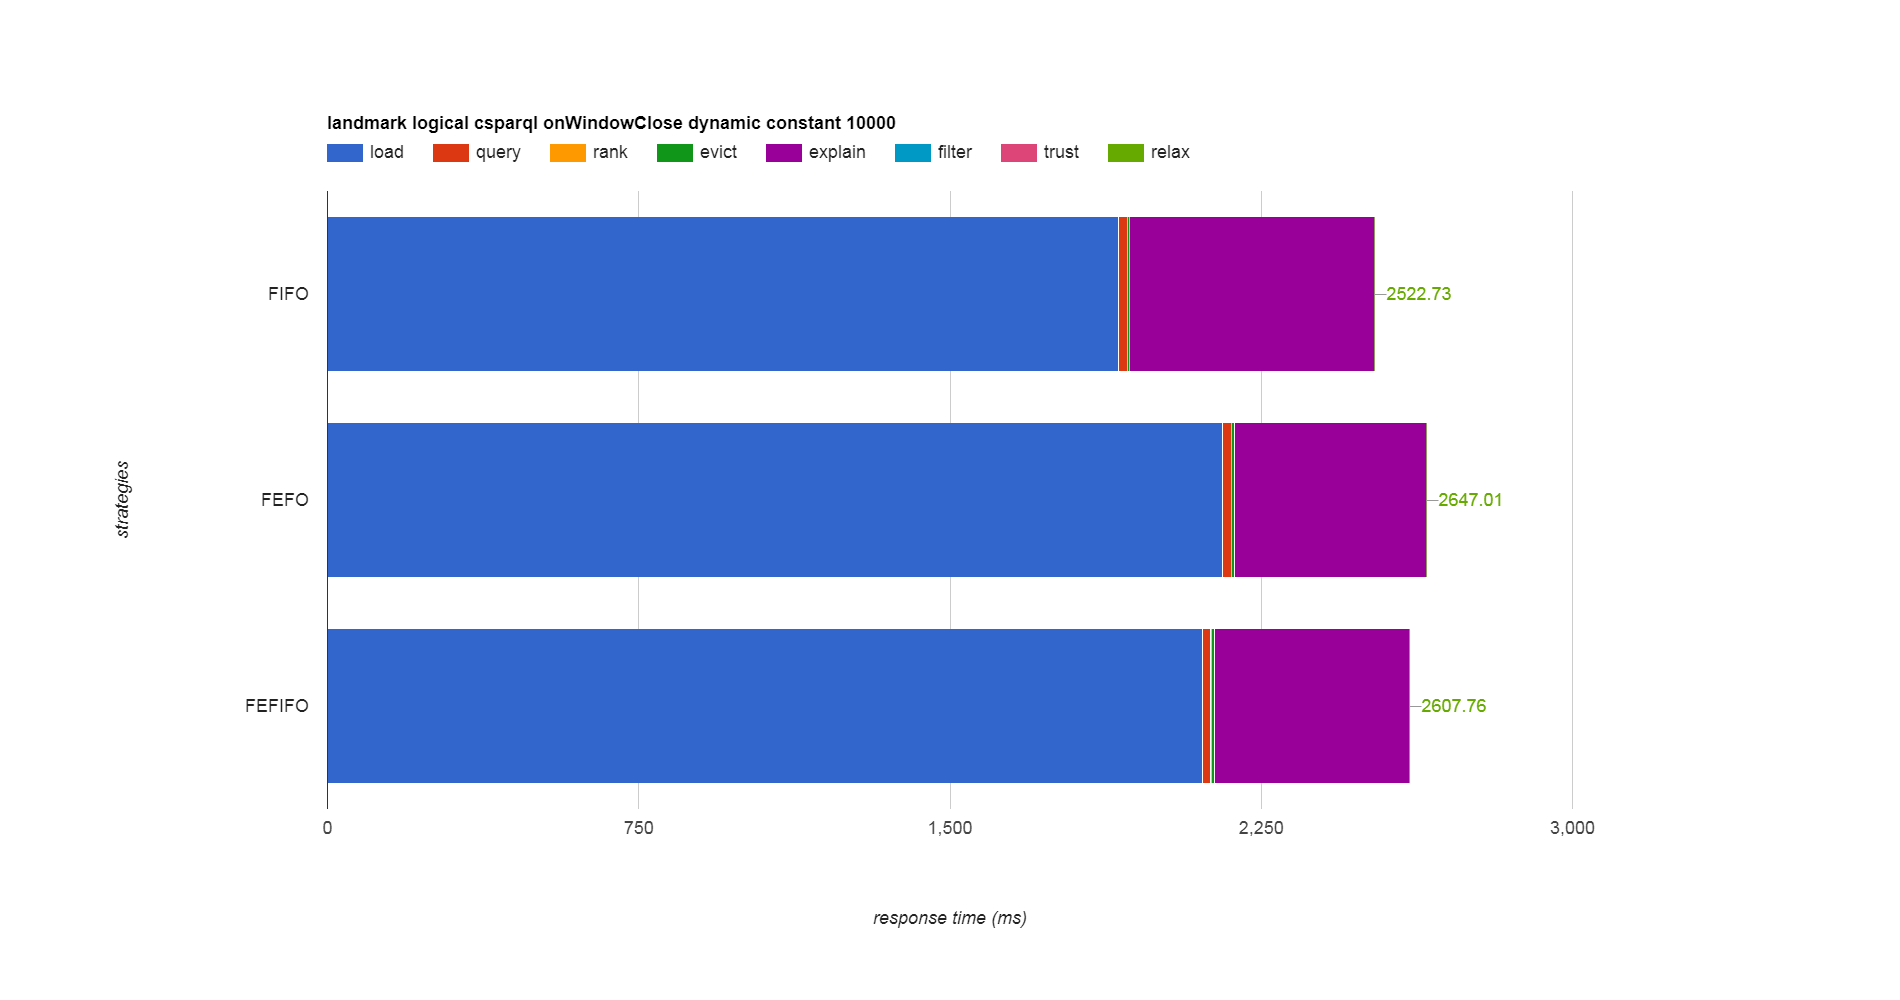
\includegraphics[width=\textwidth]{img/app3-ets-slow-r.png}
    \caption{Slow Data Expiration Response Time}
\end{figure}
\begin{figure}[!htbp]
    \centering
    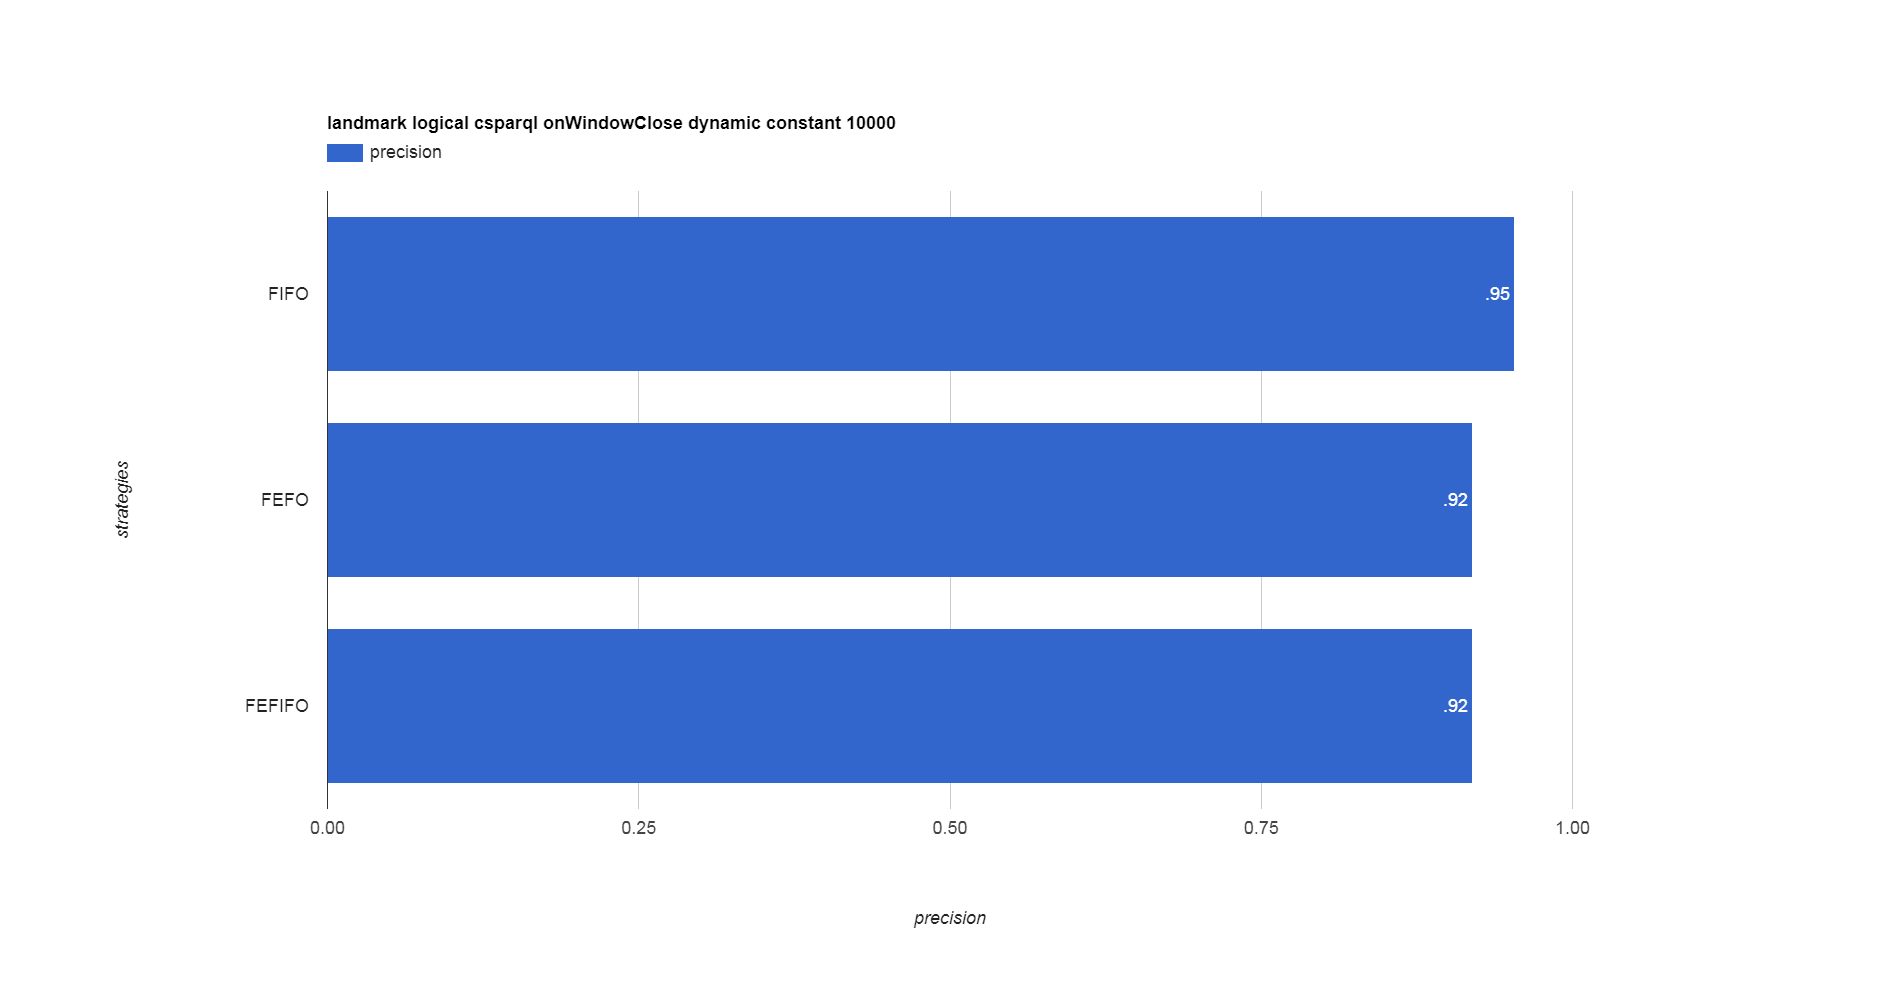
\includegraphics[width=\textwidth]{img/app3-ets-slow-p.png}
    \caption{Slow Data Expiration Precision}
\end{figure}
\begin{figure}[!htbp]
    \centering
    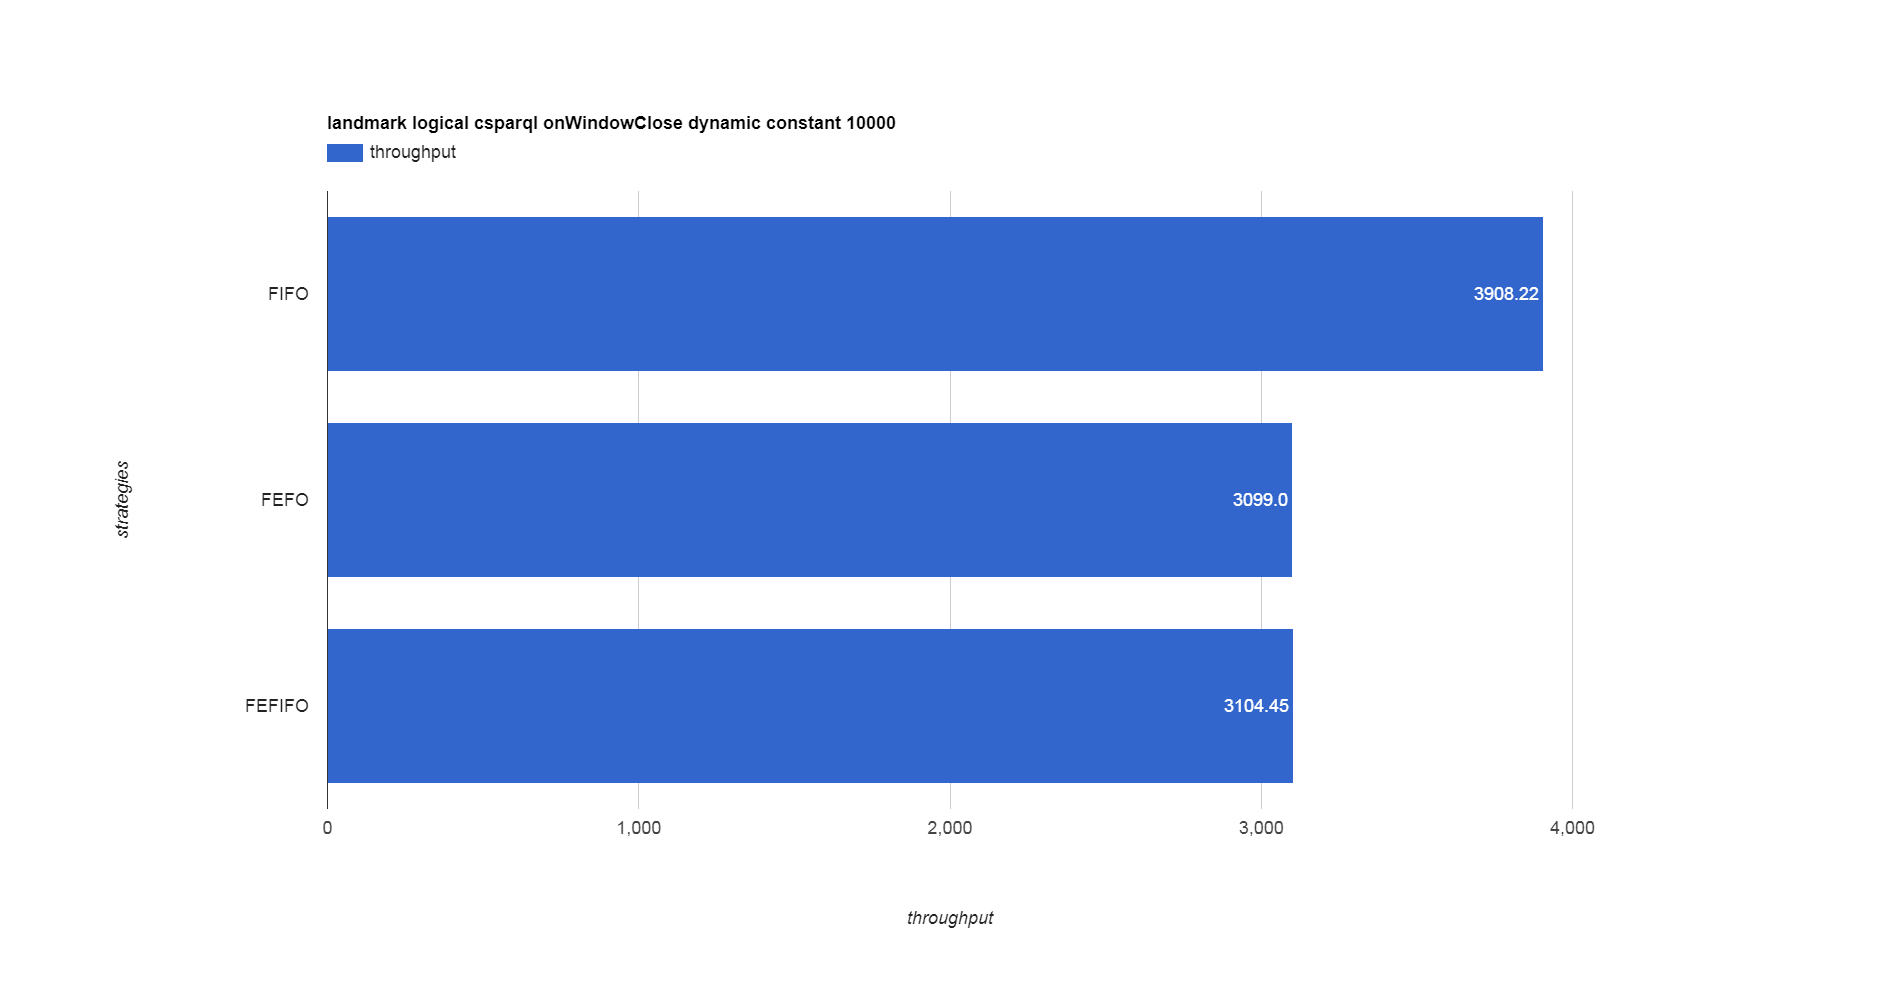
\includegraphics[width=\textwidth]{img/app3-ets-slow-t.png}
    \caption{Slow Data Expiration Throughput}
\end{figure}
%%%%%%%%%%%%%%%%%%%%%%%%%
%%%%%%%%%%%%%%%%%%%%%%%%%
%% query participation %%
%%%%%%%%%%%%%%%%%%%%%%%%%
%%%%%%%%%%%%%%%%%%%%%%%%%
\begin{figure}[!htbp]
    \centering
    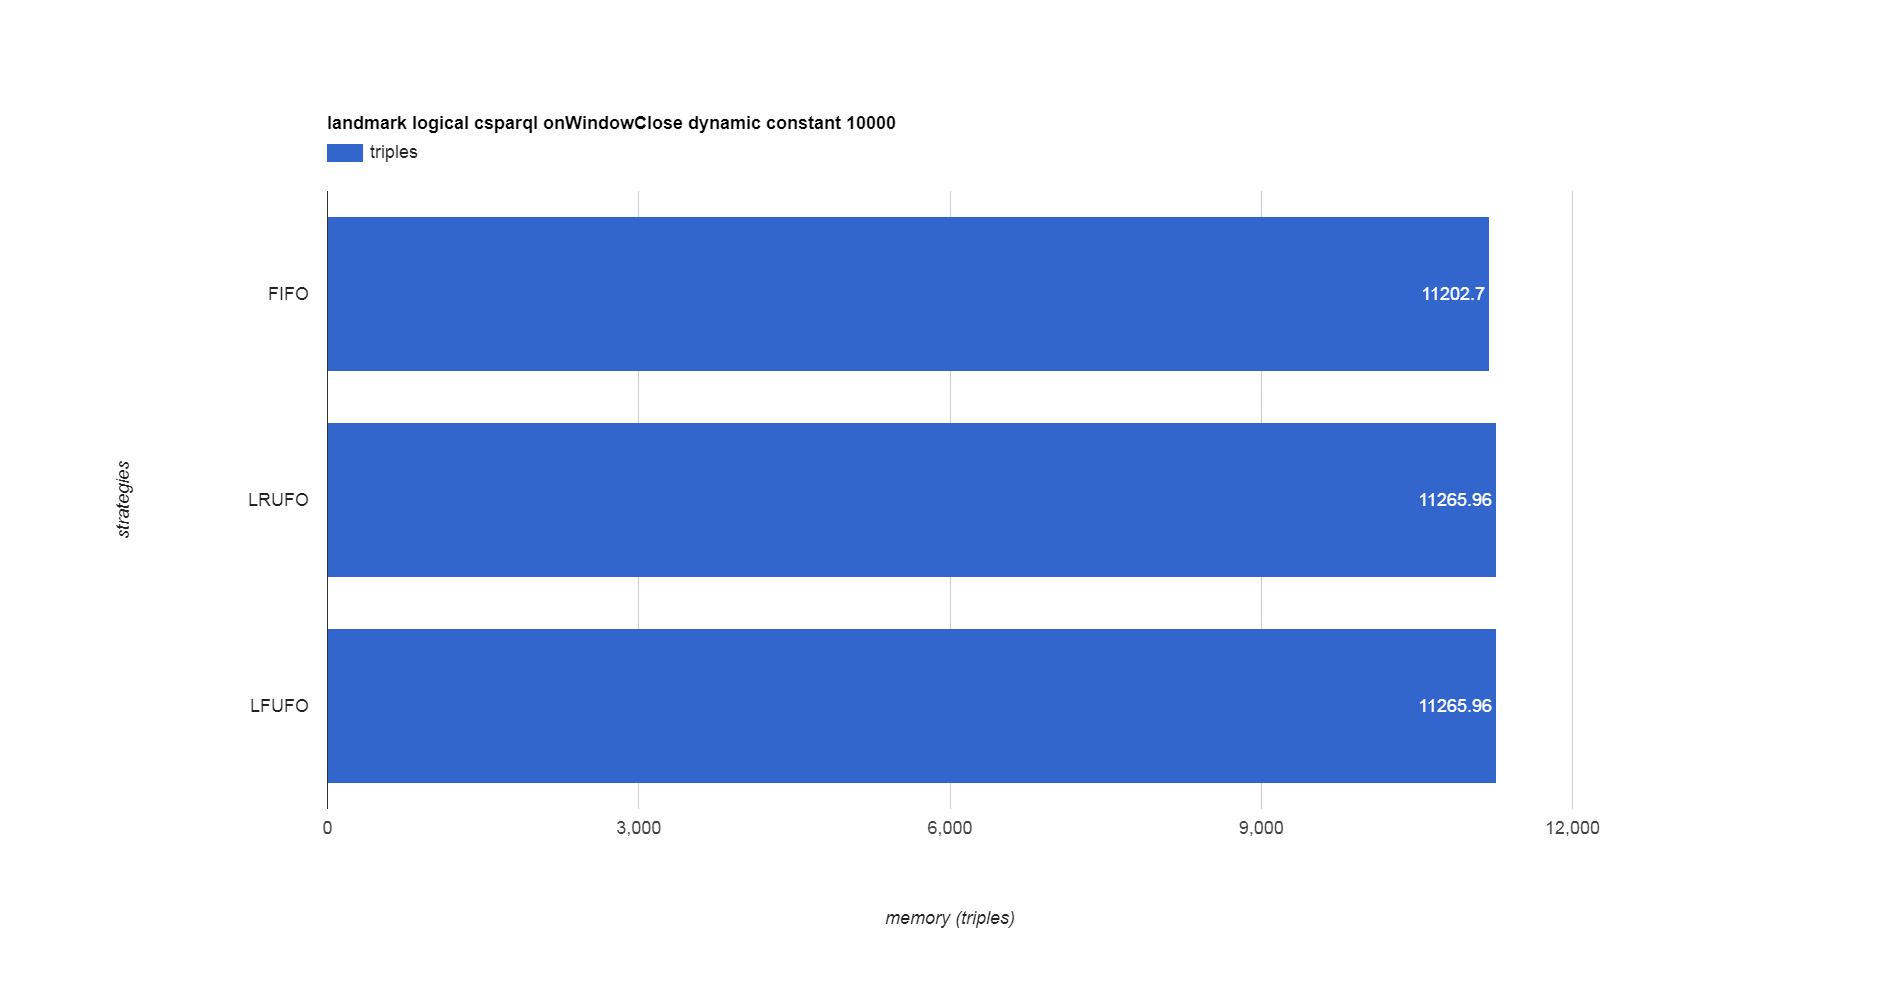
\includegraphics[width=\textwidth]{img/app3-qp-quick-m.png}
    \caption{Query Participation Quick Data Expiration Memory Consumption}
\end{figure}
\begin{figure}[!htbp]
    \centering
    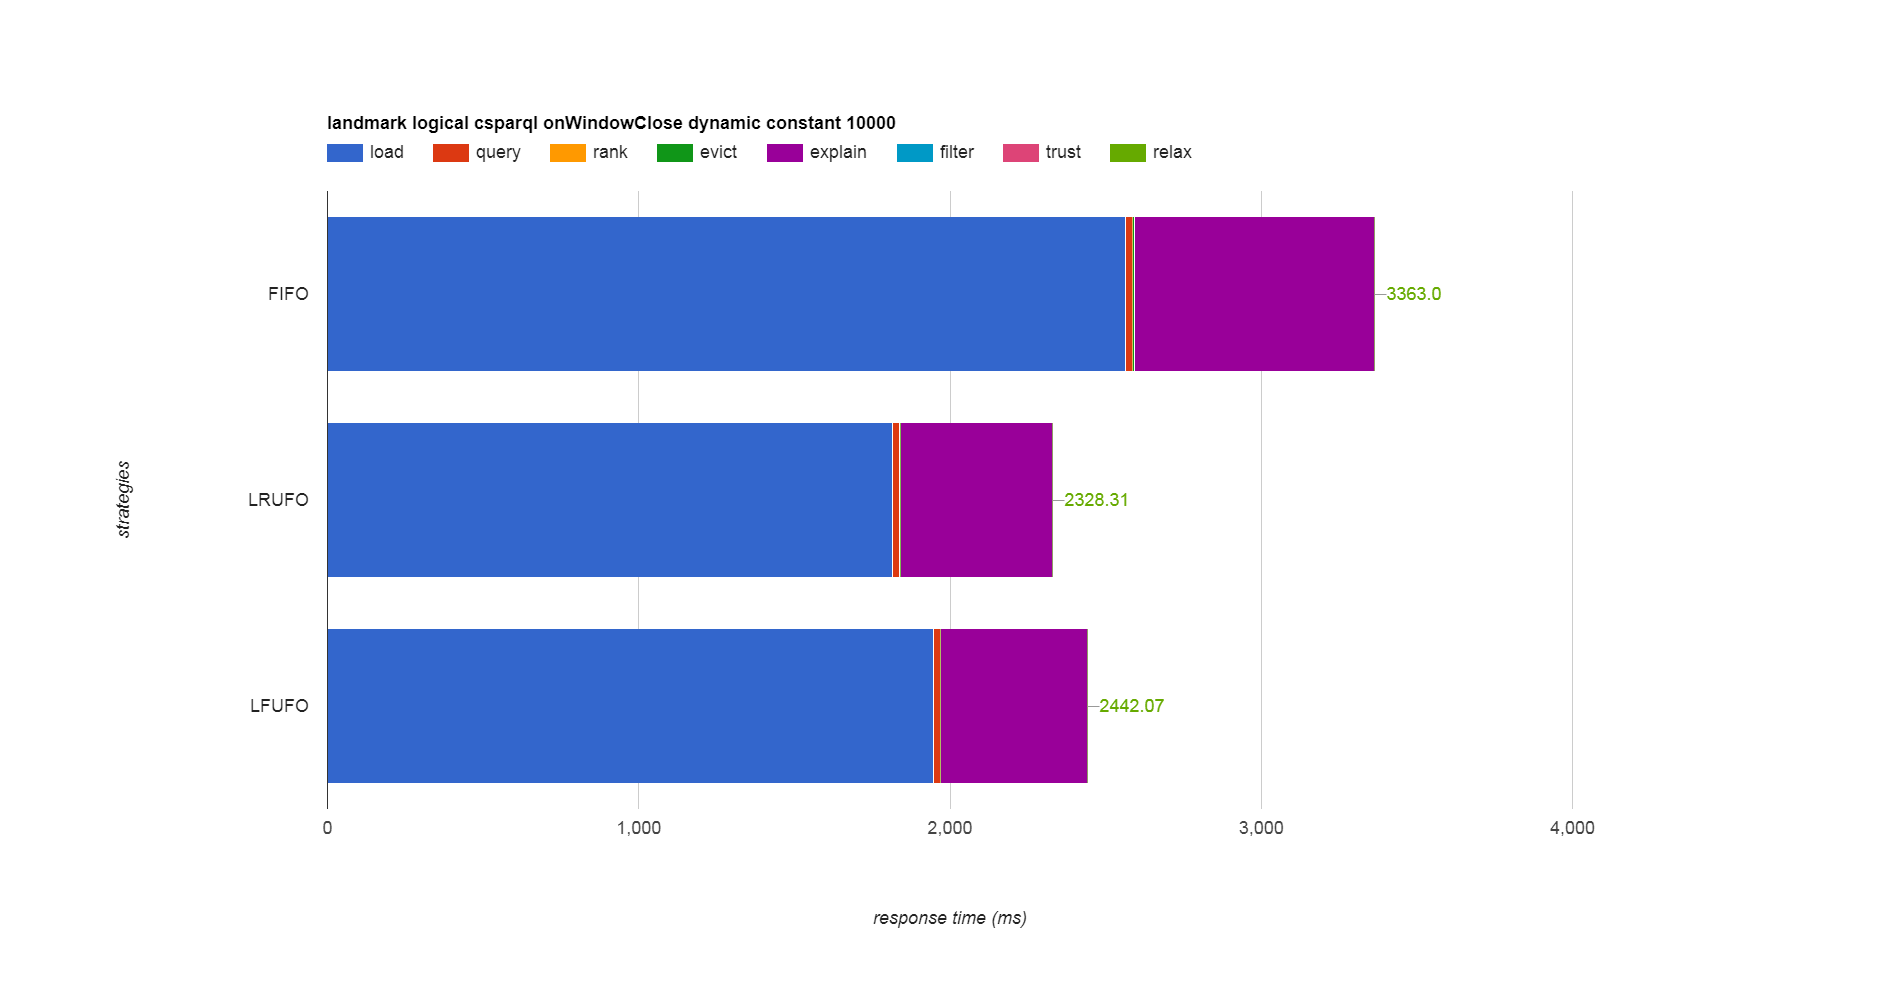
\includegraphics[width=\textwidth]{img/app3-qp-quick-r.png}
    \caption{Query Participation Quick Data Expiration Response Time}
\end{figure}
\begin{figure}[!htbp]
    \centering
    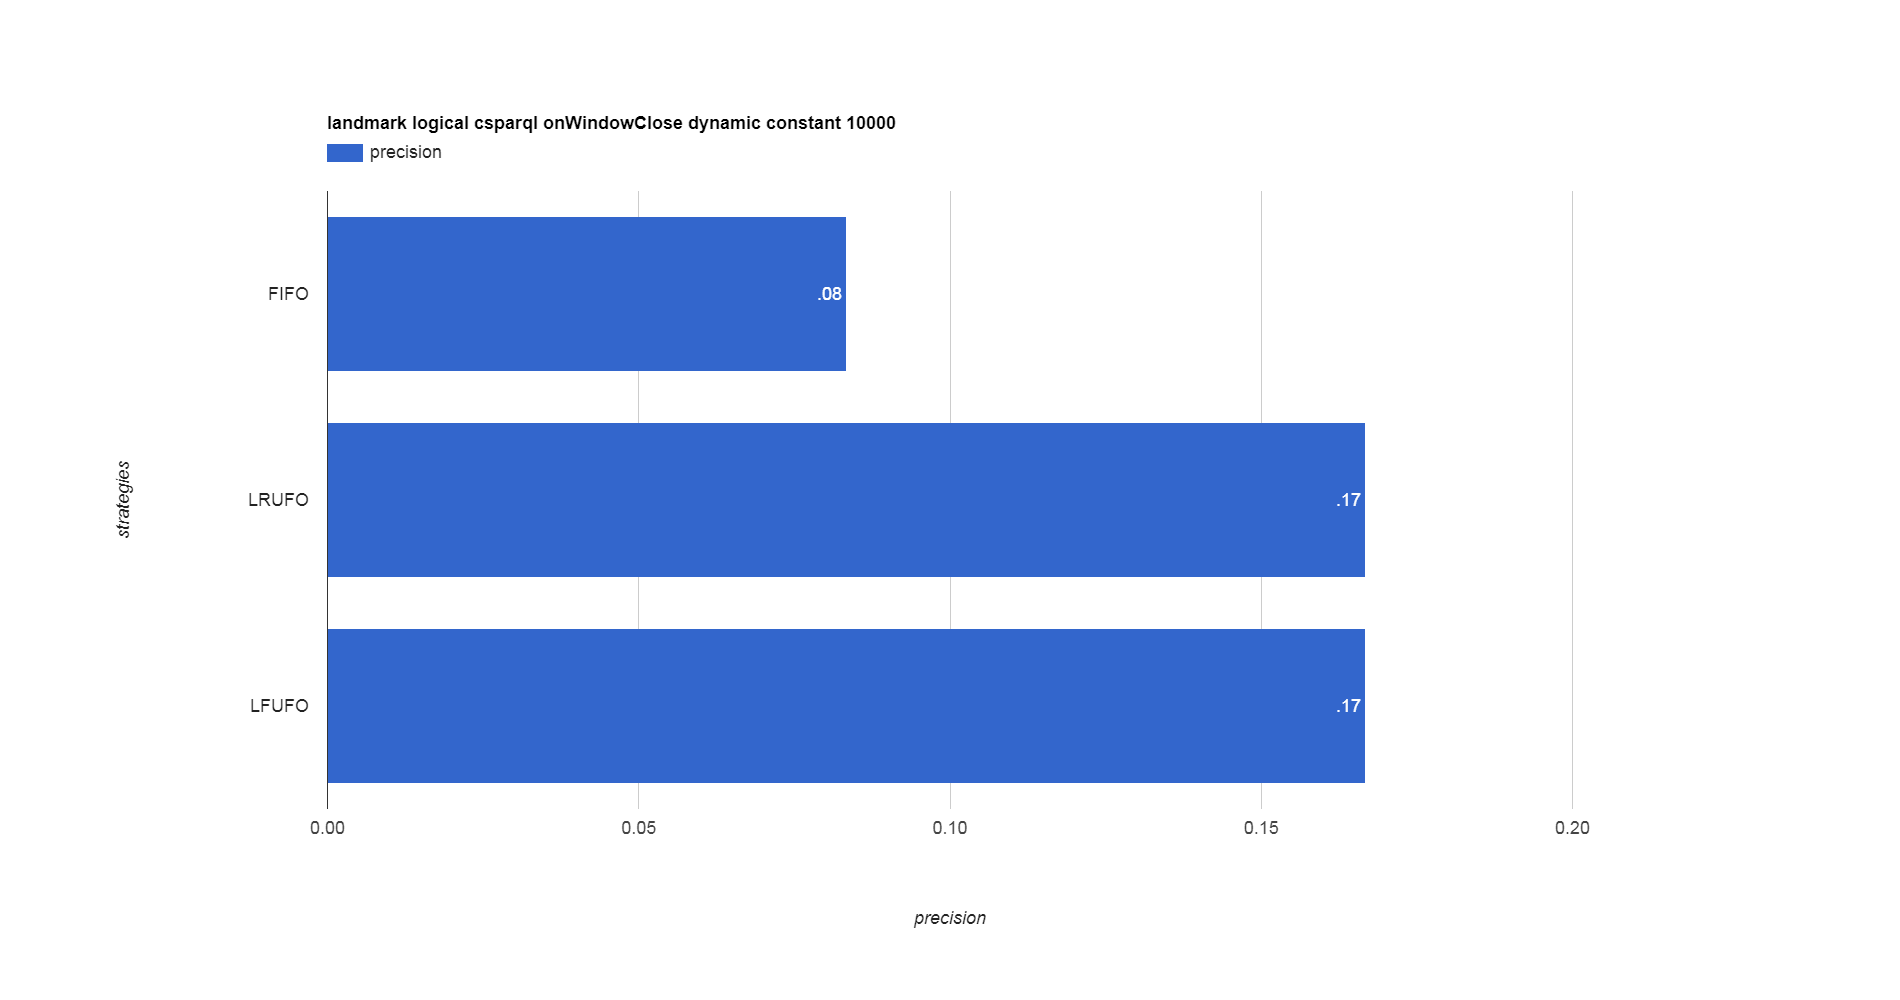
\includegraphics[width=\textwidth]{img/app3-qp-quick-p.png}
    \caption{Query Participation Quick Data Expiration Precision}
\end{figure}
\begin{figure}[!htbp]
    \centering
    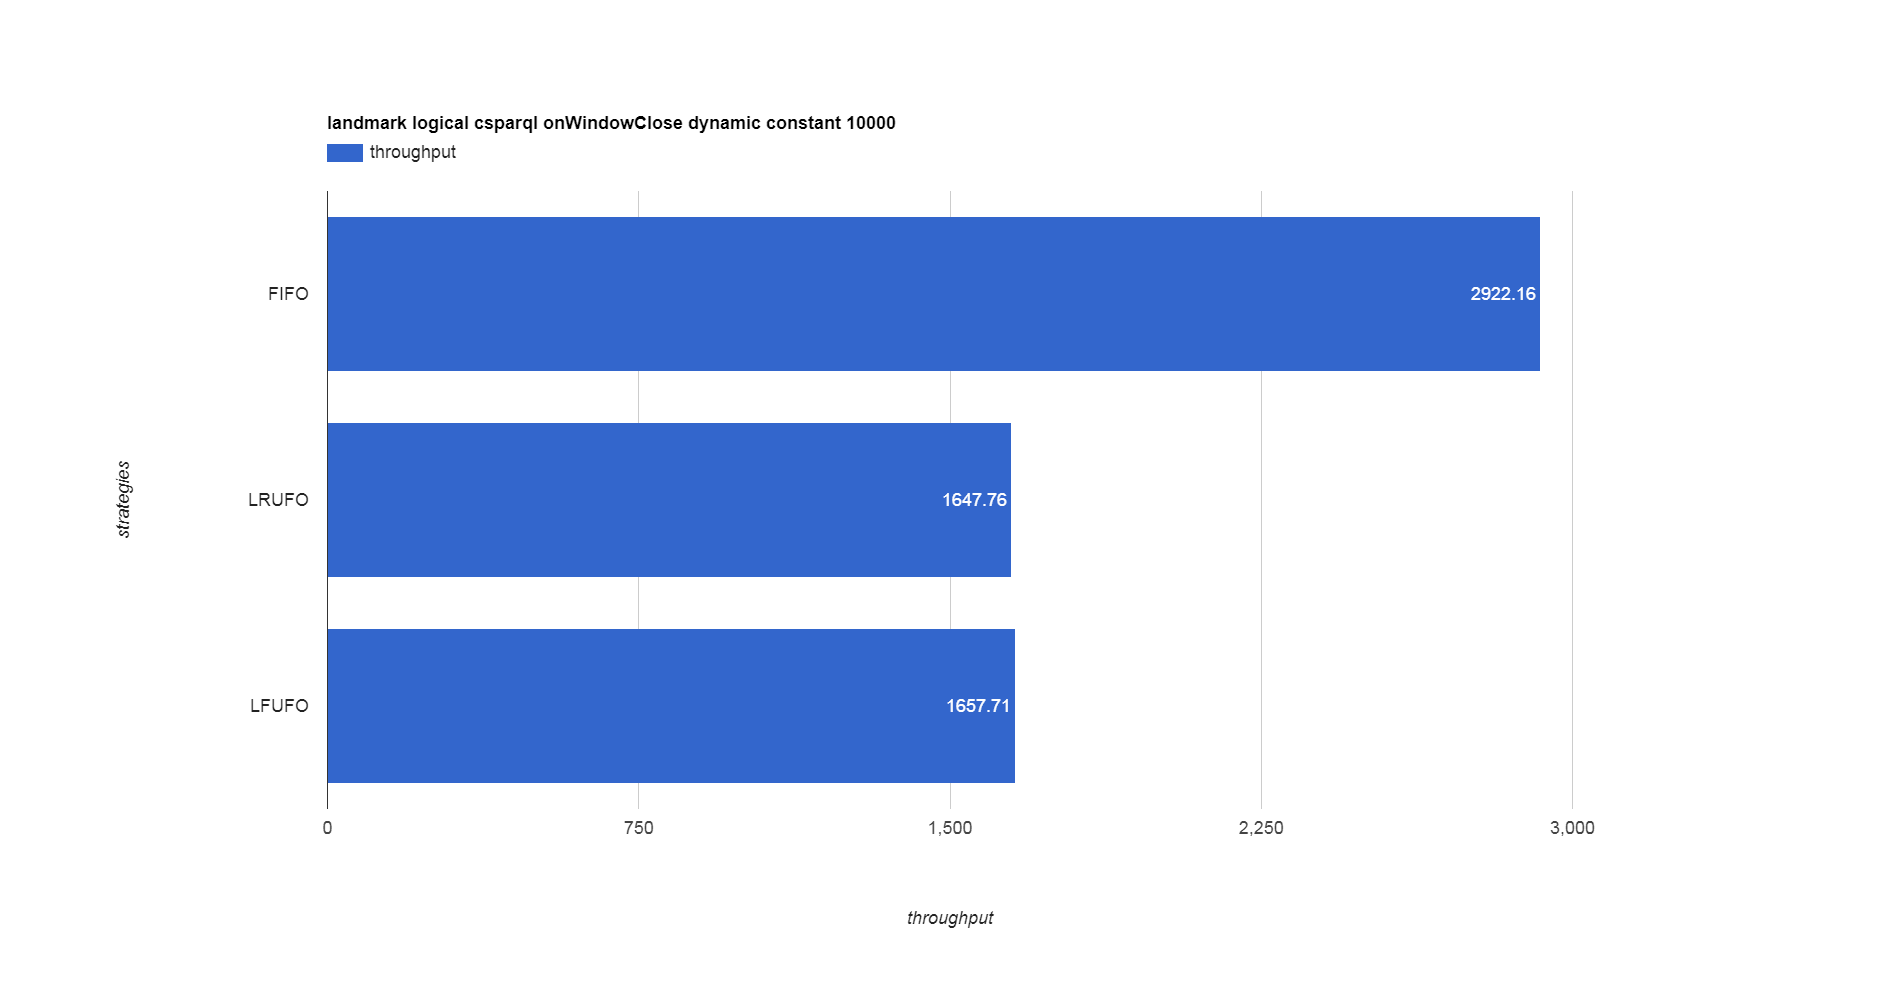
\includegraphics[width=\textwidth]{img/app3-qp-quick-t.png}
    \caption{Query Participation Quick Data Expiration Throughput}
\end{figure}
\begin{figure}[!htbp]
    \centering
    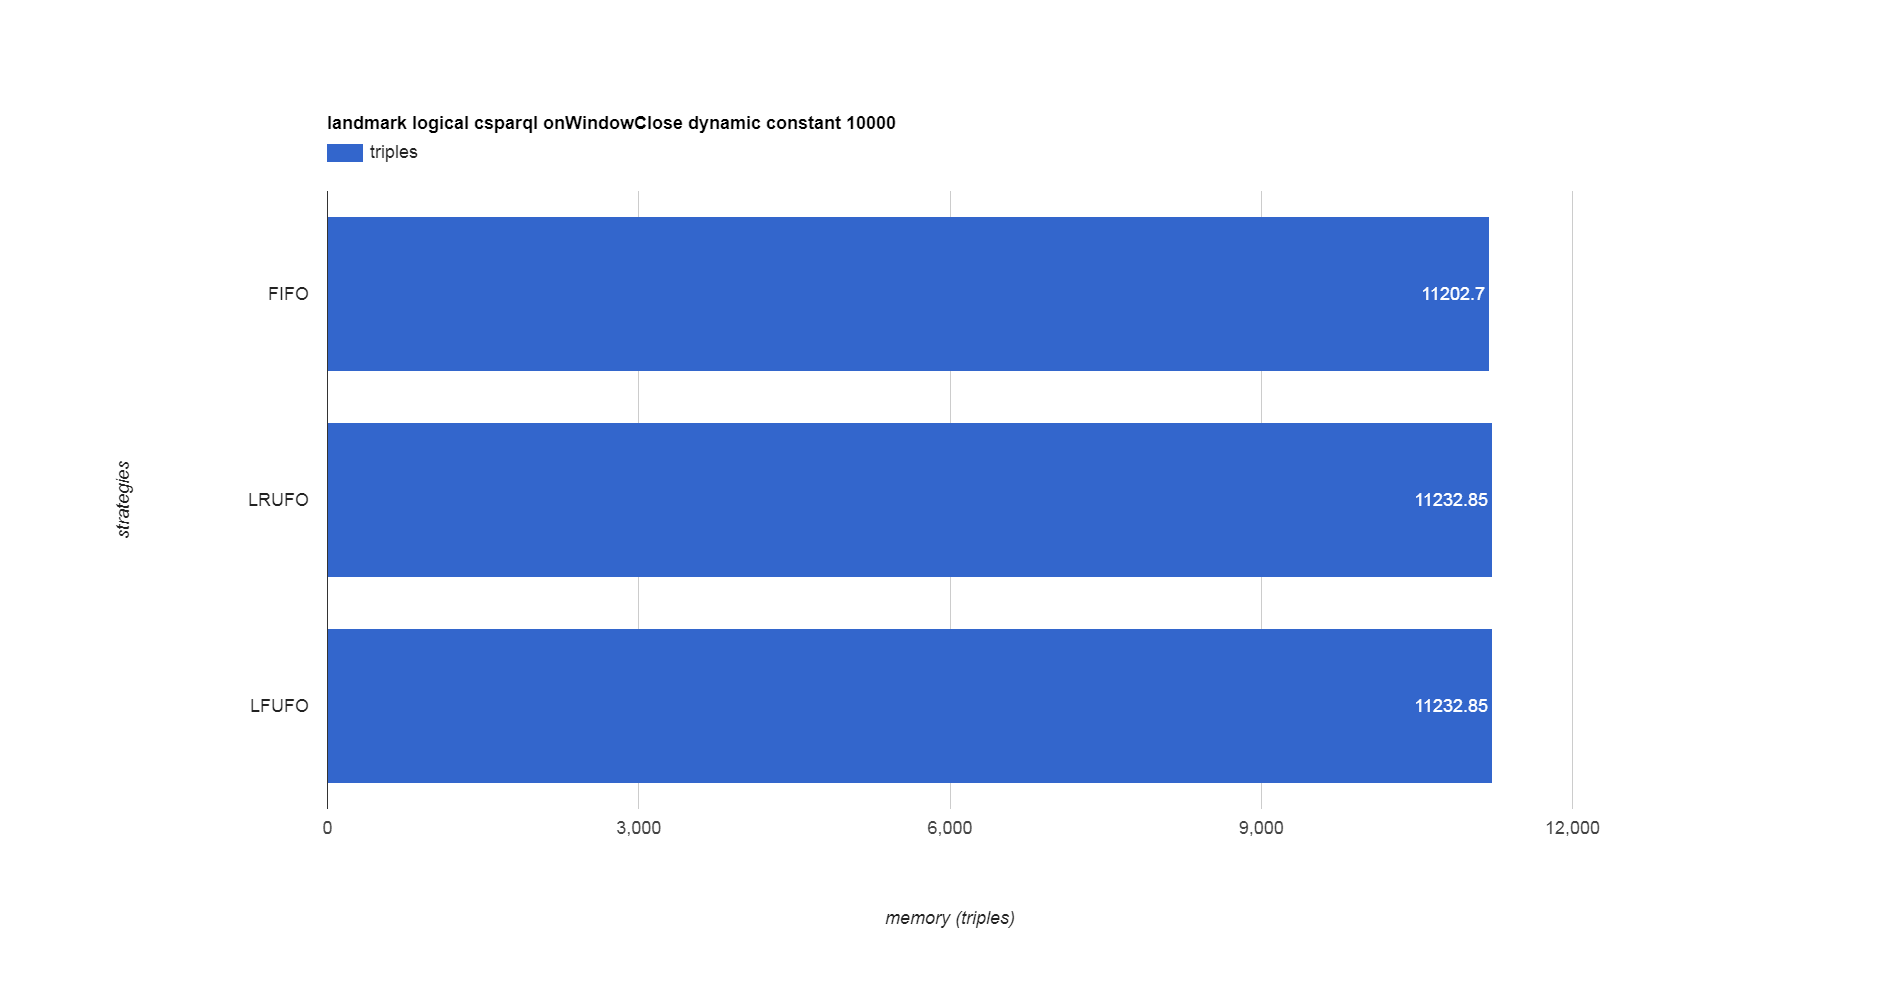
\includegraphics[width=\textwidth]{img/app3-qp-normal-m.png}
    \caption{Query Participation Normal Data Expiration Memory Consumption}
\end{figure}
\begin{figure}[!htbp]
    \centering
    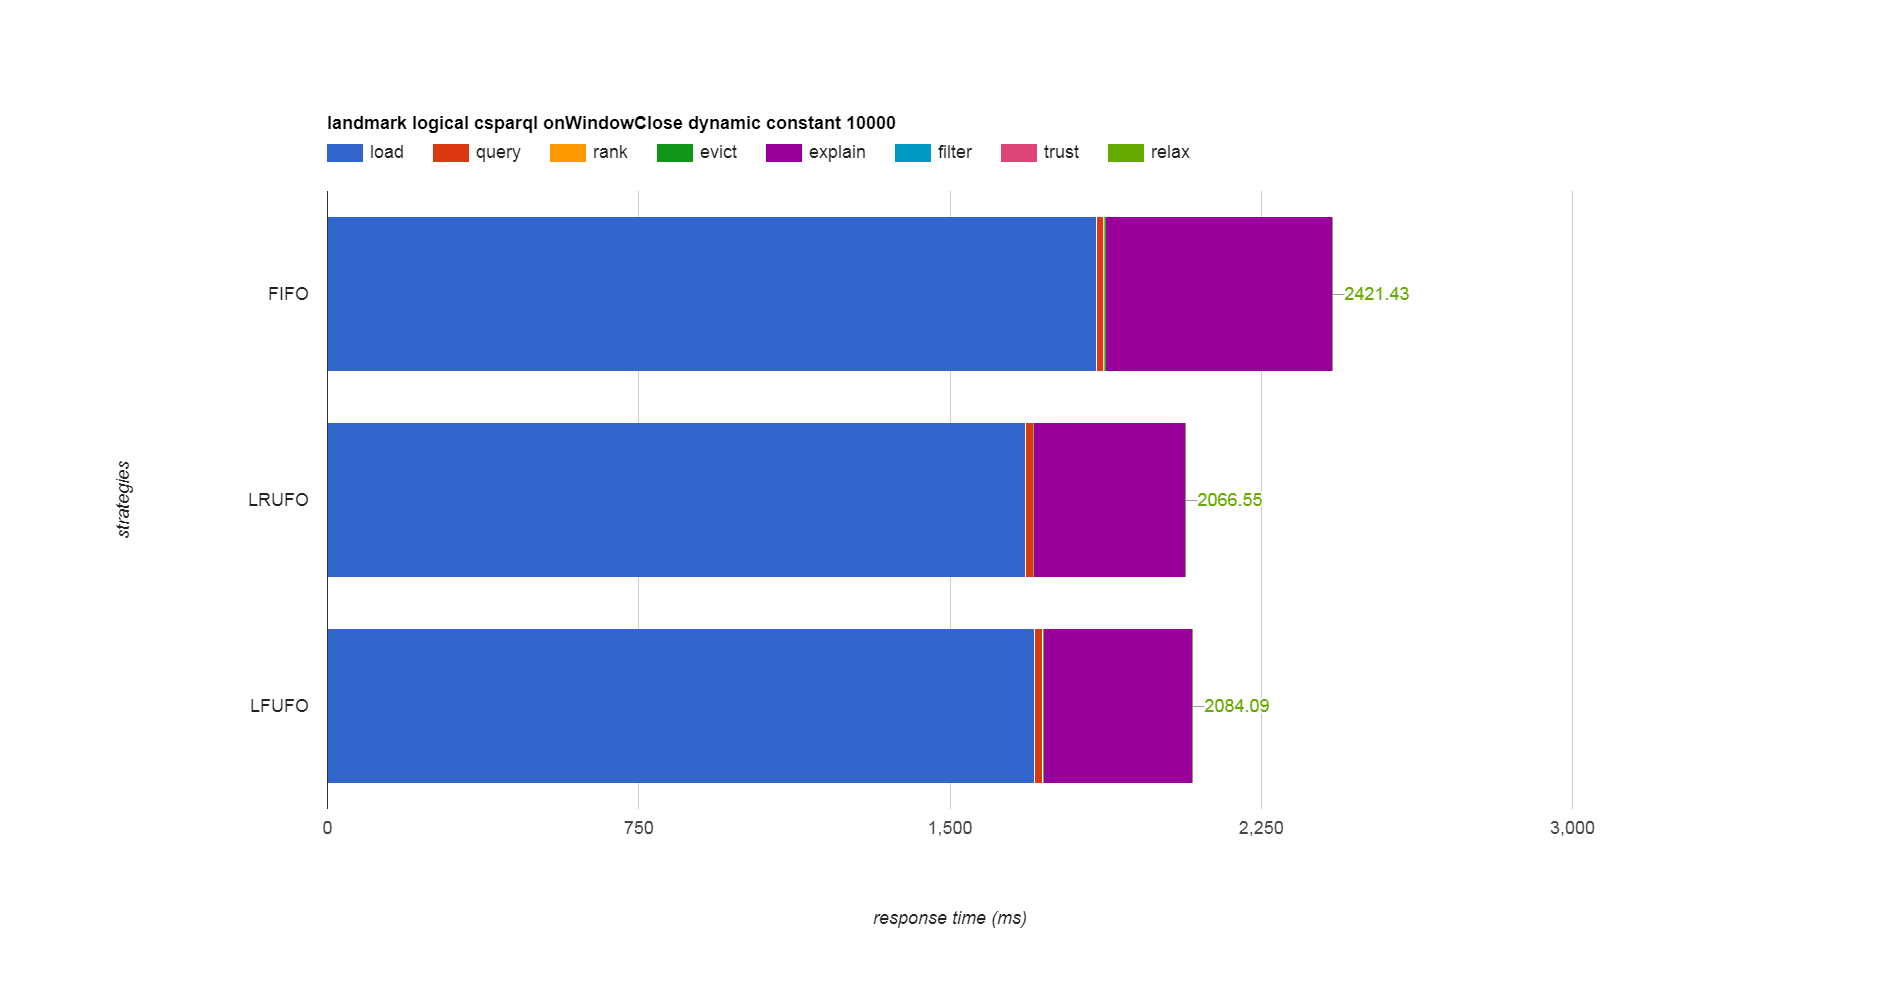
\includegraphics[width=\textwidth]{img/app3-qp-normal-r.png}
    \caption{Query Participation Normal Data Expiration Response Time}
\end{figure}
\begin{figure}[!htbp]
    \centering
    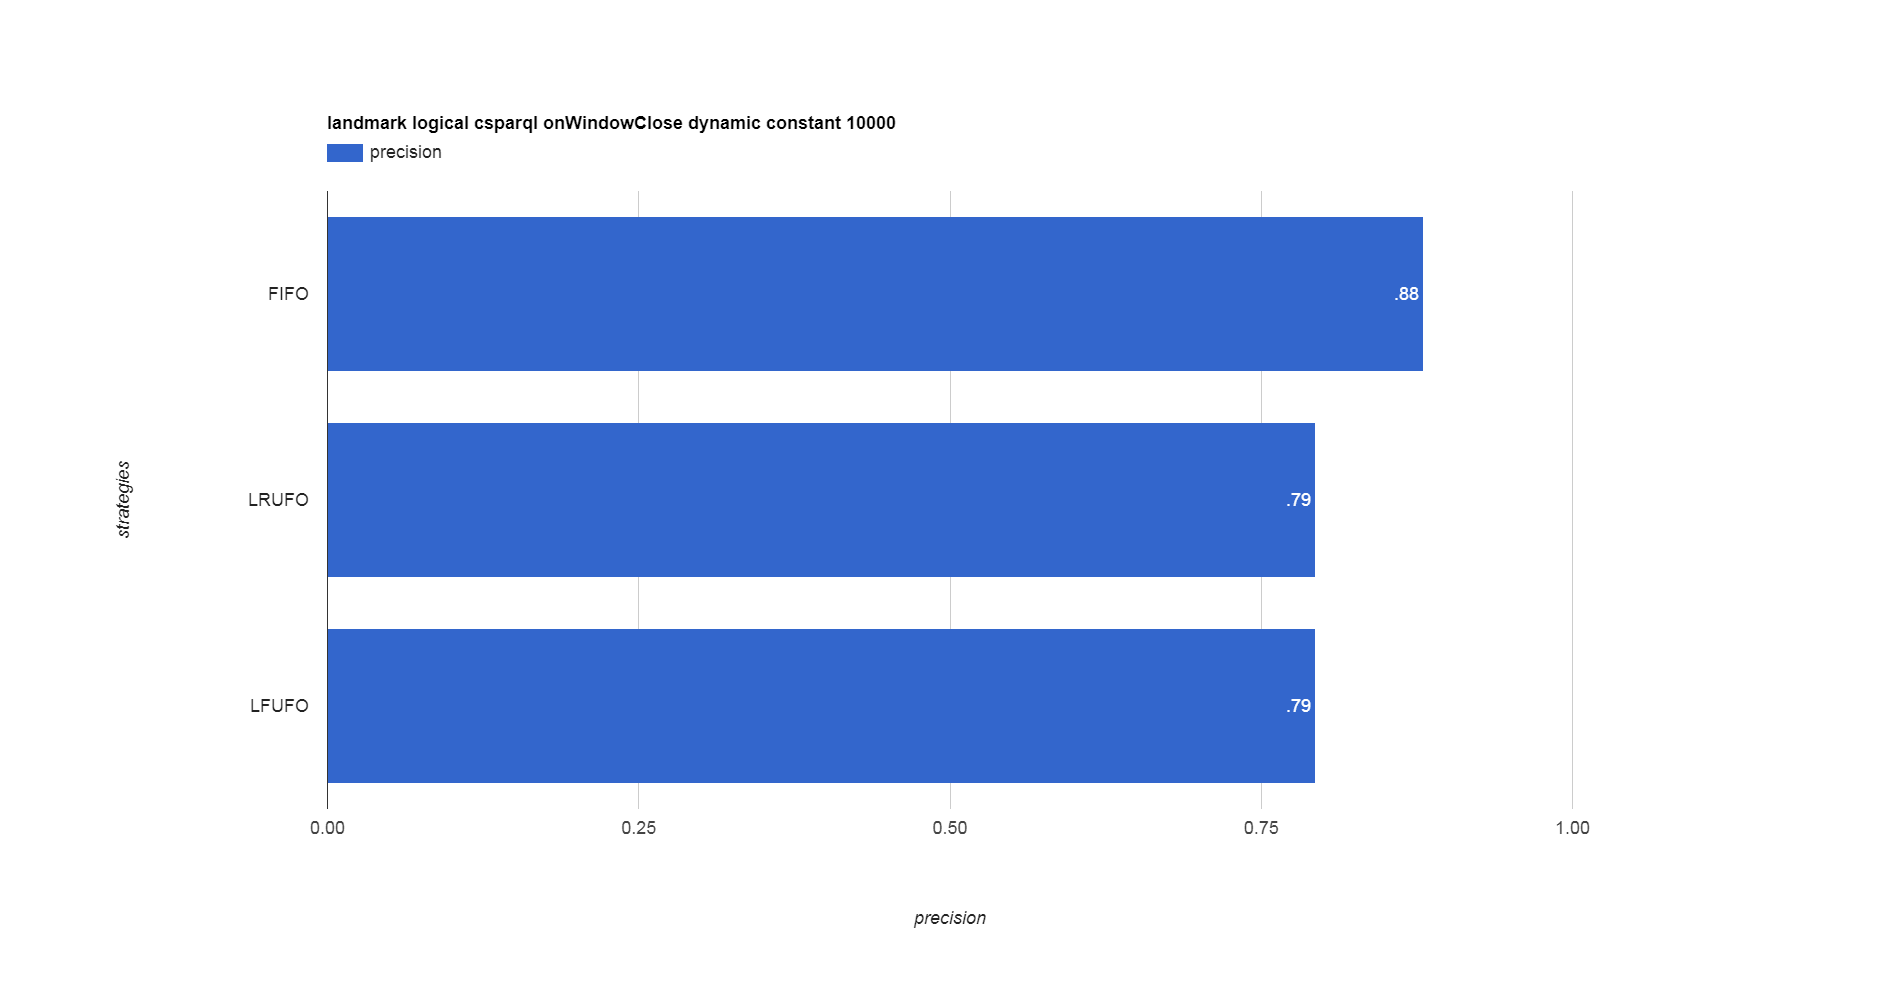
\includegraphics[width=\textwidth]{img/app3-qp-normal-p.png}
    \caption{Query Participation Normal Data Expiration Precision}
\end{figure}
\begin{figure}[!htbp]
    \centering
    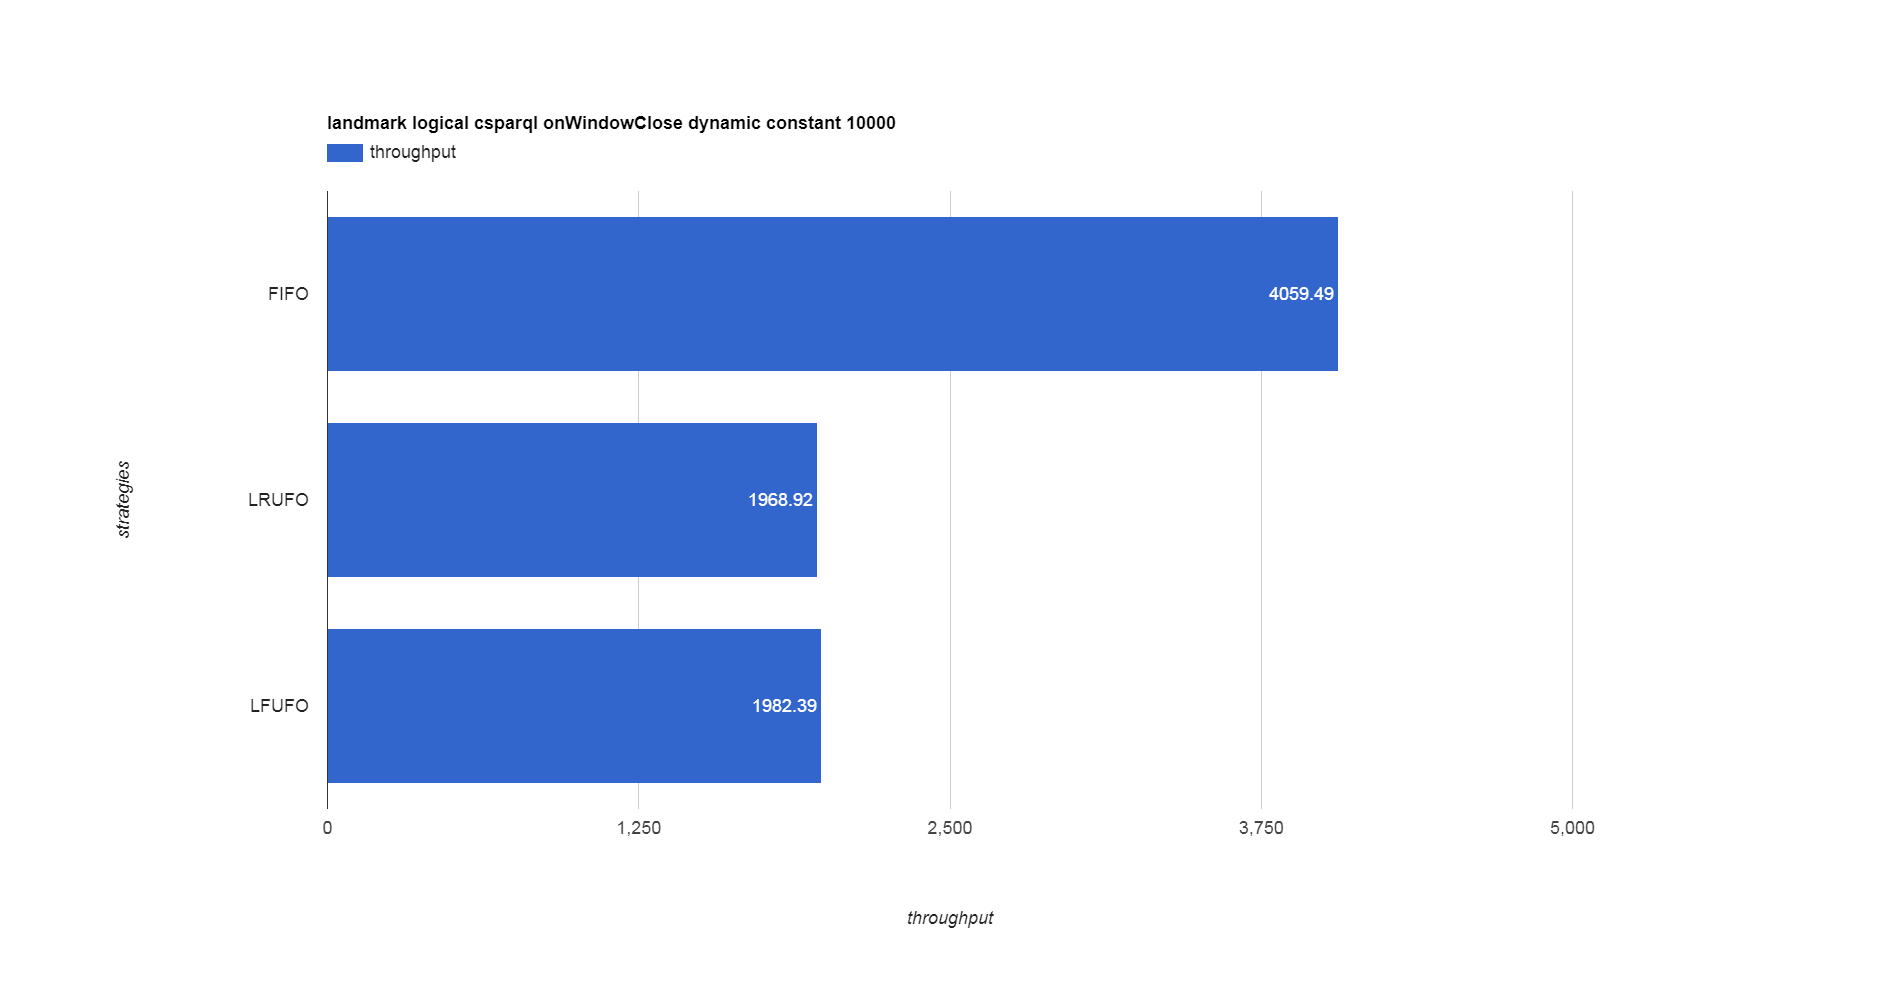
\includegraphics[width=\textwidth]{img/app3-qp-normal-t.png}
    \caption{Query Participation Normal Data Expiration Throughput}
\end{figure}
\begin{figure}[!htbp]
    \centering
    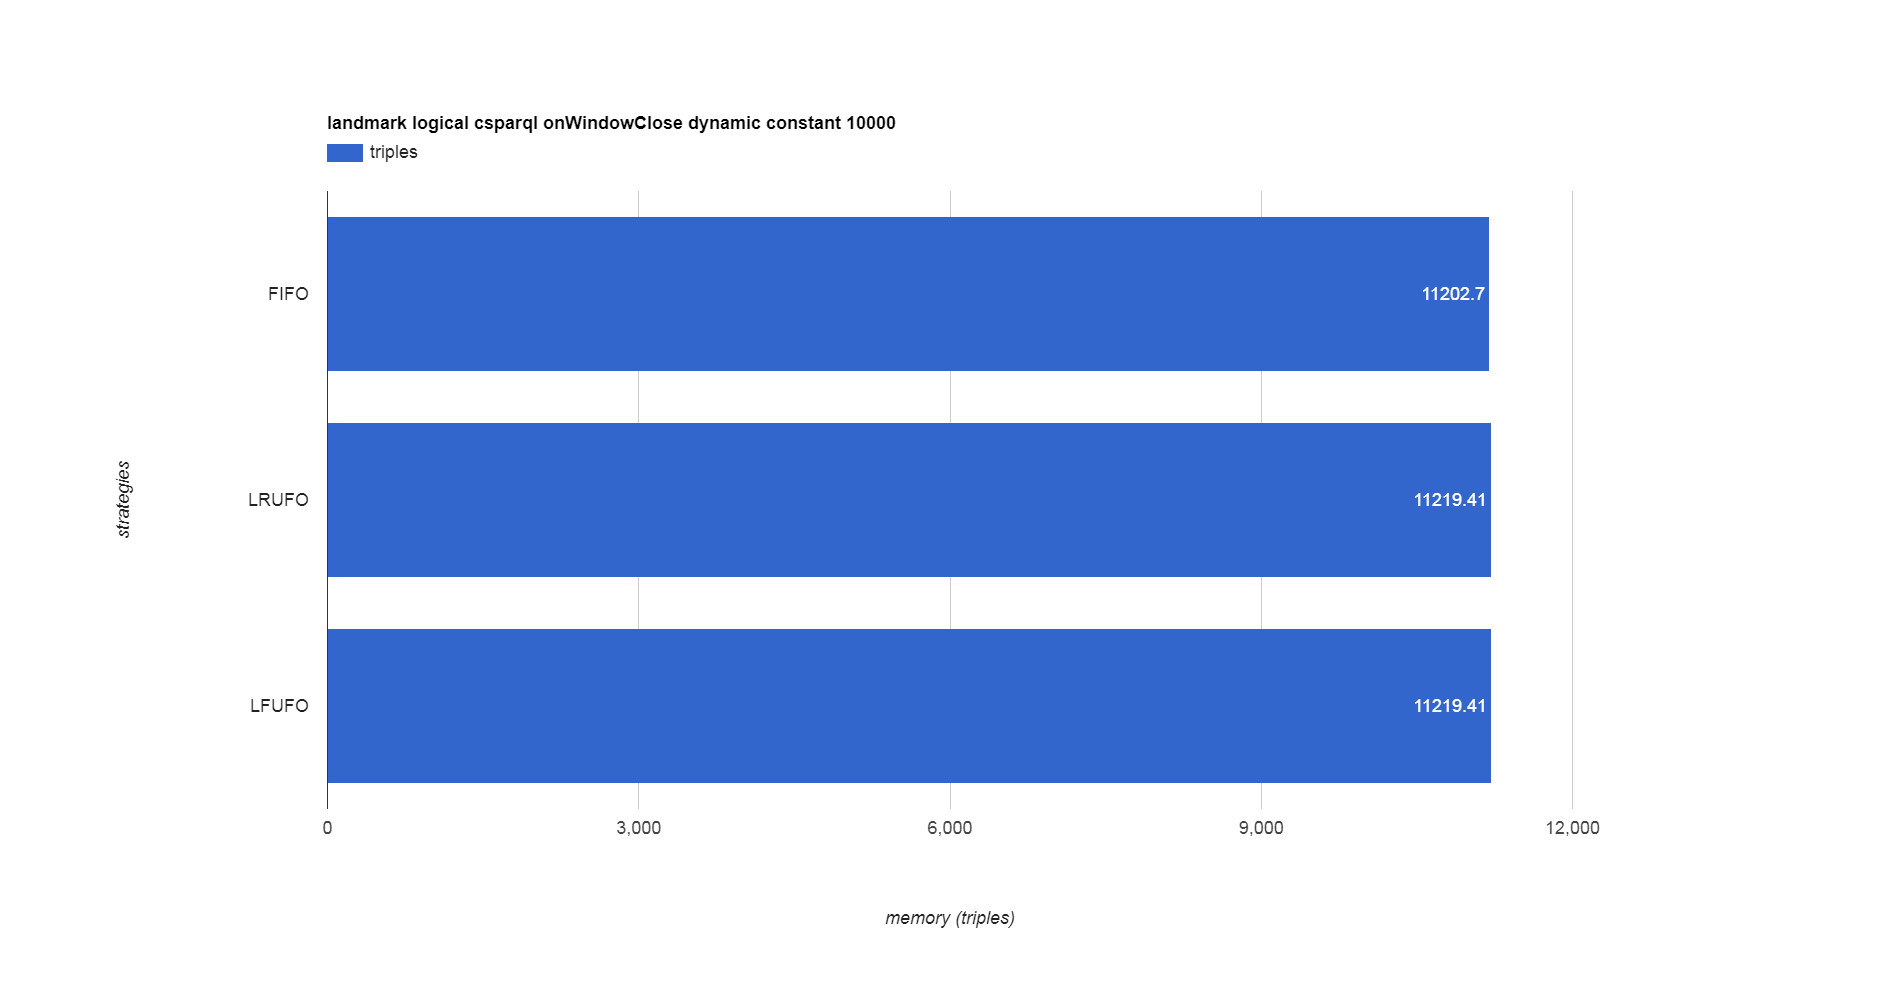
\includegraphics[width=\textwidth]{img/app3-qp-slow-m.png}
    \caption{Query Participation Slow Data Expiration Memory Consumption}
\end{figure}
\begin{figure}[!htbp]
    \centering
    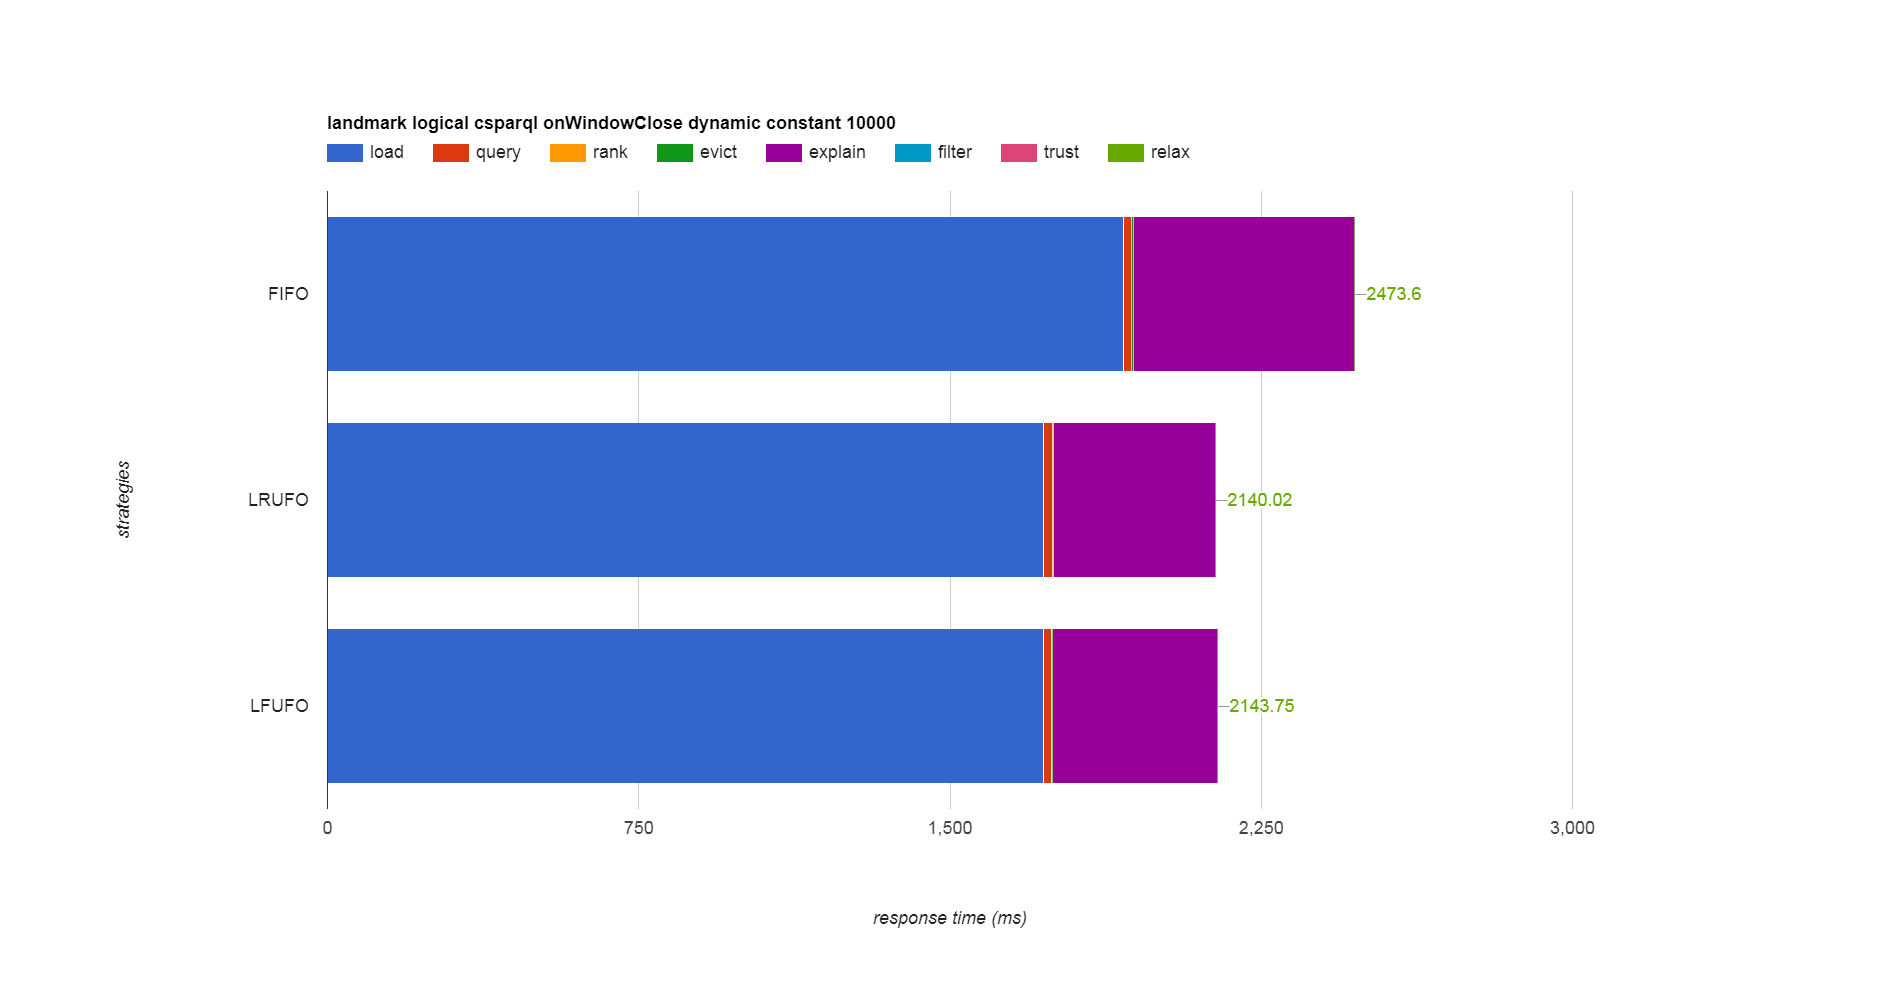
\includegraphics[width=\textwidth]{img/app3-qp-slow-r.png}
    \caption{Query Participation Slow Data Expiration Response Time}
\end{figure}
\begin{figure}[!htbp]
    \centering
    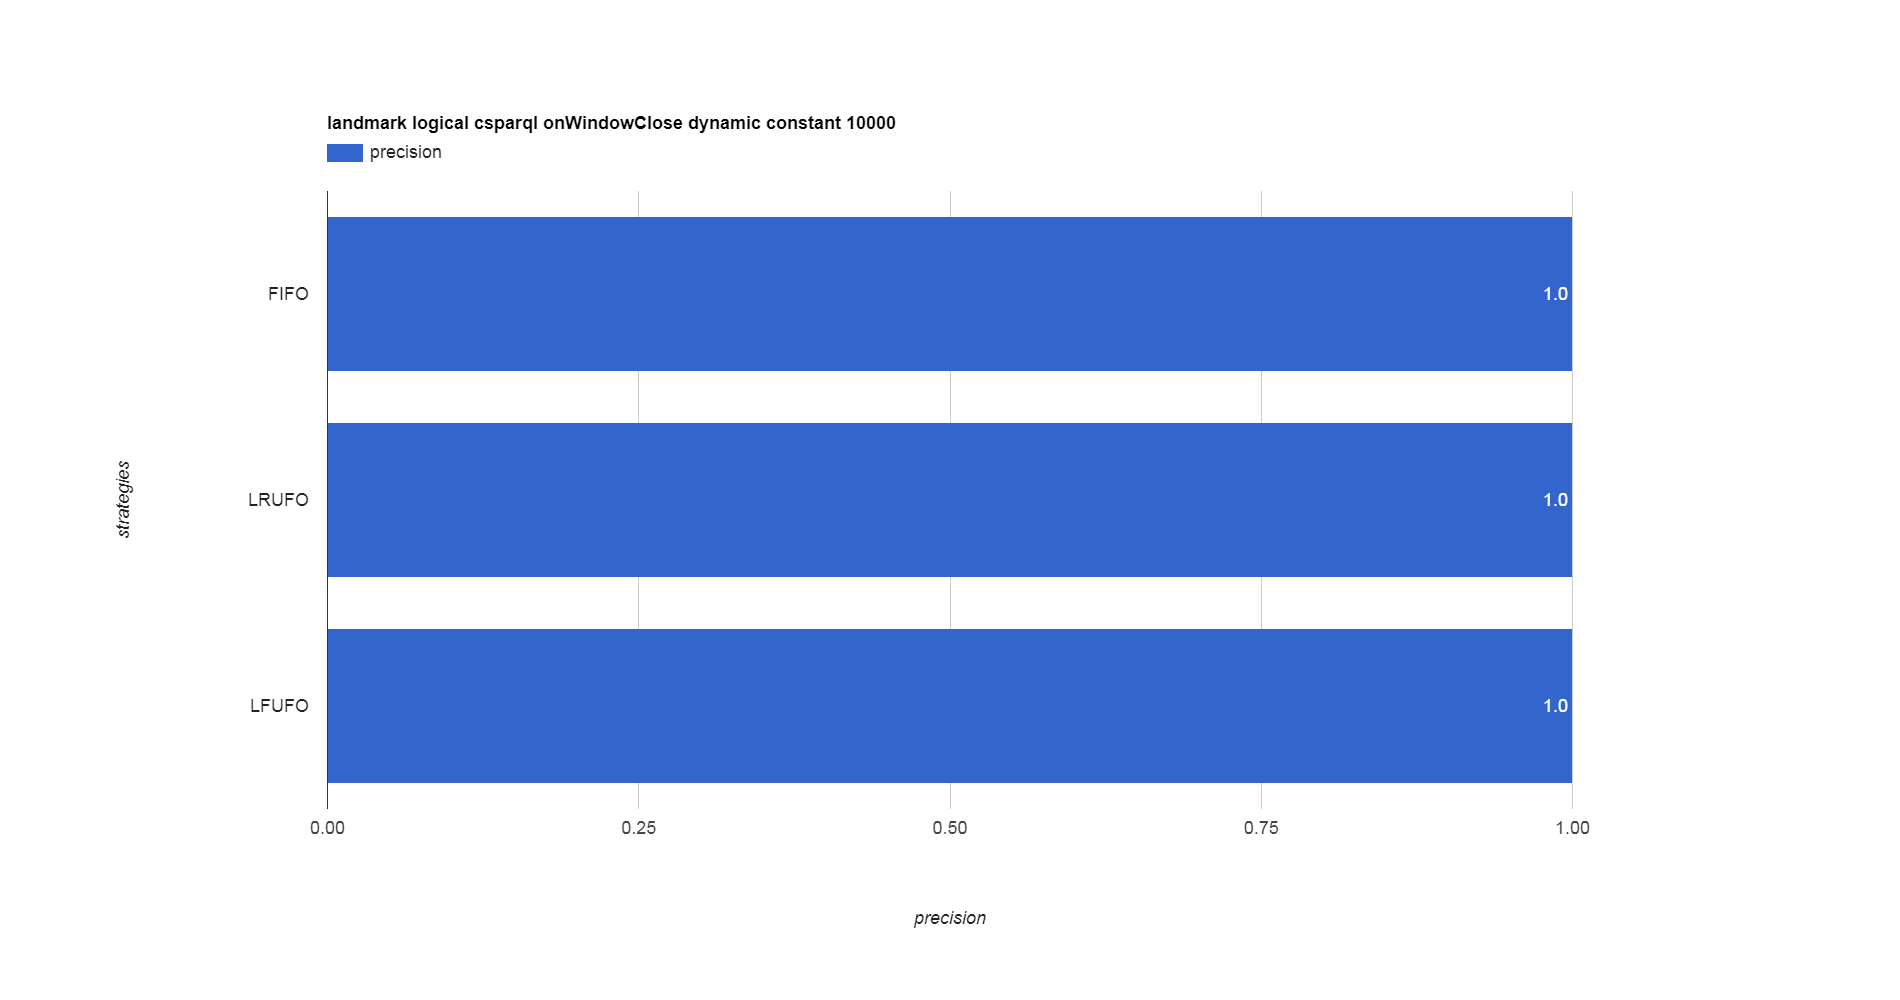
\includegraphics[width=\textwidth]{img/app3-qp-slow-p.png}
    \caption{Query Participation Slow Data Expiration Precision}
\end{figure}
\begin{figure}[!htbp]
    \centering
    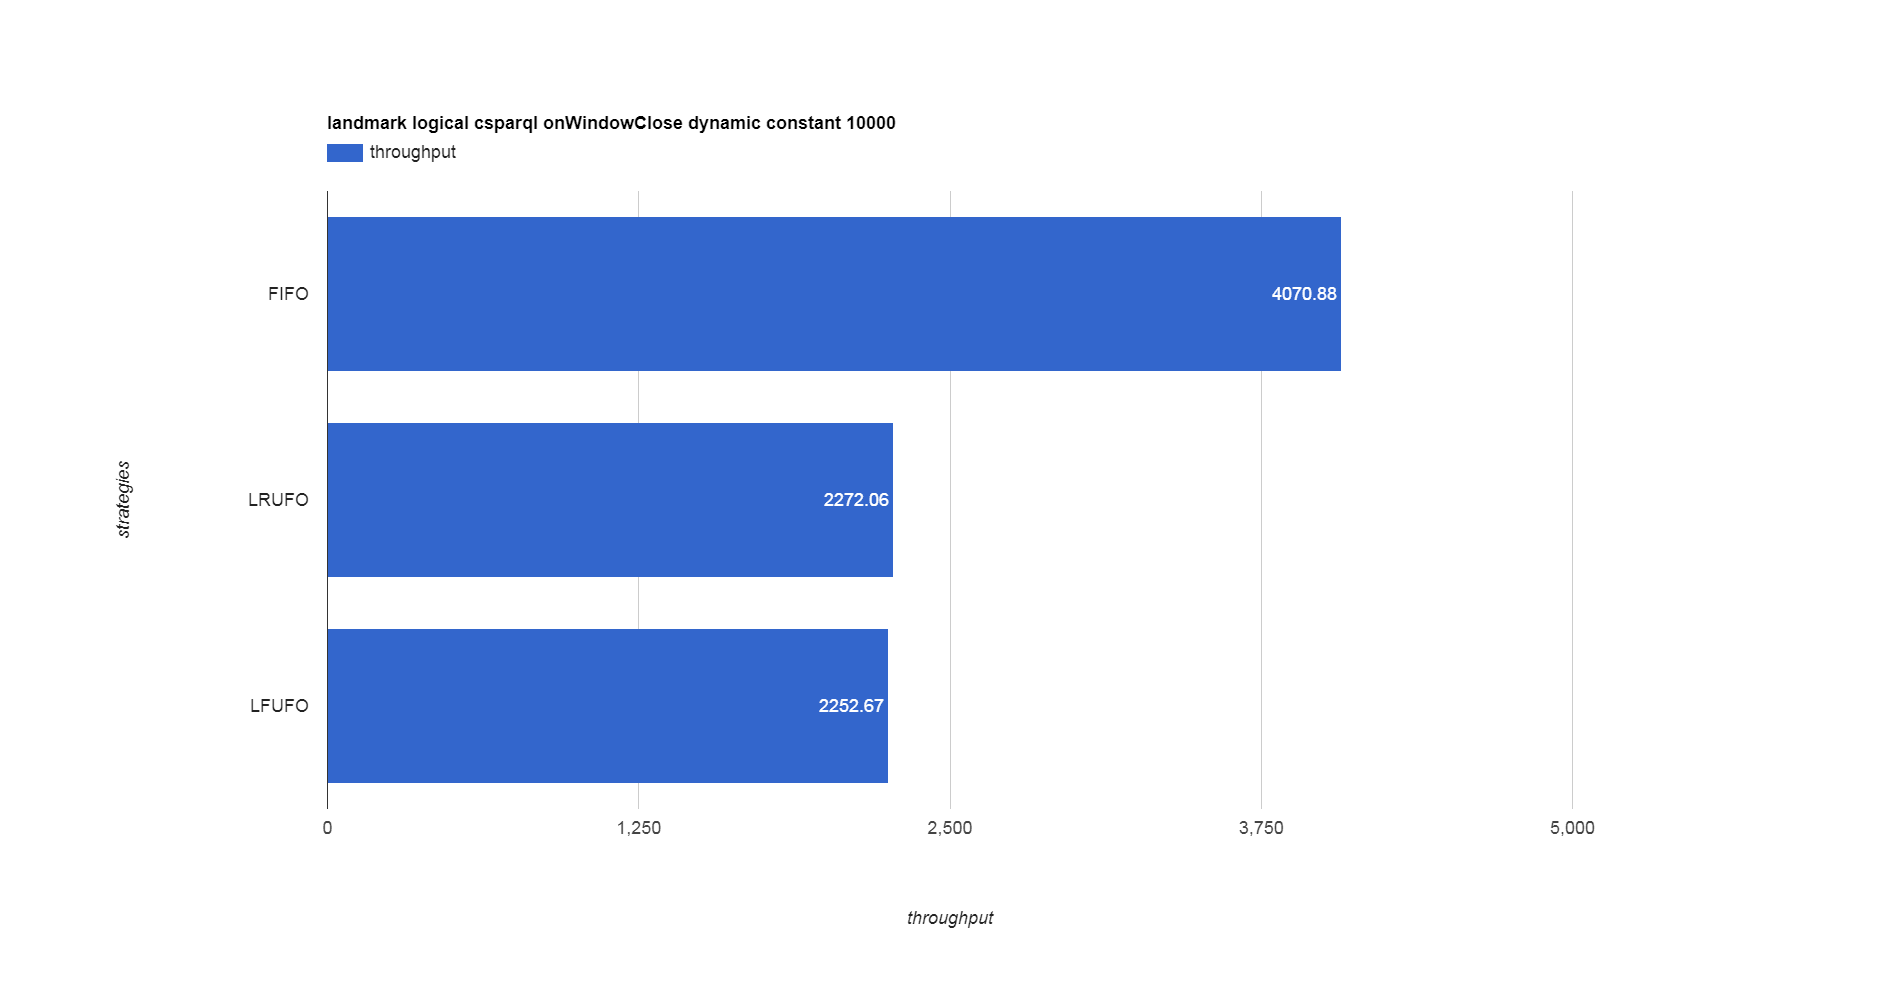
\includegraphics[width=\textwidth]{img/app3-qp-slow-t.png}
    \caption{Query Participation Slow Data Expiration Throughput}
\end{figure}
\begin{figure}[!htbp]
    \centering
    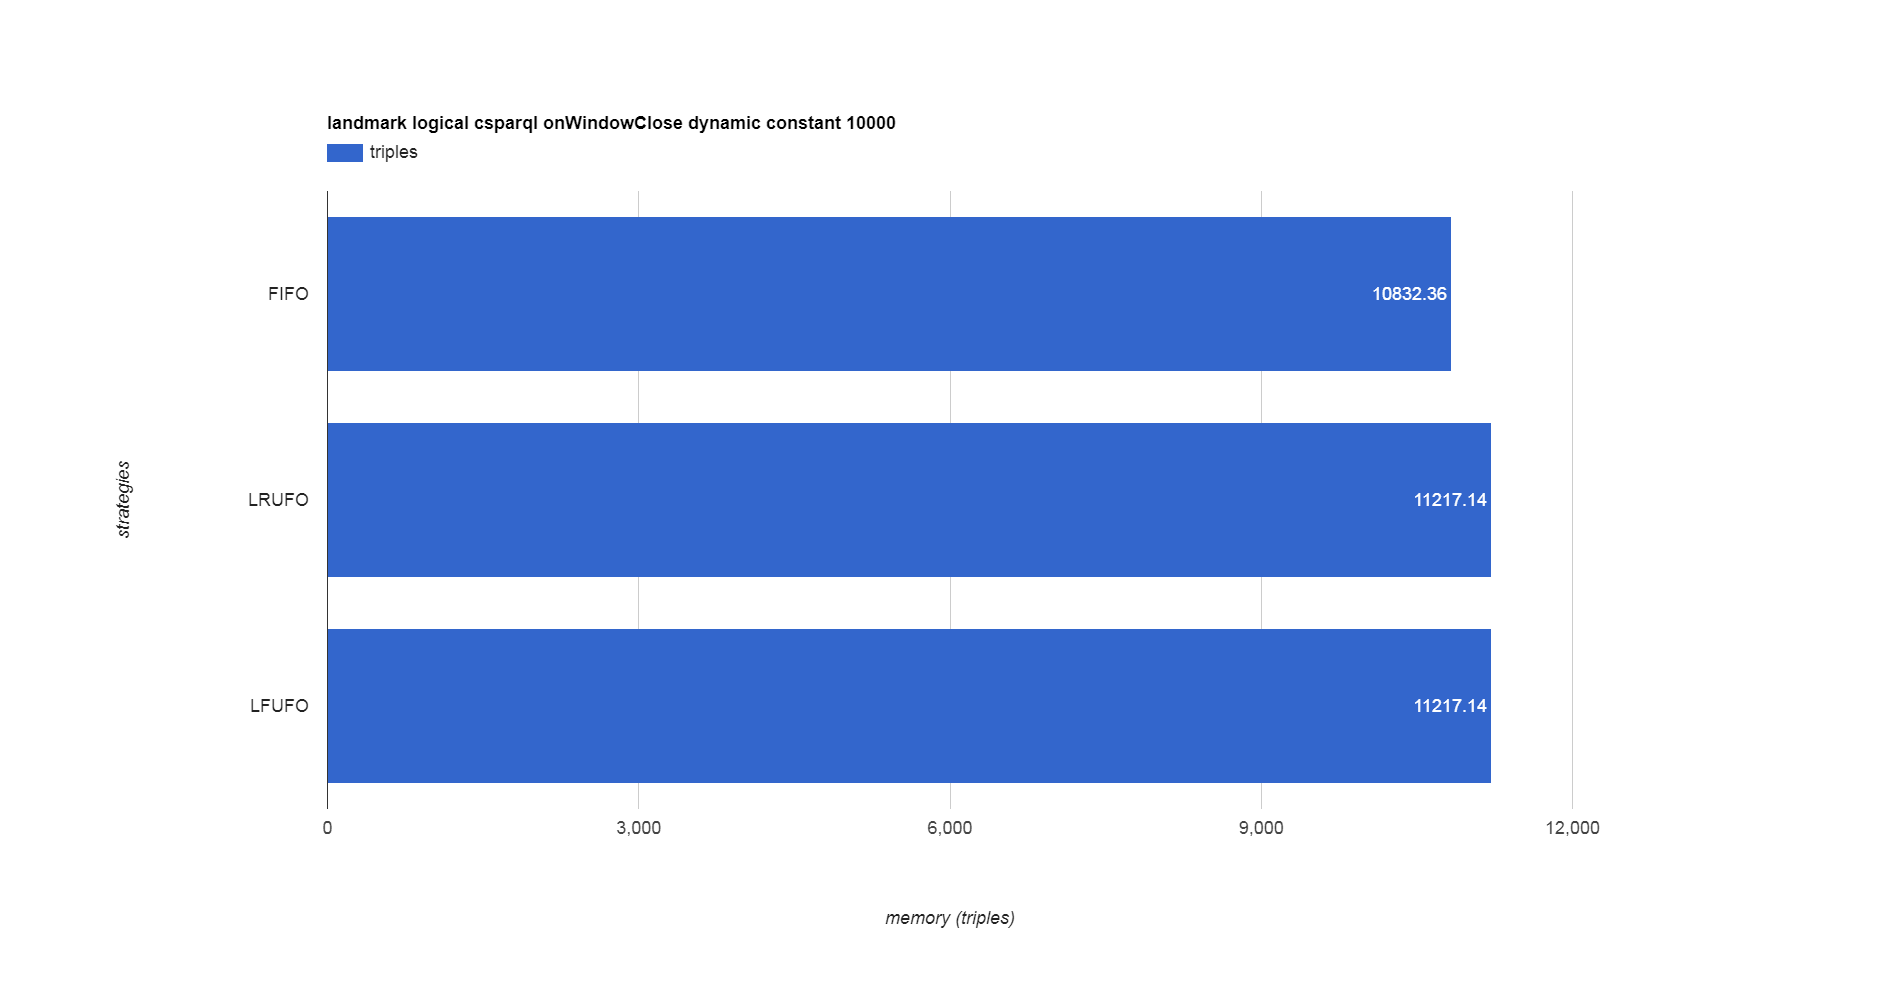
\includegraphics[width=\textwidth]{img/app3-qp-no-m.png}
    \caption{Query Participation No Data Expiration Memory Consumption}
\end{figure}
\begin{figure}[!htbp]
    \centering
    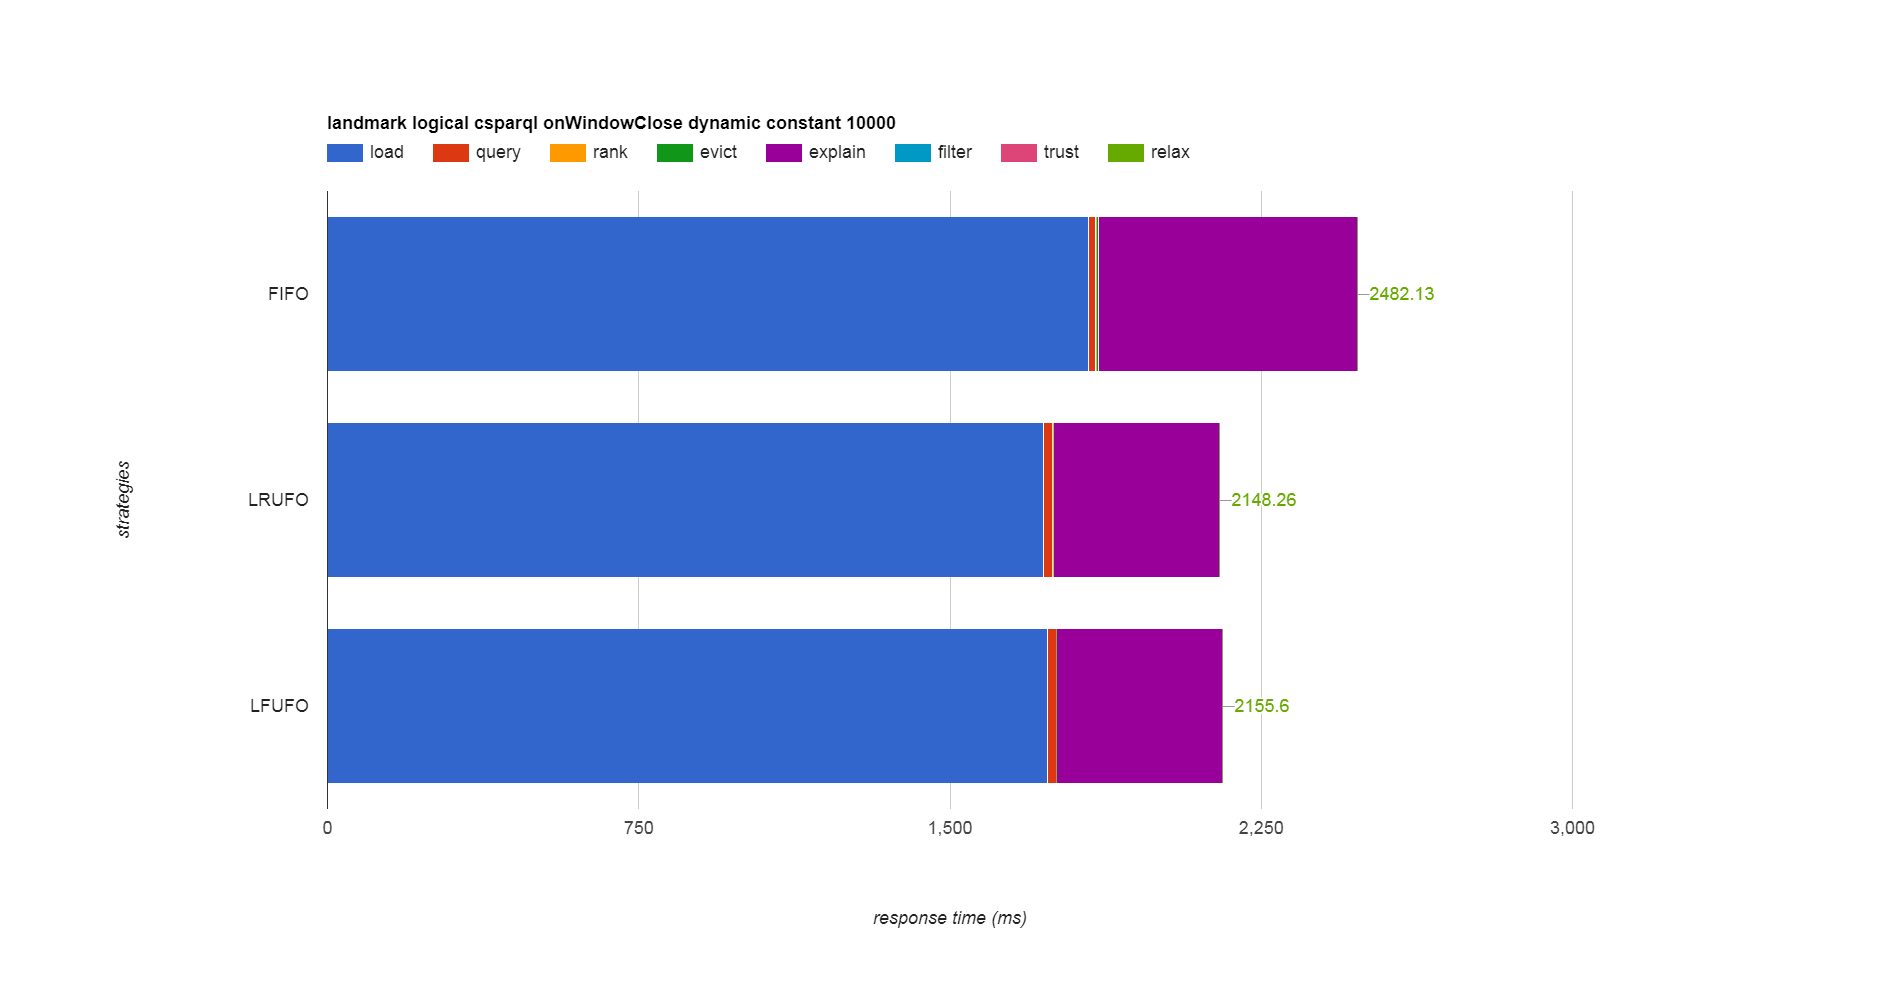
\includegraphics[width=\textwidth]{img/app3-qp-no-r.png}
    \caption{Query Participation No Data Expiration Response Time}
\end{figure}
\begin{figure}[!htbp]
    \centering
    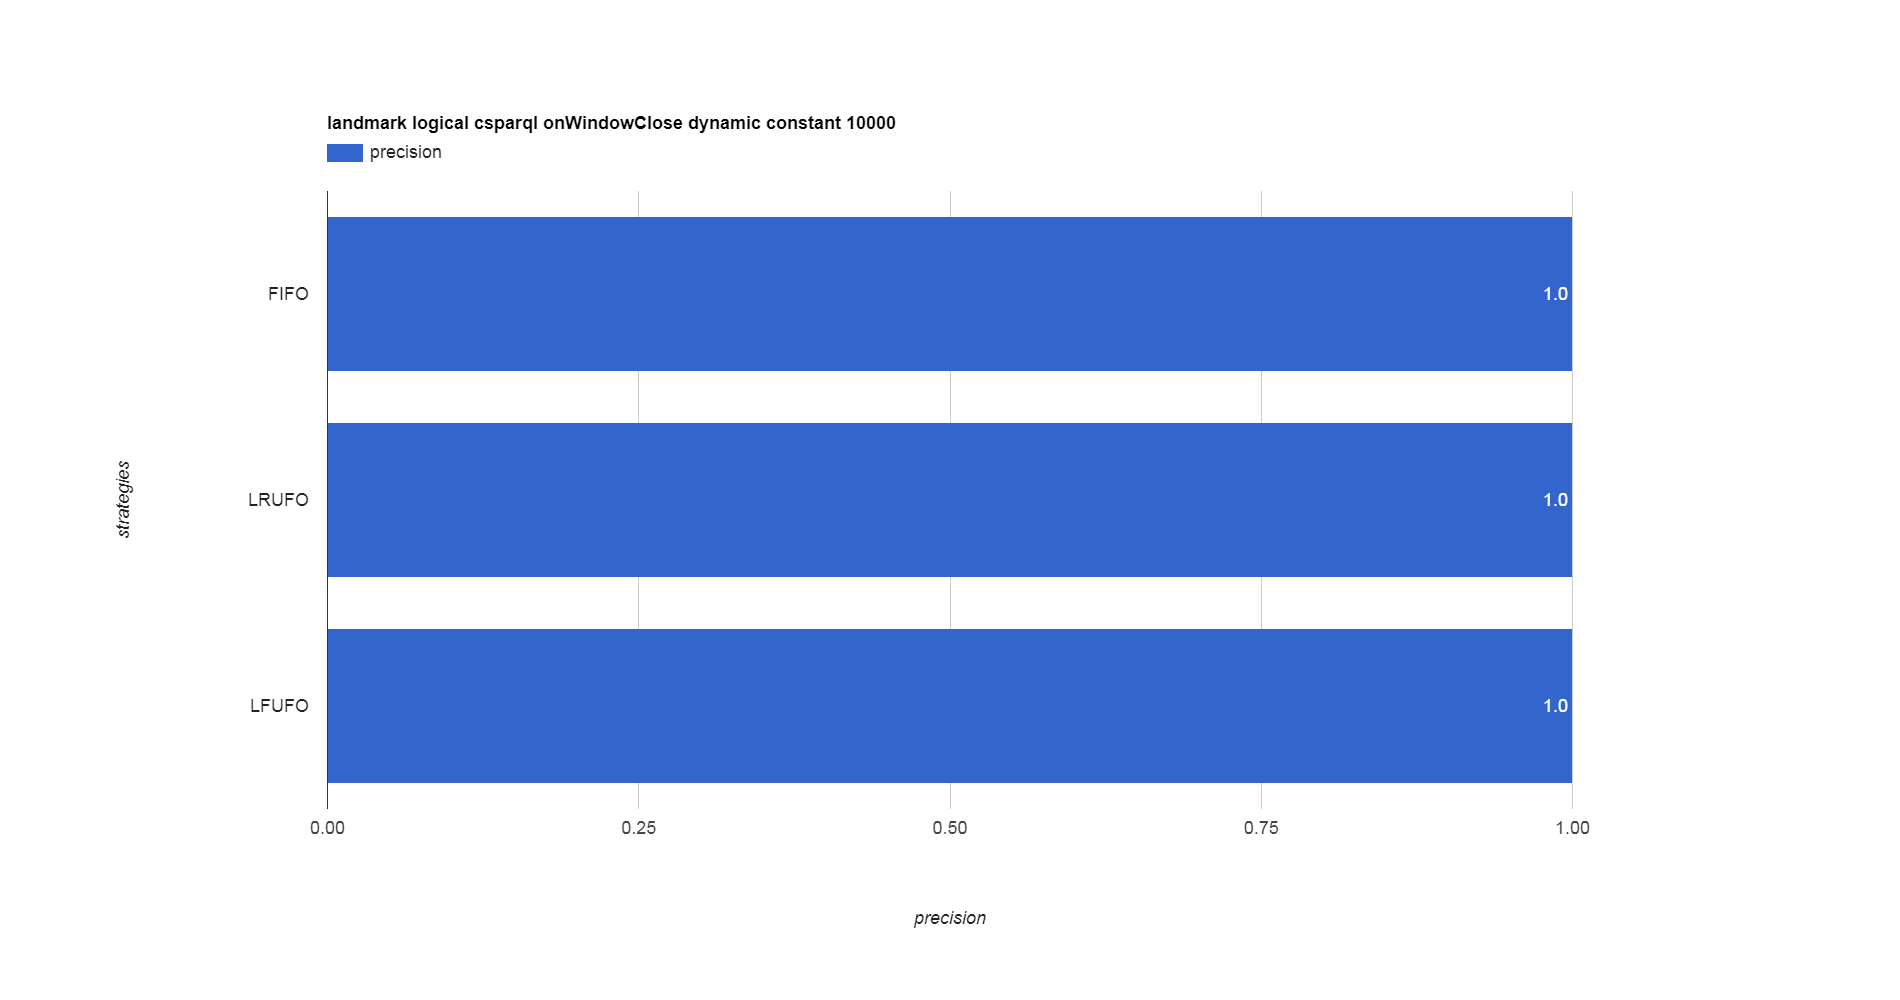
\includegraphics[width=\textwidth]{img/app3-qp-no-p.png}
    \caption{Query Participation No Data Expiration Precision}
\end{figure}
\begin{figure}[!htbp]
    \centering
    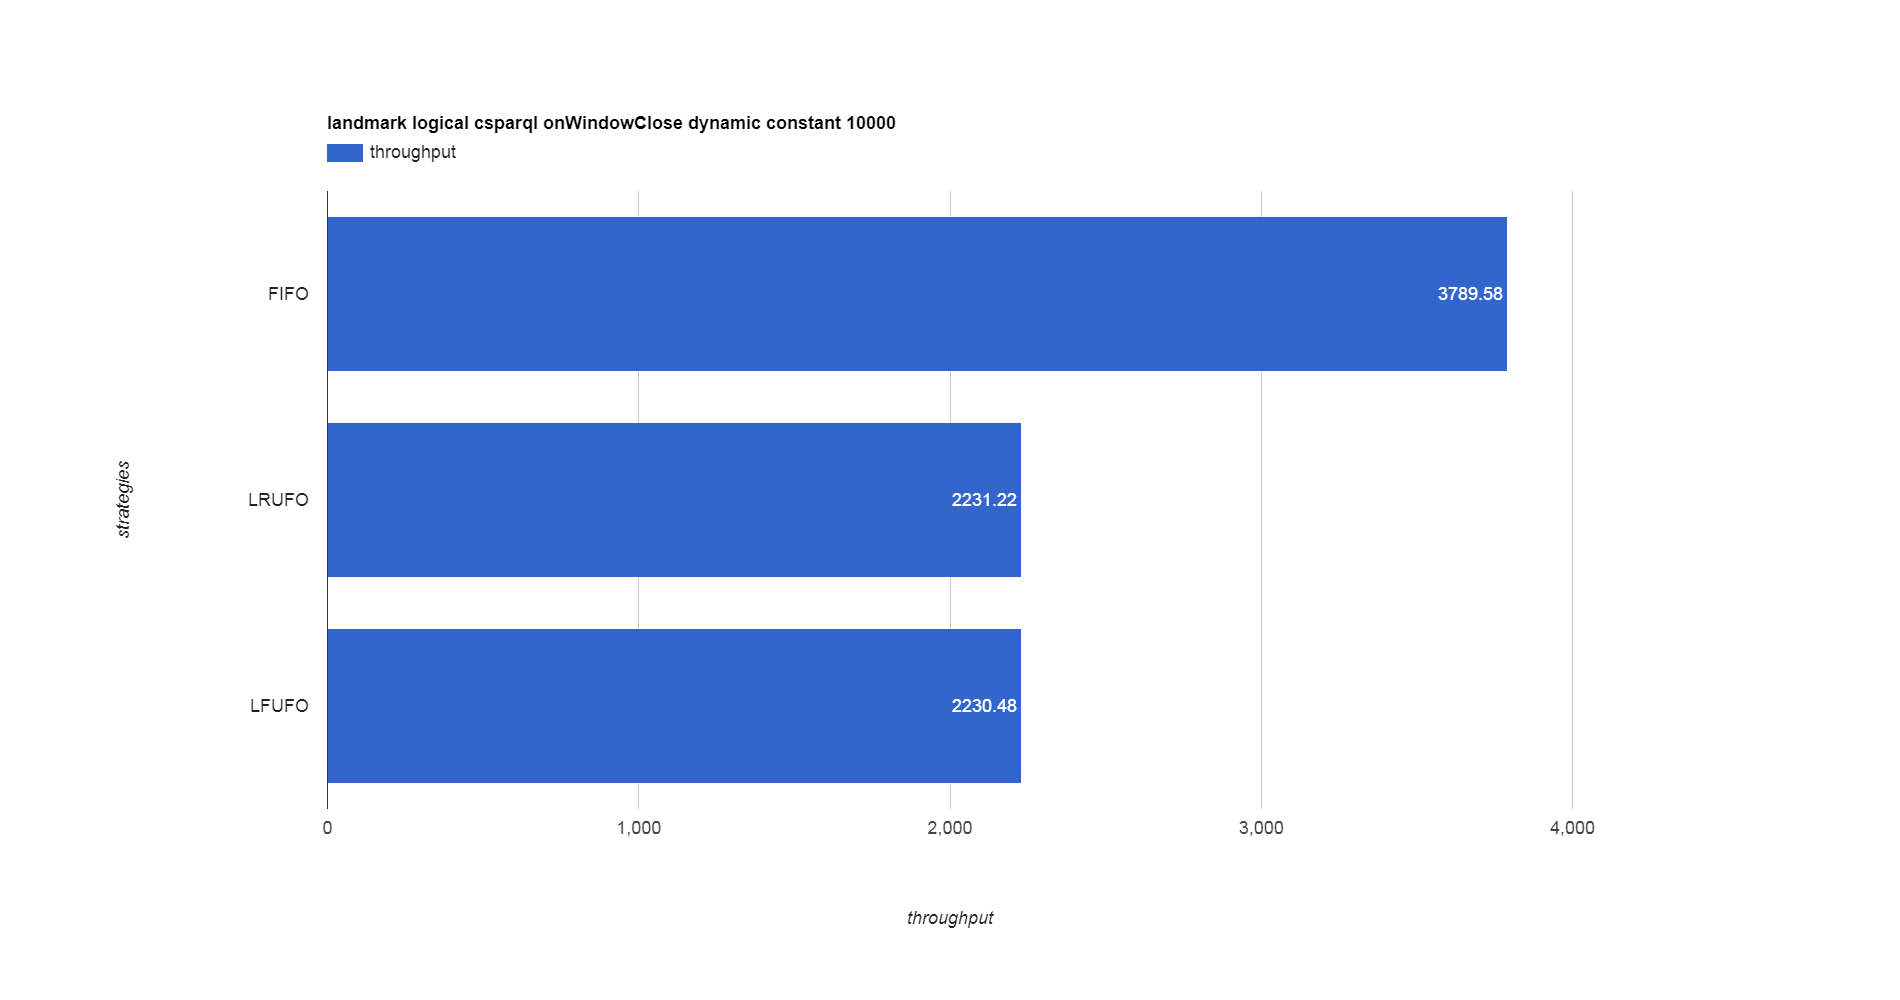
\includegraphics[width=\textwidth]{img/app3-qp-no-t.png}
    \caption{Query Participation No Data Expiration Throughput}
\end{figure}